\documentclass[oneside,numbers,spanish,a4paper]{ezthesis}
%\documentclass[oneside,authoryear,draft,spanish]{ezthesis}
%\documentclass[oneside,authoryear,draftmarks,spanish]{ezthesis}
%% # Opciones disponibles para el documento #
%%
%% Las opciones con un (*) son las opciones predeterminadas.
%%
%% Modo de compilar:
%%   draft            - borrador con marcas de fecha y sin im'agenes
%%   draftmarks       - borrador con marcas de fecha y con im'agenes
%%   final (*)        - version final de la tesis
%%
%% Tama'no de papel:
%%   letterpaper (*)  - tama'no carta (Am'erica)
%%   a4paper          - tama'no A4    (Europa)
%%
%% Formato de impresi'on:
%%   oneside          - hojas impresas por un solo lado
%%   twoside (*)      - hijas impresas por ambos lados
%%
%% Tama'no de letra:
%%   10pt, 11pt, o 12pt (*)
%%
%% Espaciado entre renglones:
%%   singlespace      - espacio sencillo
%%   onehalfspace (*) - espacio de 1.5
%%   doublespace      - a doble espacio
%%
%% Formato de las referencias bibliogr'aficas:
%%   numbers          - numeradas, p.e. [1]
%%   authoryear (*)   - por autor y a'no, p.e. (Newton, 1997)
%%
%% Opciones adicionales:
%%   spanish         - tesis escrita en espa'nol
%%
%% Desactivar opciones especiales:
%%   nobibtoc   - no incluir la bibiolgraf'ia en el 'Indice general
%%   nofancyhdr - no incluir "fancyhdr" para producir los encabezados
%%   nocolors   - no incluir "xcolor" para producir ligas con colores
%%   nographicx - no incluir "graphicx" para insertar gr'aficos
%%   nonatbib   - no incluir "natbib" para administrar la bibliograf'ia

%% Paquetes adicionales requeridos se pueden agregar tambi'en aqu'i.
%% Por ejemplo:
\usepackage{etex}
%\usepackage[caption=false]{subfig}
\usepackage{multirow}
\usepackage[activeacute,spanish]{babel}
\usepackage[utf8]{inputenc}
\usepackage{amsmath}
\usepackage{mathtools}
\usepackage{amsmath,amssymb,amsfonts,latexsym,cancel}
\usepackage{rawfonts}
\usepackage{pictexwd}
\usepackage{float}
\usepackage{mdwlist}
\usepackage{booktabs}
\usepackage{graphicx}
\usepackage{subcaption}
\numberwithin{equation}{section}
%paquete para diagramas
\usepackage[all]{xy}
\usepackage{mathrsfs}
%\usepackage{tikz}
%\usetikzlibrary{3d}
%\usepackage{tikz-3dplot}
\usepackage[thinlines]{easytable}
\usepackage[htt]{hyphenat}
%Configuracion codigo c++
\usepackage{listings}
\usepackage[T1]{fontenc}
\usepackage{times}
\usepackage{color}
\usepackage{units}
\usepackage{rotating}
\usepackage{pdfpages}
\definecolor{lightblue}{rgb}{0, 0.7, .7}
\definecolor{gray97}{gray}{.97}
\definecolor{gray75}{gray}{.75}
\definecolor{gray45}{gray}{.45}
\lstset{ frame=Ltb,
framerule=0pt,
aboveskip=0.5cm,
framextopmargin=3pt,
framexbottommargin=3pt,
framexleftmargin=0.4cm,
framesep=0pt,
rulesep=.4pt,
backgroundcolor=\color{gray97},
rulesepcolor=\color{black},
%
stringstyle=\ttfamily,
showstringspaces = false,
basicstyle=\tiny\ttfamily,
commentstyle=\color{gray45},
keywordstyle=\bfseries,
%
numbers=left,
numbersep=15pt,
numberstyle=\tiny,
numberfirstline = false,
breaklines=true,
}
% minimizar fragmentado de listados
\lstnewenvironment{listing}[1][]
{\lstset{#1}\pagebreak[0]}{\pagebreak[0]}

\lstdefinestyle{consola}
{basicstyle=\scriptsize\bf\ttfamily,
backgroundcolor=\color{gray75},
}

\lstdefinestyle{C}
{language=C,
}

\lstdefinestyle{customc}{
  belowcaptionskip=1\baselineskip,
  breaklines=true,
  frame=L,
  xleftmargin=\parindent,
  language=C,
  showstringspaces=false,
  basicstyle=\footnotesize\ttfamily,
  keywordstyle=\bfseries\color{green!40!black},
  commentstyle=\itshape\color{purple!40!black},
  identifierstyle=\color{blue},
  stringstyle=\color{orange},
}

\lstdefinestyle{customasm}{
  belowcaptionskip=1\baselineskip,
  frame=L,
  xleftmargin=\parindent,
  language=Matlab,
  basicstyle=\footnotesize\ttfamily,
  commentstyle=\itshape\color{purple!40!black},
  breaklines=true,
  breakatwhitespace=true,
  linewidth=1.1\linewidth
}

\lstset{escapechar=@,style=customasm,basicstyle=\small}
%
%\lstset{breaklines=true, language=Matlab}


%%##################################################################################################################################
%% # Datos del documento #
%% Nota que los acentos se deben escribir: \'a, \'e, \'i, etc.
%% La letra n con tilde es: \~n.

\author{Sebastián Orlando Cueto del Fierro}

\title{``ESTUDIO EXPERIMENTAL DEL COMPORTAMIENTO DE FATIGA PARA EL MATERIAL ABS IMPRESO EN 3D''}
\degree{Ingeniería Mecánica Industrial }
\supervisor{Ph.D. Alejandro Pacheco Sanjuan}
\correferent{Dra. Sheila Lascano Farak}
\institution{UNIVERSIDAD TÉCNICA FEDERICO SANTA MARÍA}
\faculty{Escuela de Ingeniería y Ciencias}
\department{DEPARTAMENTO DE INGENIERÍA MECÁNICA}
\city{VALPARAÍSO}
\country{CHILE}

%% # M'argenes del documento #
%% 
%% Quitar el comentario en la siguiente linea para austar los m'argenes del
%% documento. Leer la documentaci'on de "geometry" para m'as informaci'on.

\geometry{top=35mm,bottom=35mm,inner=30mm,outer=30mm}

%\DeclareUnicodeCharacter{202F}{FIX ME!!!!}

%% El siguiente comando agrega ligas activas en el documento para las
%% referencias cruzadas y citas bibliogr'aficas. Tiene que ser *la 'ultima*
%% instrucci'on antes de \begin{document}.
\hyperlinking

\begin{document}

\renewcommand{\listtablename}{Índice de tablas}
\renewcommand{\tablename}{Tabla} 
\renewcommand*{\appendixname}{Anexo}

\sloppy 


%% En esta secci'on se describe la estructura del documento de la tesis.
%% Consulta los reglamentos de tu universidad para determinar el orden
%% y la cantidad de secciones que debes de incluir.

%% # Portada de la tesis #
%\include{Portada/anteportada}
%%%Pagina en blanco sin numeracion
\newpage
$\ $\\
\thispagestyle{empty}
\include{Preliminares/portada}
%%%Pagina en blanco sin numeracion
\newpage
$\ $\\
\thispagestyle{empty}
%\include{Preliminares/contraportada}

%% # Prefacios #
%% Por cada prefacio (p.e. agradecimientos, resumen, etc.) crear
%% un nuevo archivo e incluirlo aqu'i.
%% Para m'as detalles y un ejemplo mirar el archivo "gracias.tex".
\thispagestyle{empty}
\vspace*{\fill}
\begin{quote}
	\raggedleft
	\emph{The more we learn about the world, and the deeper our learning, the more conscious, specific, and articulate will be our knowledge of what we do not know, our knowledge of our ignorance. For this, indeed, is the main source of our ignorance — the fact that our knowledge can be only finite, while our ignorance must necessarily be infinite}
	
	\bigskip
	\emph{Karl Popper}
\end{quote}
\vspace*{\fill}



%%% Las secciones del "prefacio" inician con el comando \prefacesection{T'itulo}
%% Este tipo de secciones *no* van numeradas, pero s'i aparecen en el 'indice.
%%
%% Si quieres agregar una secci'on que no vaya n'umerada y que *tampoco*
%% aparesca en el 'indice, usa entonces el comando \chapter*{T'itulo}
%%
%% Recuerda que aqu'i ya puedes escribir acentos como: 'a, 'e, 'i, etc.
%% La letra n con tilde es: 'n.

\prefacesection{Agradecimientos}
Es difícil escribir y sintetizar en un par de párrafos los agradecimientos a un grupo de personas que han aparecido a lo largo de estos 8 años. Mis agradecimientos van principalmente hacia aquellas personas que me han marcado profundamente en este proceso, pero también hacia aquellas personas que de alguna o otra forma incidieron en mi paso por la universidad, incluso a aquellos que no conocí ni saludé. Son estos dos conjuntos de personas quienes agradezco por ser parte de este devenir, quienes en algún punto influyeron en mis tiempos, mis decisiones y todo aquello sobre lo que no tuve control, pero que finalmente, se acoplaron para poder dar cierre a este ciclo de mi vida.

Quiero agradecer a mi familia, a mi mamá y papá por apoyarme durante toda esta etapa, por permitirme el privilegio de dedicarme exclusivamente a los estudios y a otras cosas, inclusive. Por brindarme todas las herramientas necesarias, desde que nací hasta hoy, entregándome su tiempo, disposición y amor sin esperar retribución alguna, por retarme y alentarme cuando fuese necesario, pero por sobretodo por creer en mí y en mis capacidades. A mi abuela Rosa y mi abuelo Hernán, quienes llegaron a ser unos segundos padres al consintirme, formarme e impregnarme de su amor por los libros, la música, los relatos y su cariño.

Por otro lado, también agradezco a mis amigas Susi, Camila y Catalina, a mis amigos Patricio, Marcelo, Pablo Campos, Pablo Kohler, Cristián, Sebastián y Pablo Cárdenas, quienes conozco desde mis primeros años en la universidad o antes, que me apoyaron en los momentos difíciles y me felicitaron en los momentos alegres. Les agradezco su capacidad de discusión, de poder opinar libremente y la idea de siempre buscar construirnos como mejores personas, por su infaltable cariño y afecto que hizo más ameno mi paso por la universidad, en especial a los tres últimos quienes me ayudaron a desarrollar esta tesis con sus conocimientos y el abrirse a escucharme. Por otro lado, quiero agradecer a Laura, quien fue mi amiga y compañera, por su inconmensurable amor, dedicación y paciencia, por su capacidad de creer en mí, aún en los momentos más oscuros. No fueron sino las risas, la compañía y su sabiduría lo que me permitieron llegar hasta donde estoy.

A mis compañeros de banda, con quienes durante 8 años ensayamos, compartimos y nos enseñamos alrededor de la música. La excusa de juntarse a tocar instrumentos de forma coordinada desencadenó en una amistad y un espacio de aprendizaje profundo que sobrepasa las dimensiones de la banda misma. Sin duda, cada ensayo y cada creación fueron un escape de la universidad, permitiéndonos dialogar y expresarnos a través de nuestra música, pero también al abrirnos y exponer nuestros sentimientos en la conversación.

Al profesor Alejandro Pacheco, con quien tuve la suerte de desarrollar esta tesis, contar con su apoyo e infinita paciencia. La dedicación que tuvo al destinar de su tiempo para enseñarme, responder mis dudas y corregirme cada vez que me equivocaba fueron una constante luz en este largo proceso.  Sin duda su empuje a estudiar, comprender y aplicar lo aprendido me dejo una marca importante en mi formación que espero lograr plasmar en mi futuro como ingeniero. 

Finalmente, me gustaría agradecer a don Vicente Álvarez, apoyo académico del laboratorio de tecnología mecánica, quien siempre estuvo dispuesto a ayudarme, enseñarme y abrir la máquina un sin número de veces, sus palabras de ánimo y grata disposición fueron un gran apoyo y facilitó en gran medida el desarrollo de este trabajo.



%%Pagina en blanco sin numeracion
\newpage
$\ $\\
\thispagestyle{empty}
%%% Las secciones del "prefacio" inician con el comando \prefacesection{T'itulo}
%% Este tipo de secciones *no* van numeradas, pero s'i aparecen en el 'indice.
%%
%% Si quieres agregar una secci'on que no vaya n'umerada y que *tampoco*
%% aparesca en el 'indice, usa entonces el comando \chapter*{T'itulo}
%%
%% Recuerda que aqu'i ya puedes escribir acentos como: 'a, 'e, 'i, etc.
%% La letra n con tilde es: 'n.
\prefacesection{Abstract}

This work is developed around the flexural fatigue machine from mechanics technology laboratory, to move forward into its operativeness. The work methodology of this work is divided in 4 stages: get information about the machine, structural machine support design, machine modeling behaviour and contrast the previous information with results.

Nowadays, issues in the normal operavility by the machine and unavailable spares, made it unsuitable for operation. Its functioning is based on a unbalanced rotatory disc, by counterweights, to produce a specific stress.

The structural machine support was designed in wood and steel, using standard guide NCh 1198. It was simulated its static and modal behaviour, by means of FEM, to bear out the proposed design.

To characterize the machine behaviour, a dynamic model of the system was proposed. Through it, the loading arm movement and velocity are obtained. From this information, the force applied in the specimens is calculated for every configuration, achieving a relationship between $F_{max}$, $\omega_{max}$ and $\Delta m$ as a system variables.

The maximum force results, for a rotary disc velocity $\omega_{max}=1500$ rpm, are simulated using FEM to relate stress and strain state of the specimen with each configuration. Futhermore, using the relationship between each variables, it is founded the unbalance $\Delta m_y$ for yielding stress and $\Delta m_u$ for ultimate tensile strenght in the specimen. Lastly, fatigue life ($N_f$) is calculated for each configuration.

Thus, was possible to conclude that an update and maintenance was needed, as well as build the structural machine support to return the correct operation of the machine. On the other hand, there was discrepancies between the proposed model and the previus information. Hence, experimental validation are necessary as a later work.
%%%Pagina en blanco sin numeracion
\newpage
$\ $\\
\thispagestyle{empty}
%\prefacesection{Resumen}

Este trabajo se desarrolla entorno a la máquina de fatiga en flexión del laboratorio de tecnología mecánica, el cual tiene como objetivo avanzar hacia la operatividad de la misma. Para esto, la metodología se dividió en 4 etapas: levantamiento de información, diseño de una estructura soportante, modelar el comportamiento de la máquina y contrastar los resultados con la información existente.

Actualmente, la máquina no se encuentra operativa al presentar problemas en su funcionamiento y la disponibilidad de repuestos. Su funcionamiento se basa en aplicar una carga sobre la probeta mediante un disco desbalanceado a través de contrapesos, con una velocidad de rotación determinada para obtener un esfuerzo en específico.

La estructura soportante fue diseñada en base a madera y acero, utilizando como guía la norma NCh 1198. Se simuló mediante MEF su comportamiento estático y modal para corroborar el diseño propuesto.

Para caracterizar el comportamiento de la máquina, se propone un modelo dinámico del sistema. A través de este, se obtiene el movimiento y la velocidad del brazo de carga. A partir de esta información, se calcula la fuerza realizada sobre la probeta para cada configuración, logrando relacionar las variables del sistema $F_{max}$, $\omega_{max}$ y $\Delta m$. 

Los resultados de fuerza máxima se simularon utilizando MEF, para relacionar el estado de esfuerzos y deformación de la probeta con cada configuración de contrapesos, a una velocidad de rotación del disco $\omega_{max}=25$ rad/s. Además, utilizando las relaciones entre las variables, se encuentra el desbalanceo necesario para alcanzar la fluencia ($\Delta m_y$) y el esfuerzo último ($\Delta m_u$) de la probeta. Por último, se calcula la vida a fatiga ($N_f$) para cada configuración.

La información recopilada y los resultados obtenidos, se puede concluir que es necesaria una actualización y reparación de la máquina de fatiga, como también la construcción de la estructura soportante para lograr su operatividad. Por otro lado, existen discrepancias entre el modelo propuesto y la información existente, ante lo cual es necesario hacer un trabajo posterior de validación experimental sobre el comportamiento de la máquina.

%--------------------------------------------------------------------------------------------------------------

%El desarrollo de este trabajo se encuentra entorno a la máquina de fatiga en flexión del laboratorio de tecnología mecánica, el cual tiene como objetivo avanzar hacia la operatividad de la máquina. Para esto, la metodología se dividió en 4 etapas: levantamiento de información, diseño de una estructura soportante, modelar el comportamiento de la máquina y contrastar los resultados con la información existente.
%
%La máquina tiene problemas en su funcionamiento, mantenibilidad y disponibilidad de respuestos producto de su antigüedad. Su funcionamiento se basa en una tabla de cargas (anexo \ref{sec:anexob1}), que relaciona los contrapesos con los esfuerzos sobre probeta.

%El diseño de la estructura se realizó de acero y madera, utilizando como guía la norma NCh 1198. Además, a través de MEF se simuló el comportamiento estático y modal de la estructura. De esta manera, la dimensión final de cada componente se exponen en los planos del anexo \ref{sec:planos}.

%Para el modelamiento de la máquina, se utilizaron los datos obtenidos en el levantamiento de información y se resolvieron las ecuaciones de movimiento utilizando el método de energía. Así, se obtuvo el movimiento y la velocidad del centro de masa del brazo de carga. A través de esto, se calculó la fuerza realizada sobre la probeta para distintas configuraciones. La carga máxima posible, según el modelo, es de $1498.83$ [N], a una velocidad de rotación del disco $\omega_{max} =$ 25 [rad/s]. 

%Estos resultados de fuerza máxima se simularon usando MEF, utilizando como límite el esfuerzo último del material. Por lo tanto, se obtuvo una nueva relación entre las combinaciones de los contrapesos y los esfuerzos en la probeta, las cuales se muestran en la propuesta \ref{sec:anexob2}.  

%Con la información y los resultados obtenidos, se puede concluir que es necesaria una actualización y reparación de la máquina de fatiga, como también la construcción de la estructura para lograr que la máquina este operativa. Además existen discrepancias entre el modelo propuesto y la información existente, ante lo cual es necesario hacer un trabajo posterior que valide, refute o corrija el modelo y la tabla de cargas propuesta. 

%--------------------------------------------------------------------------------------------------------------

%El desarrollo de este trabajo se encuentra entorno a la máquina de fatiga en flexión del laboratorio de tecnología mecánica, en Valparaíso. Actualmente no se encuentra operativa, por lo tanto, el objetivo de este trabajo es avanzar en la dirección que permita volver a tener operativa la máquina. Para esto, la metodología de trabajo se dividió en 4 grandes etapas: levantamiento de información, diseño de una estructura soportante para su anclaje, modelar el comportamiento de la máquina y, finalmente, contrastar los resultados con la información existente de la máquina.
%
%Esta máquina tiene una antigüedad que ronda los 60 años, lo que implica varios problemas para su mantenimiento y reparación. Diversos componentes se encuentran en desuso, alguna tecnologías están obsoletas y la información respecto a la máquina es escasa. Es por esto, que se hace necesario conocer el funcionamiento de la máquina, diseñar una nueva estructura y actualizar sus componentes. El funcionamiento actual de la máquina se basa en una tabla de carga, que relaciona la combinación de contrapesos con los esfuerzos que sufrirá la probeta a ensayar.
%
%El diseño de la estructura se realizó de acero y madera, con uniones mecánicas entre cada elemento. Para los cálculos en madera, se utiliza como guía la norma NCh 1198, la cual entrega toda la metodología de cálculo necesaria. Además, a través de elementos finitos, mediante el software Inventor, se simuló el comportamiento estático y modal. Los resultados se exponen en los planos de la estructura en el anexo \ref{sec:planos}, tanto para las dimensiones de la madera, el acero y sus uniones respectivas.
%
%Para el modelamiento del movimiento de los componentes de la máquina, se utilizaron los datos obtenidos en el levantamiento de información y se resolvieron las ecuaciones de movimiento  a través del método de energía. Así, se obtuvo el movimiento y la velocidad lineal y angular del brazo de carga respecto a su centro de masa, con lo cual fue posible calcular la fuerza realizada sobre la probeta para distintas configuraciones de contrapesos. La carga media obtenida es de $12.438$ [N] y la carga máxima posible es de $1498.83$ [N], ambas a una velocidad de rotación del disco $\omega_{max} =$ 25 [rad/s]. 
%
%Estos resultados de fuerza máxima, se simularon en elementos finitos, mediante el software ANSYS, todas las cargas hasta que la probeta alcanzó su esfuerzo último. Por lo tanto, se obtuvo una relación entre las combinaciones de los contrapesos y los esfuerzos en la probeta asociados a cada configuración, las cuales se pueden ver en la tabla de cargas propuesta, en el anexo \ref{sec:anexob2}.  
%
%Con la información y los resultados obtenidos, se puede concluir que es necesaria una actualización y reparación de la máquina de fatiga, como también la construcción de la estructura para lograr que la máquina este operativa. Además existen discrepancias entre el modelo propuesto y la información existente, ante lo cual es necesario hacer un trabajo posterior que valide, refute o corrija el modelo y la tabla de cargas propuesta.


%%%Pagina en blanco sin numeracion
\newpage
$\ $\\
\thispagestyle{empty}

%%% # 'Indices y listas de contenido #
%%% Quitar los comentarios en las lineas siguientes para obtener listas de
%%% figuras y cuadros/tablas.

%%%% Indice
\tableofcontents
%%%% Indice de figuras
\listoffigures
%%%% Indice de tablas
\listoftables

%
%%% # Cap'itulos #
%%% Por cada cap'itulo hay que crear un nuevo archivo e incluirlo aqu'i.
%%% Mirar el archivo "intro.tex" para un ejemplo y recomendaciones para
%%% escribir.
%\chapter{Introducción}

Las prótesis y la impresion 3D son tópicos que han ido tomando importancia durante la última década. La impresión 3D, como tecnología, ha crecido fuertemente desde la aparición de las impresoras de escritorio, las cuales permiten a cualquier persona sin conocimientos específicos de ingeniería, poder imprimir piezas u objetos diseñados por el propio usuario sin tener que contar con equipo especializado. Un ejemplo de este rápido crecimiento se puede notar en una noticia del periódico The Economist de hace una década: 

\begin{quote}
\textit{If you really want to impress your friends with high-tech wizardry in 2008 then consider shopping for a three-dimensional printer. (``A Whole New Dimension'', 2007)}
\end{quote}


Esta transición de una tecnología restringida a la industria especializada hacia lo privado o industrias de pequeña escala, llevó a un desarrollo y aplicación de la impresión 3D más disgregada, independiente de las principales marcas fabricantes de impresoras, permitiendo el surgimiento de comunidades, startups o incluso iniciativas universitarias centradas en la investigación o desarrollo de aplicaciones y mejoras de esta tecnología. Como consecuencia de esto se crearon nuevas marcas de impresión 3D como MakerBot, surgieron comunidades de libre acceso como RepRap y también diversas inciativas desarrollaron prótesis, principalmente de brazo, impresas en 3D.

Así, la impresión 3D surge como una solución a las diversas problemáticas que enfrentaba el desarrollo de las prótesis, entre ellas, la reducción de costos y la adaptabilidad de cada paciente. De esta forma, distintos diseños, desarrollos y alternativas surgen desde distintos lugares y con objetivos distintos. Por un lado, existe un desarrollo de libre acceso destinado a solucionar de manera rápida y autónoma las problemáticas de las personas con discapacidad motora, buscando que cada usuario pueda modificar e imprimir sus prótesis. Y por otro, empresas han buscado crear o mejorar diseños existentes con el objetivo de poder entregar un producto que se adapte mejor a cada paciente y situación, sin los grandes costos que implica la compra de una prótesis tradicional.

Dependiendo del tipo de prótesis, estarán sometidas a distintas cargas estáticas y fluctuantes y tendrán un uso más reiterativo o puntual. En consecuencia, surge la necesidad de tener información respecto al comportamiento mecánico del material manufacturado bajo condiciones específicas como lo es la impresión 3D por deposición fundida (FDM, por sus siglas en inglés). Para el plástico ABS, existen distintos estudios respecto a sus propiedades a tensión y compresión bajo distintas configuraciones de carácter estático, sin embargo, la información disponible sobre su comportamiento bajo cargas dinámicas es bastante escaso, dificultando la predicción de su vida útil y, a su vez, la confiabilidad que tendrá durante su uso.

Así, las cargas variables generan un daño en las estructuras al provocar micro-grietas que se expanden con el tiempo y que reducen las propiedades mecánicas del material. Este daño provocado por una o varias cargas variables y repetitivas en el tiempo es llamada fatiga y la resistencia a la fatiga es la capacidad de un material de soportar este daño. Para estudiar las propiedades de un material o elemento frente a la fatiga, se deben realizar ensayos que logren dar información relevante para los casos de estudio, como en este caso son las prótesis, existiendo distintas tipos de máquinas, normas y tecnologías que se adaptan a las distintas necesidades.

De este modo, este trabajo se enmarca en el proyecto de análisis de una prótesis transtibial fabricada a través de FDM con material ABS. Con este proyecto se busca conocer el comportamiento mecánico de la prótesis bajo cargas estáticas y fluctuantes, como lo son el estar de pie y caminar, para predecir la vida útil del diseño. No obstante, como se señaló anteriormente, la información existente sobre las propiedades de fatiga del material son bastante escasas, lo que nos lleva a la necesidad de generar información útil que pueda servir como datos de entrada a las simulaciones computacionales de la prótesis.

Bajo este contexto es que el presente trabajo de título busca diseñar las condiciones necesarias para la puesta en marcha de la máquina de fatiga a flexión existente en el laboratorio de tecnología mecánica del departamento de ingeniería mecánica en el campus Casa Central. Para esto, se hará un nuevo diseño para la estructura soportante que logre anclar la máquina y resistir su operación. Además se levantará información respecto a su funcionamiento, para posteriormente realizar un modelo que busque describir y predecir el movimiento de la máquina y sus componentes para comprender la carga a la que se somete la probeta. Por último, se verificarán las cargas obtenidas simulando mediante un software de elementos finitos los esfuerzos asociados a cada configuración de la máquina, para en último término, contrastar los datos conseguidos con la información existente previamente en el laboratorio.


%
%\chapter{Antecedentes}

\section{Fenómeno de la fatiga y su medición}
El fenómeno en el cual una estructura se daña e incluso falla por cargas fluctuantes, es llamado fatiga. El estudio de este problema comenzó tempranamente en Europa durante la mitad del siglo XIX, en pleno auge de la industralización europea, producto de la falla repentina de algunos componentes en máquinas y los ejes de los trenes de la época. Estos experimentaban un gradual debilitamiento de la resistencia, fallando aún cuando su esfuerzo último no fuese alcanzado. 

Así, en 1837 fueron publicados los resultados del primer ensayo de fatiga, realizado a una cadena transportadora utilizada en minas de hierro en Alemania. Wilhelm Albert, quien realizó esta investigación, se vio motivado a realizar los estudios por los altos costos que significaba la falla de este componente producto de las cargas cíclicas a las que estaba sometida. Los pocos conocimientos existentes del fenómeno en aquella época, llevaron a que la solución al problema fuese la invención del cable de acero.

Por otro lado, las primeras investigaciones enfocadas a comprender el fenómeno comenzaron en 1858 con August Wölher. Su acucioso estudio lo llevó a conclusiones que siguen teniendo importancia y validez hasta el día de hoy. Diseñó, durante la década de 1860, una máquina de ensayos de flexión y flexión rotativa. En 1870 presentó un informe en el cual parte de sus conclusiones cualitativas son llamadas ``Ley de Wöhler'', al establecer el esfuerzo alternante como el parámetro más importante para la vida de un componente, señalanado que: ``the stress amplitudes are decisives for the destruction of the cohesion of the material. The maximum stress is of influence only in so far as the higher it is, the lower are the stress amplitudes which lead to failure''\cite{schutz1996history}. Se destaca también que el esfuerzo medio tiene una influencia perjudicial en el material. 

Es decir, desde 1853 hasta hoy, han transcurrido más de 160 años de investigación sobre la fatiga, logrando comprender distintas aristas del fenómeno, pero con muchas preguntas aún sin resolver. Por lo tanto, la fatiga sigue siendo un problema necesario de abordar y seguir comprendiendo por sus grandes implicaciones de costo que tiene en la industria y en los distintos elementos que utilizamos en la vida diaria. Por otro lado, si bien muchas preguntas no han sido resueltas científicamente, diversas empresas han logrado evitar las fallas por fatiga y optimizar los diseños de manera operativa, sin comprender cabalmente el trasfondo de estos.

\subsection{Medición de la fatiga}
Existen distintas técnicas para cuantificar la respuesta de un material o componente frente a esfuerzos o deformaciones fluctuantes. La primera de ellas, como se habló anteriormente, corresponde a una viga giratoria sometida a flexión en voladizo diseñada por A. Wöhler. Con respecto a la información existente en la literatura la mayoría de los datos disponibles de resistencia a la fatiga se encuentra en las pruebas de viga giratoria (\textit{rotating bending}, en inglés) en ciclo de flexión invertida, seguido por cargas axiales (\textit{push-pull}, en inglés), flexión en voladizo o flexión alternante (\textit{alternating bending}, en inglés) y en menor medida, en las pruebas de fatiga por torsión. \cite{norton2011machine}

\begin{figure}[h]
\centering
\includegraphics[width=0.9\linewidth, trim={11cm 2cm 6cm 4cm}, clip]{Imagenes/comp_medfat.pdf}
\caption{Comparación entre las distintas curvas caracterísitcas de cada forma de medición de la fatiga para el acero. \cite{lee2005fatigue}\cite{esin1980method}}
\label{fig:comp_medfat}
\end{figure}


\subsubsection{Ensayo de fatiga con una viga giratoria en flexión} 
Su uso es el más extendido para determinar la vida a fatiga de un material. La principal ventaja frente a otros sistemas radica en su capacidad de aplicar ciclos de cargas a altas velocidades, es decir, realizar pruebas de fatiga a altas frecuencias. Sin embargo, no es posible aplicar una carga media distinta de cero, por lo tanto, su uso principal se encuentra en la obtención de datos para un régimen de fatiga de alto ciclaje y de ciclo invertido. Los datos obtenidos de la resistencia a la fatiga son inferiores a los obtenidos por medio de flexión alternante, como se puede ver en la fig. \ref{fig:comp_medfat}.


\subsubsection{Ensayo de fatiga axial}
Esta configuración de prueba es más flexible que el resto, siendo posible cualquier combinación de esfuerzo alternante y medio, además de poder realizar ensayos con el modelo de deformación-vida \cite{norton2011machine}. Su principal diferencia respecto al método de viga giratoria se encuentra en que la sección transversal está sometida a esfuerzos de manera uniforme, provocando que los resultados de resistencia a la fatiga obtenidos sean usualmente menores que las obtenidas por viga giratoria y flexión alternante. Se considera que esto se debe a la  probabilidad más alta de hallar una microgrieta en un campo de esfuerzos más grande. Asimismo, la superposición de momentos de flexión sobre las cargas axiales, producto de la dificultad de crear cargas axiales sin excentricidad, son un factor en la disminución en la obtención de valores de resistencia menores. En concreto, la reducción de las resistencias a la fatiga obtenidas pueden variar entre un 10$\%$ y un 30$\%$ o más si hay flexión producto de la excentricidad de las cargas \cite{bannantine1990fundamentals}. La fig. \ref{fig:comp_medfat} muestra las diferencias de los datos obtenidos entre un ensayo de fatiga axial y el resto de las formas de medición.

\subsubsection{Ensayo de fatiga de flexión en voladizo o flexión alternante}
Esta prueba consiste en someter a una viga en voladizo a oscilaciones en su extremo libre a través de algún mecanismo, pudiendo lograr combinaciones de esfuerzos medios y alternantes. La máquina analizada en esta memoria utiliza este método para la obtención de los datos de vida de fatiga del material a analizar. Los resultados de este tipo de prueba son los más altos respecto a otros tipos de medición de fatiga.

\newpage

\subsection{Correlación entre distintos métodos de medición de la fatiga}
Como se señaló anteriormente y se aprecia en la fig. \ref{fig:comp_medfat}, cada prueba entrega valores distintos aún cuando los niveles de esfuerzo sean iguales. Por esto, existen distintos intentos en la literatura de crear correlaciones entre los datos, evitando los costos asociados a realizar nuevos ensayos experimentales del mismo material o componente. La forma en que se ha abordado esta problemática es la utilización de un factor de corrección ($\phi$) calculado con distintas propuestas.

Algunos de estos modelos son: Philipp, Lee, Esin y Manson y Muralidharan. Cada metodología aborda de distinta forma el cálculo del factor de corrección $\phi$, ahora bien, se abordarán los modelos de Lee y Esin en este trabajo, ya que son los modelos que se ajustan mejor al comportamiento de los datos empíricos de ensayos de fatiga.\cite{strzelecki2018analysis}

\subsubsection{Modelo de Esin}
El modelo propuesto por Esin \cite{esin1980method} relaciona las curvas $S$-$N$ de los ensayos \textit{push-pull}, \textit{alternating bending} y \textit{rotating bending}. Éste depende del esfuerzo alternante, asumiendo que la curva base y la calculada por este método se intersectarán en el punto ($S_e,N_f$), es decir, el factor de correción es $\phi=1$ en esa posición. 

El método se basa en el análisis de la dependencia de la micro-plasticidad en la distribución de esfuerzos en la sección transversal, definiéndose la micro-plasticidad como el flujo plástico de un material sin haber alcanzado su punto de fluencia. Ésta ocurre sobre cierto nivel de esfuerzos en el rango elástico, llamado límite elástico real (\textit{true elastic limit}, en inglés o \textit{TEL}) y bajo el límite de resistencia a la fatiga, $S_e$. Así, siempre se cumplirá que:
\begin{align*}
	\text{\textit{TEL}} \leq S_e \leq S_y
\end{align*}

La micro-plasticidad es un fenómeno altamente localizado que depende de las propiedades probabilísticas micro-estructurales del material como su micro-inhomogeneidad, anisotropía y micro-concentraciones de esfuerzos, los cuales explican la dispersión de datos en los ensayos de fatiga. Así, cuando los esfuerzos alternantes están sobre valor del  \textit{TEL}, la micro-plasticidad influye en los macro-elementos. Dicho de otra forma, el comportamiento mecánico observado a un nivel macro es el comportamiento integrado de los micro-elementos.

\begin{figure}[h]
\centering
\includegraphics[scale=1]{Imagenes/affectedarea_fatigue.pdf}
\caption{Sección transversal de probetas sujetas a esfuerzo alternante uniaxial. \textit{a) push-pull}, \textit{b) alternating bending} y \textit{c) rotating bending}. \cite{esin1980method}}
\label{fig:affar_fat}
\end{figure}

En la figura \ref{fig:affar_fat}, se puede apreciar las áreas afectadas por fatiga para cada tipo de ensayo, los cuales, por sí mismo podrían explicar las diferencias en los resultados de cada prueba. Sin embargo, basándose en el criterio de fatiga de la deformación micro-plástica, la falla ocurre cuando la energía acumulada por la histéresis plástica, a una cantidad de ciclos $N_f$, es igual al valor de la energía de ruptura real (área bajo la curva de un diagrama $\sigma$-$\varepsilon$ real), como queda expresado en la ecuación \ref{eq:nfail_esin}.

\begin{equation}\label{eq:nfail_esin}
	N_f = \frac{U \cdot T_t}{W} 
\end{equation}

Donde:
\begin{itemize*}
	\item $N_f$: Número de ciclos a la falla.
	\item $U$: Energía total real bajo la curva del diagrama esfuerzo-deformación.
	\item $W$: Energía total plástica disipada.
	\item $T_t$: Número total de macro-elementos.
\end{itemize*}

De esta forma, el método utiliza varios factores para crear una correlación entre las distintas curvas, ocupando el esfuerzo alternante, $S$, como valor de entrada. El primero de ellos es el concepto de esfuerzo alternante equivalente, $S_{eq}$ (ecuación \ref{eq:esfalt_eq}), utilizado para denotar un esfuerzo hipotético actuando sobre todos los elementos sometidos a fatiga. 
\begin{equation}\label{eq:esfalt_eq}
	S_{eq} = \frac{\Sigma \sigma_i A_i}{\Sigma A_i}
\end{equation}
Donde $A_i$ es el número o área de los macro-elementos con igual esfuerzo equivalente. A partir de esto, el esfuerzo equivalente para ensayos de \textit{rotating bending} y \textit{alternating bending}, están dados por las ecuaciones \ref{eq:seq_rotben} y \ref{eq:seq_altben}, respectivamente. 
\begin{align}
	S_{eq,rt} &= \frac{2S\cdot \sin^3 \theta}{3C} \label{eq:seq_rotben}\\
	S_{eq,ab} &= \frac{2S}{3} \cdot \left(\frac{1-c^3}{1-c^2}\right) \label{eq:seq_altben}
\end{align}
Donde las variables $C$ y $c$ se definen cómo:
\begin{equation}
	C= \left(\frac{\pi\theta}{180} - \frac{\sin(2\theta)}{2}\right)\qquad ;\qquad c=\frac{r}{R}
\end{equation}
Los valores de $\theta$, $r$ y $R$ son propios de la geometría de la probeta utilizada y se definen de acuerdo a la figura \ref{fig:affar_fat}. De igual forma, se debe calcular el factor de fatiga, $FF$, ecuación que representa el ratio entre el área total de la sección transversal y el área de los elementos que contribuyen al proceso de fatiga. Así, las ecuaciones \ref{eq:ff_ab} y \ref{eq:ff_rb} representan los factores de fatiga para calcular la vida a fatiga equivalente, $N_{eq}$, de \textit{alternating bending} y \textit{rotating bending}, respectivamente.
\begin{align}
	FF_{ab} &= \frac{\pi}{2} \left(\frac{\pi\theta}{180} - \frac{\sin(2\theta)}{2}\right) \label{eq:ff_ab}\\		
	FF_{rb} &= \frac{R^2}{(R^2 - r^2)} \label{eq:ff_rb}
\end{align}
Finalmente, con estos elementos es posible tomar del diagrama $S$-$N$ un punto ($S_i$,$N_i$) y, a través de las correlaciones, obtener un nuevo punto ($S_i'$,$N_i'$) que equivale a la curva $S$-$N$ de otro tipo de ensayo.

La metodología consiste en tomar un valor de esfuerzo alternante conveniente $S$ y calcular su esfuerzo alternante equivalente, $S_{eq}$. Utilizando este valor, se determinará a partir de la curva $S$-$N$ original el número de ciclos a la falla que se llamará vida a fatiga equivalente, $N_{eq}$. Este valor debe ser multiplicado por el factor de fatiga $FF$, obteniendo la vida a fatiga modificada, $N$. Así, el punto $P=(S,N)$ es el valor equivalente obtenido, teniendo que repetirse el procedimiento para todos los puntos que se requieran.

\subsubsection{Modelo de Lee}
La estimación del límite de fatiga, $S_e$, se calcula a través de distintos factores de modificación según el tipo de carga, calidad superficial, tamaño y confiabilidad de la muestra. El factor de modificación según el tipo de carga $C_L$ varía entre 0,7 y 0,9 para probetas sin muescas. Las recomendaciones para cada valor de $C_L$ se realizaron considerando los efectos del gradiente de esfuerzos y el tipo de esfuerzo involucrado, es decir, cortantes y normales. Estos también varían según el tipo de material, los cuales fueron obtenidos de manera empírica. Así la tabla \ref{tab:lee_factor} muestra los factores de modificación para algunos tipos de carga.

\begin{table}[h]
\centering
\begin{tabular}{@{}llc@{}}
\toprule
Tipo de Carga                & $C_L$ & Observaciones \\ \midrule
Carga axial pura             & 0,9   & -                                 \\
Carga axial con leve flexión & 0,7   & -                                 \\
Rotating bending             & 1,0   & -                                 \\
Torsional                    & 0,58  & Para aceros   \\ \bottomrule
\end{tabular}
\caption{Factores de modificación por tipo de carga, según el modelo de Lee.}
\label{tab:lee_factor}
\end{table}

En definitiva, ambos métodos toman en consideración distintos elementos, lo que lleva a que exista una diferencia entre ambos. La fig. \ref{fig:comp_modfat} muestra las diferencias de sus curvas de manera representativa, en las cuales se puede ver claramente la diferencia de los resultados esperados al utilizar el factor de corrección de cada método.

\begin{figure}[h]
\centering
\includegraphics[width=1\linewidth, trim={6cm 1cm 5cm 2cm}, clip]{Imagenes/comp_modfat.pdf}
\caption{Representación entre una curva característica de un ensayo de fatiga y los métodos de Lee y Esin para correlacionar distintos tipos de ensayos. \cite{strzelecki2018analysis}}
\label{fig:comp_modfat}
\end{figure}

\section{Máquina de fatiga a flexión}
El desarrollo de este trabajo se centrará en la máquina de fatiga que posee el departamento de ingeniería mecánica en el laboratorio de tecnología mecánica en Valparaíso. La información existente sobre la máquina de ensayo es escasa principalmente por su antigüedad, por lo que con el transcurso del tiempo ha llevado a la perdida de documentos y la obsolescencia de su tecnología.  

\begin{figure}[h]
\centering
	\begin{subfigure}{0.49\linewidth}
		\centering	
		\includegraphics[width=1\linewidth]{Imagenes/maq_del.jpg}
		\caption{Vista delantera}\label{fig:maq_del}
	\end{subfigure}
	\begin{subfigure}{0.49\linewidth}
		\centering		
		\includegraphics[width=1\linewidth]{Imagenes/maqfull_post.jpg}
		\caption{Vista posterior}\label{fig:maqfull_post}
	\end{subfigure}
	\begin{subfigure}{0.5\linewidth}
		\centering		
		\includegraphics[width=1\linewidth]{Imagenes/maq_iso.jpg}
		\caption{Vista en perspectiva}\label{fig:maq_iso}		
	\end{subfigure}
\caption{Máquina de fatiga en flexión en el laboratorio de tecnología mecánica}
\label{fig:maq_fat}
\end{figure}

A partir de la información verbal entregada por el profesor Guillermo González, la máquina fue adquirida por el departamento durante la década del 50. Fue fabricada en Suiza por \textit{Alfred J. Amsler \& Co.} y su estructura completa es de hierro fundido. Previo a la remodelación del piso del laboratorio durante el año 2012, la máquina se encontraba montada sobre un colchón de corcho, que a su vez se anclaba a un bloque hecho de concreto. Este fue demolido durante los trabajos, momento desde el cual se encuentra apoyada sobre la mesa de madera sin una solución definitiva. Más aún, varios equipos y máquinas de ensayo del laboratorio no se encuentran ancladas al piso ni con una instalación definitiva, impidiendo su correcto uso.

La máquina consiste, en un primer acercamiento, en un disco desequilibrado de forma controlada por el usuario, el cual, al ser acelerado angularmente hasta una velocidad definida por su motor eléctrico, comienza a oscilar. Esta oscilación es transmitida, a través de un brazo de carga, hacia la probeta en forma de momento. La probeta se encuentra doblemente empotrada, por un lado está fija a la estructura de la máquina y, por el otro, empotrado al brazo de carga que le realiza el momento. Los elementos que generan el desequilibrio son pequeñas masas calibradas, como se puede apreciar en la fig. \ref{fig:contrapesos}, que se denominarán contrapesos. La máquina también entrega la posibilidad de realizar ensayos de fatiga a torsión al girar los empotramientos 90 grados, sin embargo, esta configuración no se estudiará en este trabajo. Un estudio a mayor profundidad de la fatiga a flexión se realizará en la sección \ref{sec:lev_info}.

\section{La madera como elemento constructivo}
La madera es un material de construcción simple y liviano, con ciertas características que lo vuelven particular respecto a otros materiales de construcción. Esto hace que al momento de trabajar con la madera se requiera un conocimiento especial y se tomen en consideración reglas específicas que permitan realizar diseños de calidad que aprovechen al máximo las propiedades y beneficios que provee.

Existen cientos de variedades de madera, donde cada una tiene propiedades distintas. Además, al haber sido parte de un organismo vegetal en crecimiento, hace que ninguna pieza de madera sea igual a otra y, dependiendo del tipo de corte, también varíen las propiedades mecánicas. Frente a esta importante variabilidad del material, surgen las normas en cada país que intentan delimitar y clasificar las distintas especies madereras que se encuentran en su región según el tipo de corte, contenido de humedad, su calidad o uso. Incluso, existen distintas metodologías de cálculo si se utiliza madera maciza, laminada encolada o aglutinada. En el caso de este trabajo, se utilizará exclusivamente madera maciza, por lo tanto, toda la metodología de cálculo e información respectiva a este tipo de madera, a excepción del pino radiata, se encuentra en la norma NCh 1198 Of. 1991 - Madera - Construcciones en madera - Cálculo.

\subsection{Anatomía de la madera}
La madera es un material que es fabricado naturalmente por los vegetales leñosos, con un alto grado de especialización y complejidad. Esto lo convierte en un material altamente heterogéneo, al estar especializado en llevar a cabo las funciones fundamentales del vegetal, lo que se ve reflejado en sus propiedades físicas y mecánicas. 

Una consecuencia de esta heterogeneidad es el comportamiento anisotrópico, teniendo un comportamiento distinto según la dirección en que se trabaja. Se establecen tres planos de referencia respecto a su propiedades físicas.
\begin{itemize*}
	\item Longitudinal: Sigue la misma dirección de la fibra o el eje del tronco.
	\item Radial: Pasa por el eje del tronco y es perpendicular a los anillos de crecimiento.
	\item Tangencial: Paralela a un plano tangente a los anillos de crecimiento.
\end{itemize*}
En relación a sus propiedades mecánicas se habla de dos direcciones, la paralela (longitudinal) y normal o perpendicular (englobando radial y tangencial). Esta diferencia hace que la madera sea capaz de soportar cargas de compresión de hasta 4 veces en dirección paralela respecto a la normal. Esto quiere decir que siempre que sea posible, se deben instalar las piezas madereras para que resistan las cargas en su dirección longitudinal para un uso eficiente del material. De esta forma, se habla que las propiedades mecánicas de la madera son ortotrópicas.

Por último, es considerado un material higroscópico por su capacidad de captar o ceder agua del exterior, tanto en forma líquida como vapor. La cantidad de agua que contiene tenderá a estar en equilibrio con su entorno, lo que afectará sus propiedades físicas, mecánicas y en su posible degradación.

\subsection{Propiedades mecánicas de la madera}
Junto a la ortotropía de la madera, existen otras particularidades que influyen en sus propiedades, como la duración de la carga, el contenido de humedad y su calidad. En el primer caso, dado su carácter orgánico, es susceptible a degradarse por elementos externos como la lluvia, hongos, insectos o el sol, la cual se protege utilizando tratamientos químicos, e internos, que se cuantifica a través de un factor de modificación por duración de carga. En el segundo caso, a mayor cantidad de humedad la resistencia comienza a decaer, como también sus dimensiones se comienzan a modificar, afectando las uniones o ensambles. En último término, la calidad se reflejada en la cantidad de nudos, desviaciones de fibra o gemas que influyen en su comportamiento.

La tracción y compresión tienen resistencias distintas, además de las diferencias existentes entre las cargas paralelas y perpendiculares a la madera. La resistencia a la tracción paralela es comúnmente más alta que la compresión paralela, en la cual se debe calcular además la inestabilidad lateral. En el caso de la compresión y tracción perpendicular, los valores de resistencia son considerablemente más bajos, llegando a ser 9 y 20 veces menos resistente que su par paralelo, respectivamente. Esto se debe a la eficiencia de construcción de los árboles al no estar solicitados fuertemente en estas direcciones. 

Esta diferencia de resistencia y comportamiento entre la tracción y compresión de la madera implica que en el cálculo de la flexión se deban separar las zonas flexo-comprimidas y flexo-traccionadas, a pesar que la resistencia a la flexión de una madera sea única. Por otro lado, el esfuerzo cortante en un elemento de madera puede tener diversos modos:
\begin{itemize*}
	\item Cortadura: las fibras son cortadas transversalmente.
	\item Deslizamiento: las fibras se desplazan longitudinalmente.
	\item Rodadura: las fibras se desplazan una sobre otra.
\end{itemize*}
Donde la rotura se produce por deslizamiento al ser el plano más débil.

En última instancia, la resistencia a la fatiga de la madera es muy buena en comparación a otros materiales estructurales con estructura cristalina como el acero \cite{sanchez2014guia}, siendo resistente a la acción cíclica de las cargas y al amortiguamiento de estas. 

\section{Acero}
El acero es una aleación basada principalmente en fierro y carbono, pudiendo tener concentraciones de otros elementos incluso. Sus propiedades mecánicas son fuertemente sensitivas al contenido de carbono, por lo que muchas veces es clasificado a partir de su porcentaje, como aceros de bajo, media y alto en carbono. También inciden en sus propiedades mecánicas las características de fabricación y si reciben algún tipo de tratamiento térmico.

La probeta utilizada en la máquina de fatiga se fabrica actualmente de acero de bajo carbono, los cuales bajo nomenclatura AISI/SAE se denominan 1020 y 1040, es decir, son aceros que sólo contienen concentraciones residuales de otros elementos distintos al carbono y su concentración es del 0,20\% y 0,40\% respectivamente. Los aceros de bajo carbono se caracterizan por ser más débiles, pero con una alta tenacidad. Además, son maquineables, soldables y más baratos respecto a otros tipos de aceros.

Para la mayoría de los aceros, su comportamiento bajo carga se divide en una zona elástica y otra plástica, como se muestra en la fig. \ref{fig:esf-def_curve}. La zona elástica se caracteriza por tener un módulo de elasticidad $E$, que en el caso de los aceros ronda entre 200 y 210 GPa. La transición de la zona elástica a plástica es gradual y comienza cuando deja de existir una relación lineal entre los esfuerzos y la deformación, es decir, llega al esfuerzo de fluencia, $\sigma_y$. Una vez en la región de deformación plástica el punto de esfuerzo máximo en una curva ingenieril de esfuerzo-deformación es llamado esfuerzo último, $\sigma_u$.

\bigskip

\begin{figure}[h!]
\centering
\includegraphics[width=0.6\linewidth]{Imagenes/strain-stress_curve.png}
\caption{Curva de esfuerzo-deformación ingenieril (A) y real (B) de un acero. Los puntos representan: (1) Esfuerzo último ($\sigma_u$), (2) esfuerzo de fluencia ($\sigma_y$), (3) esfuerzo de ruptura, (4) región de endurecimiento por deformación y (5) región de estricción. \cite{richfield}}
\label{fig:esf-def_curve}
\end{figure}

\newpage

\section{Software de simulación de elementos finitos}

En el desarrollo de esta tesis se utiliza el software de elementos finitos ANSYS para la simulación estática de la probeta y el software Autodesk Inventor para la simulación de la estructura soportante en su módulo de análisis de esfuerzos (\textit{Stress Analysis}).

%Para el desarrollo de esta tesis se utilizaron software que simularon condiciones específicas a través de elementos finitos. Estos dividen un modelo CAD en un número determinado de elementos de un tamaño específico y forman una geométrica específica. Los software utilizados son ANSYS y Autodesk Inventor en su módulo de análisis de esfuerzos ( \textit{Stress Analysis}). 

En el caso de ANSYS, se utilizó el ambiente ``\textit{Static Structural}'', el cual determina los desplazamientos, esfuerzos y fuerzas en la estructura que está sometida a una o varias cargas. Además permite el análisis elastoplástico de un material, siendo utilizado el modelo de plasticidad multilineal de endurecimiento isotrópico (\textit{Multilinear Isotropic Hardening} o MISO). 

Inventor, por otro lado, el módulo de análisis de esfuerzos puede realizar análisis de tipo estático, para evaluar las condiciones de carga de la estructura, y de tipo modal, para evaluar los modos de frecuencia natural de la estructura.



%
%\chapter{Marco Teórico}
\section{Fatiga}

\subsection{Definiciones}
La fatiga se puede definir, desde la perspectiva del material, como el proceso en el cual el daño se acumula producto de la aplicación de cargas repetitivas que se encuentran bajo el punto de fluencia. En metales, este proceso se divide en tres fases o etapas las cuales, dependiendo del autor, pueden ser llamadas: fase de iniciación de la grieta, fase de crecimiento de la grieta y fractura.

La primera fase es el inicio de una o más microgrietas, la cual ocurre tempranamente en la vida a fatiga de un material y que, incluso, pueden ocurrir inmediatamente si el esfuerzo cíclico se encuentra sobre el límite de fatiga. Lo característico de esta etapa es que las grietas no pueden verse a simple vista, fase que representa una parte considerable de la vida a fatiga total. Estas crecerán lentamente y de manera errática, debido al efecto de las microestructuras como los bordes de grano. Durante este período, las concentraciones de esfuerzo juegan un importante papel, al ser los lugares donde comenzará la nucleación de las grieta, sumado a las pocas restricciones de deslizamiento de la superficie del material, hace que esta zona sea relevante en el inicio de este proceso.

En la segunda etapa, las microgrietas pasan a ser macrogrietas, es decir, son visibles al ojo humano. Estas grietas comienzan a tomar una dirección de crecimiento que es perpendicular a los esfuerzos principales producidos por la carga alternante. La resistencia al crecimiento de las grietas, cuando esta penetra el material, dependerá de las propiedades de grano. Así, se puede definir cualitativamente una separación entre ambas etapas, donde el periodo de iniciación o nucleación de las grietas termina cuando su crecimiento no es dependiente de las condiciones superficiales del material. Producto de la micro-deformación plástica cíclica se forman bandas de crecimiento conocidos como \textit{marcas de playa} o \textit{``striations patterns''}, abriendo, cerrandose y frotandose entre sí, como se puede ver en la imagen \ref{fig:crack_fat}, dejando en evidencia el frente de grieta, las variaciones en la carga, su velocidad de crecimiento y la naturaleza corrosiva del entorno.

\begin{figure}[h]
\centering
\includegraphics[width=0.5\linewidth, trim={0cm 2cm 0cm 3cm},clip]{Imagenes/crack_fatigue.pdf}
\caption{Crecimiento de una grieta durante un ciclo de carga perpendicular, dando origen a las marcas de playa. \cite{schijve2001fatigue}}
\label{fig:crack_fat}
\end{figure}

Finalmente, la última etapa es la falla del material, que ocurre en el último ciclo de la carga, al no poder soportarla con el material restante. Esta fractura es rápida y es producto de una macro-deformación plástica, pudiendo ser frágil, dúctil o una combinación de ambas.

Con esto en cuenta, es posible definir ciertos conceptos en base a las distintas etapas que experimenta un material. La vida a fatiga de un material (\textit{fatigue life}, $N_f$) es el número de ciclos aplicados a una probeta para lograr el criterio de falla \cite{ISO23718}. El límite de resistencia a la fatiga (\textit{endurance limit}) es frecuentemente explicado como la amplitud de esfuerzo para el cual la vida a fatiga tiende a infinito o a la asíntota de la curva S-N. Sin embargo, al comprender la fatiga como un proceso, es posible dar una definición más acertada para el límite a la fatiga, pasando a ser el umbral para el crecimiento de las microgrietas. Es decir, bajo este límite existe nucleación e iniciación de grites, sin embargo, su crecimiento está limitado a los bordes de grano del material.

Por otra parte, para el estudio de este fenómeno existen tres modelos de falla por fatiga: de \textit{esfuerzo-vida} ($S$-$N$), de \textit{deformación-vida }($\varepsilon$-N) y de la \textit{mecánica de fractura lineal elástica} (LEFM). Cada uno de ellos tiene ventajas y desventajas, sin embargo, la máquina que es objeto de evaluación en este trabajo utiliza el método \textit{esfuerzo-vida}. El criterio de elección entre los distintos modelos se divide principalmente por la cantidad de ciclos que se hará la medición, los que se clasifican en régimen de fatiga de ciclo bajo (\textit{low-cycle fatigue}, LCF) o un régimen de fatiga de ciclo alto (\textit{high-cycle fatigue}, HCF). La división entre ambos régimen dependerá de distintos autores, no obstante, por lo general se establece la separación en $10^3 \leq LCF$ y $10^3 > HCF$ \cite{budynas2008shigley}, debido a que la zona LCF está asociada a la existencia de macro-deformaciones plásticas en cada ciclo. De esta manera, el método de esfuerzo-vida se utiliza para ensayos de alto ciclaje debido a su poca precisión en casos LCF. A su vez, los métodos de deformación-vida y LEFM se aplican para casos LCF.

En el método de esfuerzo-vida las muestras o probetas son sometidas a fuerzas de magnitudes especificas, al mismo tiempo que se cuentan la cantidad de ciclos. Es por esto que es un modelo con base en el esfuerzo, con el cual se busca determinar un límite de resistencia a la fatiga. 

Estas fuerzas especificas pueden ser constantes o variables en el tiempo y magnitud, sin embargo, se abordará principalmente los casos donde los esfuerzos fluctúan de manera constante en el tiempo y de una amplitud fija debido a las características de la máquina analizada en este trabajo. Esto permite trazar la curva de fatiga $S$-$N$ del componente o material para distintas cargas con su respectivo número de ciclos en el que falla.

Por esto, se hace necesario describir y definir conceptos que surgen producto de una carga cíclica. Esta curva se caracteriza por el esfuerzo alternante (\textit{alternate stress} o \textit{amplitude stress}, $\sigma_a$) y el esfuerzo medio (\textit{mean stress}, $\sigma_m$) que se muestran en la ecuación \ref{eq:s_a} y \ref{eq:s_m}, respectivamente. A su vez, estas se definen por el esfuerzo máximo $\sigma_{max}$ y $\sigma_{min}$, siendo el esfuerzo máximo y mínimo alcanzado por la carga cíclica. Finalmente, el rango del esfuerzo, $\Delta \sigma$ o $\sigma_r$ (\ref{eq:ds}), y la razón de esfuerzos, $R$ (\ref{eq:r_s}), también son opciones  para caracterizar la fatiga.

\begin{align}
	\sigma_a &= \frac{\sigma_{max} - \sigma_{min}}{2} \label{eq:s_a} \\
	\sigma_m &= \frac{\sigma_{max} + \sigma_{min}}{2} \label{eq:s_m} \\
	\Delta \sigma &= \sigma_{max} - \sigma_{min} = 2\sigma_a  \label{eq:ds} \\
	R &= \frac{\sigma_{min}}{\sigma_{max}} \label{eq:r_s} 
\end{align}

Estos términos se pueden ver claramente en la figura \ref{fig:defesf_fat}.

\newpage

Existen dos casos específicos destacables, el primero en donde $\sigma_m = 0$, y así $R=-1$, se llama esfuerzo de ciclo invertido. El segundo, cuando $\sigma_{min}=0$, y $R=0$, se llama esfuerzo repetido.

\begin{figure}[h]
\centering
\includegraphics[width=0.6\linewidth, trim={0cm 1cm 0cm 2cm},clip]{Imagenes/defesf_fat.pdf}
\caption{Definición de los esfuerzos alternantes, máximo, mínimo y medio. \cite{budynas2008shigley}}
\label{fig:defesf_fat}
\end{figure}

\subsection{Curva S-N o de Wöhler}
Como se señaló en el punto anterior, la curva $S$-$N$ es el resultado de la aplicación del método esfuerzo-vida. Es quizás uno de las herramientas más importantes en el desarrollo empírico para lograr cuantificar el proceso de fatiga y poder diseñar contra este. El diagrama $S$-$N$ se obtiene como resultado de un número de ensayos de fatiga a distintos niveles de esfuerzo, donde $S$ puede ser la amplitud ($S_a$), el rango de esfuerzo ($\Delta S$) o el esfuerzo máximo ($S_{max}$) que es aplicado a la probeta, siendo la amplitud lo más común. La variable $N$ hace referencia a la vida a fatiga del material, es decir, la cantidad de ciclos hasta que la probeta falle. Debido a que se desea analizar fallas en LCF y HCF, la cantidad de ciclos necesarios para fallar la probeta pueden llegar a ser demasiado altos, por esto, $N$ se grafica en escala logarítmica.

La cantidad de ensayos requeridos para construir la curva $S$-$N$ dependerá de distintos factores como, por ejemplo, la confiabilidad esperada, el uso final de la información o de los recursos disponibles. La norma E739-10 -- "Statistical Analysis of Linear or Linearized Stress-Life ($S$-$N$) and Strain-Life ($\varepsilon$-$N$) Fatigue Data" \cite{E739} , establece una guía dependiendo del tipo de prueba a realizar como se muestra en al tabla \ref{tab:type_test}. Además, se recomienda realizar la medición con al menos tres puntos de esfuerzos distintos. Con esto, es posible obtener el diagrama $S$-$N$ como el que se aprecia en la figura \ref{fig:lcf_hcf}, donde se puede notar la diferencia entre la zona LCF, HCF y de vida infinita.

\begin{table}[h]
\begin{center}
\begin{tabular}{@{}lc@{}}
\toprule
\multicolumn{1}{c}{Tipo de prueba}                                                                                        & Cantidad mínima de probetas \\ \midrule
\begin{tabular}[c]{@{}l@{}}Preliminar y exploratorio (investigación exploratoria \\ y ensayos de desarrollo)\end{tabular} & 6 a 12                      \\
\begin{tabular}[c]{@{}l@{}}Pruebas de desarrollo e investigación de componentes \\ y probetas\end{tabular}                & 6 a 12                      \\
Datos de diseños permisibles                                                                                              & 12 a 24                     \\
Datos de confiabilidad                                                                                                    & 12 a 24                     \\ \bottomrule   
\end{tabular}
\caption{Número mínimo de pruebas según tipo de prueba. \cite{E739}}
\label{tab:type_test}
\end{center}
\end{table}

\begin{figure}[h]
\centering
\includegraphics[width=0.75\linewidth]{Imagenes/lcf_hcf.pdf}
\caption{Diagrama $S$-$N$ obtenido a partir de los resultados de ensayos a fatiga axial con carga invertida. Se pueden apreciar las zonas LCF, HCF y la zona de vida infinita. \cite{budynas2008shigley}}
\label{fig:lcf_hcf}
\end{figure}

La curva $S$-$N$ varía ámpliamente sus resultados para distintos tipos de materiales y, a su vez, estos se ven afectados por una variedad de factores. Estos pueden ser por modificaciones en las condiciones de ensayo, de la geometría de la probeta, de la naturaleza del material o de la forma de fabricación de la probeta. Todos estos factores crean ciertas tendencias en la obtención de datos que los distinguen unos de otros. 

En concreto, las condiciones medioambientales hostiles, ya sean químicas o térmicas, pueden acelerar el proceso de iniciación y crecimiento de grietas. Una probeta sometida a creep, fatiga y altas temperaturas puede disminuir drásticamente sus vida útil y, por tanto, la vida a fatiga del material. También es posible realizar ensayos en una solución de sal para homologar las condiciones marinas, afectando su vida a fatiga. Otro factor que afecta los resultados de los ensayos es la frecuencia de los ciclos de carga ejercidos, al aumentar la temperatura de la probeta durante su ensayo.

El esfuerzo residual también tiene incidencia en la curva de Wöhler, la cual puede incluso ser beneficiosa al utilizar técnicas como el granallado (\textit{shot peening}). El mecánizado de las piezas, como en el caso de la probeta utilizada por la máquina de fatiga, verá afectado los resultados de la curva $S$-$N$ dependiendo de las características con las que sea manufacturado. Como se indicó anteriormente, la primera etapa de la fatiga, la iniciación de las grietas, es un fenómeno que depende de la superficie del material y como consecuencia, un mecánizado grueso o fino tendrá un impacto en esa etapa de la fatiga y no en la posterior. Así, aquellas probetas que tengan una mejor calidad superficial producto del afinado, tendrán una mejor resistencia a la fatiga respecto a otras.

Es posible encontrar otros factores que inciden en los resultados de la curva, como pueden ser la geometría de la probeta o componente, sus dimensiones, el esfuerzo último ($\sigma_{u}$), su microestructura, tratamientos químicos y el esfuerzo medio ($S_m$). Este último será analizado en la sección siguiente, debido a la importancia que posee al estar presente en la máquina que se estudia en este trabajo.

\subsection{Esfuerzo medio, $S_m$}
Como se escribió anteriormente, el esfuerzo medio tiene influencia en el resultado de una curva $S$-$N$, disminuyendo el límite a la resistencia de la fatiga del material a medida que aumenta su carga media. Debido a que realizar ensayos para cada carga media resultaría muy costoso, existen ecuaciones que buscan estimar el efecto de un esfuerzo sobre un material o componente. 

\begin{figure}[h]
\centering
\includegraphics[width=0.6\textwidth]{Imagenes/s_n_mean.pdf}
\caption{Diagrama $S$-$N$ de ensayos de fatiga axial con distintos esfuerzos medios. \cite{dowling2013mechanical}}
\label{fig:s_n_mean}
\end{figure}

Se utilizan distintas maneras para representar la información de un ensayo cuando $S_m \neq 0$. Una forma es recolectar la información de distintos ensayos con distintos valores de carga media y graficarlos como se muestra en la figura \ref{fig:s_n_mean}. Una segunda opción es realizar un diagrama de vida constante (\textit{constant fatigue life diagram}, \textit{CFL}), mostrada en la figura \ref{fig:diag_cfl}, el cual muestra claramente que un incremento del esfuerzo medio tiene como resultado una disminución del esfuerzo alternante, para la misma vida de la probeta, $N_f$.

\begin{figure}[h]
\centering
\includegraphics[width=0.7\textwidth]{Imagenes/diag_cfl.pdf}
\caption{Diagrama de vida constante para aluminio 7075-T6. \cite{dowling2013mechanical}}
\label{fig:diag_cfl}
\end{figure}

\newpage

\subsection{Diseño para esfuerzos uniaxiales fluctuantes}
Es importante tomar en consideración en el diseño de elementos la componente media de la carga fluctuante. Para esto, se utiliza un diagrama de esfuerzo alternante versus esfuerzo normal en el cual se ajustan distintas curvas a los datos obtenidos. Como se muestra en la figura \ref{fig:falla_fat}, existe la línea de Goodman modificada, la parábola de Gerber y la línea de Soderberg. 

\begin{figure}[h]
\centering
\includegraphics[width=0.8\linewidth, trim={0cm 4.5cm 0cm 5.5cm},clip]{Imagenes/falla_fat.pdf}
\caption{Curvas de estimación de falla a fatiga de Goodman, Gerber y Soderberg.\cite{norton2011machine}}
\label{fig:falla_fat}
\end{figure}

La parábola de Gerber es la que mejor se ajusta a los datos de falla experimental, de acuerdo a la ecuación \ref{eq:gerber}; mientras que la línea de Goodman modificada, ecuación \ref{eq:good_mod}, se ajusta por debajo de la dispersión de datos. Ambas curvas utilizan en el eje $\sigma_a$ el límite de resistencia a la fatiga $S_e$ y el esfuerzo último $S_u$ en el eje $\sigma_m$. En cambio, la línea de Soderberg, ecuación \ref{eq:soderberg}, une $S_e$ con la resistencia a la fluencia del material $S_y$ y es, por lo tanto, un criterio de falla más conservador que los demás. Sin embargo, la línea punteada que une ambos $S_y$ se debe utilizar en las dos primeras curvas como límite del primer ciclo de esfuerzo para evitar que ceda o falle. \cite{norton2011machine}

\begin{centering}
\begin{align}
&\text{Parábola de Gerber:}&	\frac{\sigma_a}{S_e} &+ \frac{\sigma_m^2}{S_u^2} = 1 \label{eq:gerber}\\
&\text{Goodman modificada:}&	\frac{\sigma_a}{S_e} &+ \frac{\sigma_m}{S_u} = 1 \label{eq:good_mod}\\
&\text{Soderberg:}&	\frac{\sigma_a}{S_e} &+ \frac{\sigma_m}{S_y} = 1 \label{eq:soderberg}
\end{align}
\end{centering}

\newpage

\subsubsection{Diagramas de esfuerzos alternantes normalizados y medios}

La normalización del diagrama mostrado en la figura \ref{fig:diag_cfl} responde a la necesidad de consolidar los datos de mediciones para distintos esfuerzos medios y vida de fatiga dentro una sola curva. Esto da la oportunidad de ajustar la curva a una ecuación que represente todos los datos obtenidos. Así para el caso particular de $S_m=0$, el esfuerzo alternante se designará por $\sigma_{ar}$. Por lo tanto, en el diagrama \textit{CFL}, $\sigma_{ar}$ es el intercepto en $\sigma_m=0$ de la curva para cualquier vida $N_f$. Por consiguiente, el gráfico puede ser normalizado utilizando la relación $\sigma_a/\sigma_{ar}$ en la ordenada y el esfuerzo medio $\sigma_m$ en la abscisa. De esta manera, se cumplirá que $\sigma_a/\sigma_{ar}=1$ cuando $\sigma_m=0$ y, además, cuando el esfuerzo alternante es cercano a cero, el valor del esfuerzo medio debe aproximarse al esfuerzo último del material, $\sigma_u$. El resultado de esto se puede apreciar en la figura \ref{fig:cfl_norm}.

\begin{figure}[h]
\centering
\includegraphics[width=0.7\textwidth]{Imagenes/cfl_norm.pdf}
\caption{Diagrama \textit{CFL} normalizado. \cite{dowling2013mechanical}}
\label{fig:cfl_norm}
\end{figure}

Al igual a como se vio en la sección anterior, las curvas que se ajustan a estos valores pueden ser rectas o una parábola. La ecuación modificada de Goodman normalizada sigue siendo una aproximación conservadora, y su versión normalizada es:

\begin{equation} \label{eq:good_norm}
	\frac{\sigma_a}{\sigma_{ar}} + \frac{\sigma_m}{\sigma_u} = 1 
\end{equation}

La parábola de Gerber queda expresada como:

\begin{equation} \label{eq:par_gerber}
	\frac{\sigma_a}{\sigma_{ar}} + \left(\frac{\sigma_m}{\sigma_u}\right)^2 = 1 
\end{equation}

Y una segunda modificación de la ecuación de Goodman, propuesta por J. Morrow, para metales dúctiles, en la cual se reemplaza $\sigma_u$ por el esfuerzo verdadero de fractura corregido $\tilde{\sigma}_{fB}$.

\begin{equation} \label{eq:mod_goodduct}
	\frac{\sigma_a}{\sigma_{ar}} + \frac{\sigma_m}{\tilde{\sigma}_{fB}} = 1 
\end{equation}

\newpage

\section{Dinámica}

El movimiento y la relación existente entre las fuerzas que actúan sobre un cuerpo rígido es estudiado por la dinámica, la cual busca predecir el movimiento y explicar su origen. 

\subsection{Ecuaciones de movimiento de un cuerpo rígido}
\label{sec:ec_mov}
Para describir el movimiento de un cuerpo es necesario recurrir a la segunda ley de movimiento de Newton, la cual permite trazar y predecir el movimiento de traslación y rotación del cuerpo.

Si sobre una masa $m$ constante actúa una fuerza $\vec{F}(t)$ que da como resultado un vector de desplazamiento $\vec{x}(t)$, la segunda ley de Newton se expresa:
\begin{equation}\label{eq:newton_lineal}
	\vec{F}(t) = \frac{d}{dt}\left(m\frac{d\vec{x}(t)}{dt}\right) = m \frac{d^2\vec{x}(t)}{dt^2}
\end{equation}
De manera análoga para el mismo cuerpo rígido, de momento de inercia $I$, es sometido a un momento $\vec{M}(t)$, entonces el cuerpo girará con un vector de desplazamiento angular $\vec{\theta}$.
\begin{equation}\label{eq:newton_angular}
	\vec{M}(t) = I\frac{d^2\vec{\theta}(t)}{dt^2}
\end{equation} 
Con las ecuaciones \ref{eq:newton_lineal} y \ref{eq:newton_angular} se puede describir el movimiento de un sólido rígido.

Por otro lado, el principio de D\texttt{'}\kern-0.3em Alembert nos permite establecer un equilibrio dinámico entre las suma de las fuerzas externas o momentos y el producto entre su masa y la aceleración resultante del sólido, que se le denominará fuerza efectiva. Ambos términos deben ser equipolentes sobre el sistema que actúan, de esta manera las ecuaciones \ref{eq:2l_newton} y \ref{eq:2l_euler} son el resultado de la aplicación de este principio.
\begin{gather}
	\sum \mathbf{F_i} = m\mathbf{\ddot{x_i}} \label{eq:2l_newton}\\
	\nonumber \\
	\sum \mathbf{M_i} = I\mathbf{\ddot{\theta_i}} \label{eq:2l_euler}
\end{gather}

\subsection{Energía cinética de un cuerpo rígido}
Un cuerpo rígido en movimiento tiene asociada una energía cinética que depende de su masa $m$, el momento de inercia $I$, su velocidad $v$ y la velocidad de rotación $\omega$. Así la energía cinética $T$ queda definida por la ecuación \ref{eq:e_cinetica}.
\begin{equation}\label{eq:e_cinetica}
	T = \frac{1}{2}mv^2 + \frac{1}{2}I\omega^2 
\end{equation}


\section{Vibraciones}
Es el estudio del movimiento repetitivo de los objetos relativo a un marco de referencia estacionario y que oscila respecto a una posición nominal. Es un fenómeno que se da en todos los objetos, afectando naturalmente el diseño en ingeniería, pudiendo ser perjudicial o útil, dependiendo del objetivo que se busca. Por esto, es necesario conocer cabalmente el fenómeno de la vibración, es decir, saber como analizarlo, medirlo y controlarlo para poder manejar las distintas variables que lo afectan.

Físicamente, la vibración es la interacción entre la energía potencial y cinética. De esta manera, un sistema vibratorio debe tener un componente que almacene la energía y la libere en forma de movimiento de una masa para, asimismo, este vuelva a ser almacenado en forma de energía potencial. Los elementos que componen un sistema mecánico y los métodos para describir los movimientos se explicarán en esta sección.


\subsection{Rigidez}
El comportamiento como resorte se puede aplicar a distintos elementos y componentes, dependiendo de su geometría y las propiedades del material. Así, a partir de la configuración del sistema, es posible calcular una rigidez $k$ para el movimiento longitudinal, transversal o torsional. 

El cálculo de la constante de rigidez para una viga de área $A$, módulo de Young $E$, largo $L$ y el segundo momento de área $\bar{I}$, se puede obtener a través de las ecuaciones de energía. Así, la ecuación \ref{eq:k_cantilever}, muestra el valor de $k$ para una viga en voladizo con una carga $P$ en su extremo.
\begin{equation}\label{eq:k_cantilever}
	k = \frac{3E\bar{I}}{L^3}
\end{equation}

Por otro lado, la ecuación \ref{eq:e_potelas}, muestra la energía potencial elástica asociada a un elemento que se comporta como un resorte.
\begin{equation}\label{eq:e_potelas}
	U_k = \frac{1}{2}k\,x(t)
\end{equation}


\subsection{Damping}
\label{sec:damping}
Los sistemas vibratorios predicen oscilaciones indefinidas si solo se considera la rigidez del resorte y la masa del sistema, sin embargo, la experiencia nos indica que los sistemas tienden a eventualmente reducir su movimiento hasta cero si estos no están afectados por fuerzas externas. Para esto es necesario añadir un modelo físico para disipar la energía y amortiguar el sistema mecánico. Así, el modelo expresado anteriormente debe ser modificado para considerar la reducción de movimiento en el tiempo. Para esto, se añade a las ecuaciones diferenciales un término de la forma $c\dot{x}(t)$, donde $c$ es una constante, el cual da como resultado una solución donde $x(t)$ tiende a un punto de reposo. Este tipo de \textit{damping} se llama amortiguamiento viscoso, en el cual su fuerza ($f_c$) es proporcional a la velocidad del sistema en la dirección opuesta del movimiento. Por lo tanto, la ecuación \ref{eq:f_damp} muestra la fuerza de amortiguamiento, de tipo viscoso, presente en un sistema mecánico.
\begin{equation}\label{eq:f_damp}
	f_c = c\dot{x}(t)
\end{equation}

Producto del amortiguamiento de la oscilación del sistema, la frecuencia es menor que la de un sistema no amortiguado, disminuyendo exponencialmente. A partir del valor de la constante $c$, existen tres casos posibles:
\begin{enumerate}
	\item \textbf{Subamortiguado}: El sistema continúa teniendo un movimiento oscilatorio, con un decaimiento exponencial de la amplitud hasta llegar a la posición de reposo.
	\item \textbf{Sobreamortiguado}: El movimiento del sistema no alcanza a ser oscilatorio, sin embargo, vuelve a la posición de reposo exponencialmente.
	\item \textbf{Críticamente amortiguado}: Es el caso que separa si el decaimiento es oscilatorio, siendo el movimiento que retorna al reposo más rápido sin oscilaciones.
\end{enumerate}

Por lo tanto, la ecuación que describe el movimiento de un sistema amortiguado es:
\begin{gather*}
	m\ddot{x} = -f_c - f_k \\
	m\ddot{x}(t) + c\dot{x}(t) + kx(t) = 0 
\end{gather*}

Desde la perspectiva del método de energía, el amortiguamiento viscoso es una fuerza no conservativa que puede ser modelada por la función de disipación de Rayleigh, que toma la forma \ref{eq:rayleigh_function}.
\begin{equation}\label{eq:rayleigh_function}
	R = \frac{1}{2}c\,\dot{q_i}^2
\end{equation} 
Si $q$ es cada coordenada generalizada y $n$ es el número de coordenadas generalizadas, entonces se pueden obtener las fuerzas generalizadas para amortiguamiento viscoso derivando $R$ respecto a cada variable generalizada $q$, como se muestra en la ecuación \ref{eq:q_ri}.
\begin{equation}\label{eq:q_ri}
	Q_{Rj} = -\frac{\partial R}{\partial \dot{q_j}}, \; \text{para cada }\, j=1,2,...,n
\end{equation}

\subsection{Vibraciones forzadas}
\label{sec:vib_forzadas}
Los sistemas mecánicos están sometidos a una gama bastante amplia de fuerzas externas que actúan sobre ellos, las que pueden ser aleatorias, periódicas, no periódicas o transientes. La fuente puede ser variada, pero todas ellas causan vibraciones en el sistema, las cuales se denominarán $F(t)$. Para el caso de este trabajo, el sistema a analizar contiene un disco sometido a una velocidad de rotación constante, impulsado por un motor eléctrico, que produce una fuerza periódica producto de su desbalanceo.

\begin{figure}[h]
\centering
\includegraphics[width=0.7\textwidth, trim={6cm 2cm 10cm 3cm}, clip]{Imagenes/dcl_maqdes.pdf}
\caption{Diagrama de cuerpo libre de un disco desequilibrado por masa $m_0$ a una distancia $e$.}
\label{fig:dcl_maqdes}
\end{figure}

Si consideramos un desequilibrio de masa $m_0$, a una distancia $e$ del centro de rotación y rotando a una velocidad $\phi$, como se muestra en la figura \ref{fig:dcl_maqdes}, la componente vertical de la fuerza centrífuga $F(t)$ es:
\begin{equation}
	F_y(t) = m_0\ddot{y}(t)
\end{equation}
Tomando el centro de rotación como el punto cero del sistema de coordenadas y que la aceleración angular es distinta de cero, entonces las coordenadas de posición, velocidad y aceleración quedan de la siguiente manera:
\begin{gather*}
	y(t) = e \sin \phi\\
	\dot{y}(t) = e \dot{\phi}\cos \phi\\
	\ddot{y}(t) = e(\ddot{\phi}\cos\phi - \dot{\phi}^2\sin\phi)
\end{gather*}
Por lo tanto, la ecuación \ref{eq:vib_forzadas}, muestra la fuerza centrífuga en dirección al eje $y$ cuando una masa desbalanceada $m_0$ gira a una velocidad angular $\dot{\phi}$ y su aceleración angular es $\ddot{\phi}$.
\begin{equation}\label{eq:vib_forzadas}
	F_y(t) = m_0e(\ddot{\phi}\cos\phi- \dot{\phi}^2\sin\phi)
\end{equation}

\subsection{Modelamiento}
Es el proceso en el que se representan todos los detalles importantes del sistema con el objetivo de derivar las ecuaciones que  rigen el comportamiento del mismo. Para esto, los métodos existentes son la ley de movimiento de Newton, el principio de D\texttt{'}\kern-0.3em Alembert y principio de conservación de la energía. Los primeros, vistos en la sección \ref{sec:ec_mov}, se utilizan a través de un diagrama de cuerpo libre y la correcta identificación de las fuerzas y momentos que actúan sobre un cuerpo. Por otra parte, el método de conservación de la energía tiene la capacidad de derivar las ecuaciones de movimiento de un cuerpo sin la necesidad de recurrir a un diagrama de cuerpo libre, es decir, no se requiere identificar fuerzas ni momentos en el sistema. Éste método se verá en mayor profundidad en la sección \ref{sec:metodo_energia}.

Si consideramos un sistema amortiguado forzado y de un solo grado de libertad, $x(t)$ o $\theta(t)$ según sea el caso, entonces la ecuación que describe el movimiento tendrá la siguiente forma:
\begin{subequations}
\begin{align}
	m\,\ddot{x}(t) + c\,\dot{x}(t) + k\,x(t) = F(t) \label{eq:onedeglineal_damp}\\
	I\,\ddot{\theta}(t) + c\,\dot{\theta}(t) + k\,\theta(t) = M(t) \label{eq:ondegangular_damp}
\end{align}
\end{subequations}
Tanto la ecuación lineal (\ref{eq:onedeglineal_damp}) y angular (\ref{eq:ondegangular_damp}) son el resultado de derivarlas a través de cualquiera de los métodos expuestos anteriormente.  
 
\subsection{Sistema de múltiples grados de libertad}
El número de grados de libertad de un sistema es la cantidad de parámetros independientes necesarios para definir los movimientos que posee cada masa involucrada en el sistema. Para cada grado de libertad de una masa, corresponde una coordenada $x_i(t)$, describiendo su movimiento en esa dimensión. La figura \ref{fig:dof} muestra las posibilidades de movimiento de un elemento de masa $m$ que no está sometido a ninguna restricción.

\begin{figure}[h]
\centering
\includegraphics[width=0.5\linewidth]{Imagenes/dof.pdf}
\caption{Todos los posibles grados de libertad que puede tener una masa, los cuales se dividen en 3 grados de libertad rotacionales ($\theta_i$) y 3 lineales ($x_i$). \cite{inman2014engineering}}
\label{fig:dof}
\end{figure}

La forma de describir el movimiento de cada masa es a través del uso de matrices y vectores, de tal forma que es posible agrupar los distintos componentes que se vieron en las ecuaciones \ref{eq:onedeglineal_damp} y \ref{eq:ondegangular_damp} de un solo grado de libertad. De esta manera, las coordenadas $x_i(t)$ pueden ser escritas como un vector $\mathbf{x}(t)$ de $n \times 1$, donde $n$ es la cantidad de grados de libertad del sistema. Asimismo, se puede representar matricialmente la información de la masa del sistema y la rigidez de cada resorte, donde $\mathit{M}$ es la matriz de masas y $\mathit{K}$ es la matriz rigidez, ambas de dimensión $n \times n$. 
\begin{equation}\label{eq:multi_degree}
	\mathit{M}\mathbf{\ddot{x}}(t) + \mathit{K}\mathbf{x}(t) = 0
\end{equation}
La forma de la ecuación \ref{eq:multi_degree} permite resolver un sistema de $n$ grados de libertad, por lo tanto, la forma de la matriz de masas será:
\begin{equation*}
	\mathit{M}=\text{diag}(m_1,m_2,...,m_n)
\end{equation*}
Y el vector $\mathbf{x}(t)$ es:
\begin{equation*}
	\mathbf{x}(t) = \begin{bmatrix}
	x_1(t)\\
	x_2(t)\\
	\vdots\\
	x_n(t)
	\end{bmatrix}
\end{equation*} 

\newpage

Por otra parte, para sistemas con amortiguamiento viscoso se añade la matriz de amortiguamiento $\mathit{C}$ de dimensión $n \times n$. 
\begin{equation}\label{eq:multi_degreedamp}
	\mathit{M}\mathbf{\ddot{x}}(t) + \mathit{C}\mathbf{\dot{x}}(t) + \mathit{K}\mathbf{x}(t) = 0	
\end{equation}
Finalmente, se tendrá un sistema de $n$ ecuaciones diferenciales de segundo orden, con coeficientes constantes, cada una de las cuales requiere dos condiciones iniciales.
\begin{equation}
	\mathbf{x}(t_0) = \begin{bmatrix}
	x_{10}(t_0)\\
	x_{20}(t_0)\\
	\vdots\\
	x_{n0}(t_0)
	\end{bmatrix} \quad ; \quad \mathbf{\dot{x}}(t_0) = \begin{bmatrix}
	\dot{x}_{10}(t_0)\\
	\dot{x}_{20}(t_0)\\
	\vdots\\
	\dot{x}_{n0}(t_0)
	\end{bmatrix}
\end{equation}
Donde los valores de $\mathbf{x}(t_0)$, $\mathbf{\dot{x}}(t_0)$ y de las matrices $\mathit{M}$, $\mathit{K}$, y $\mathit{C}$ se deben conocer para poder resolver el sistema de ecuaciones. 

\subsection{Método de energía}
\label{sec:metodo_energia}
El método de conservación de la energía puede ser combinado con los conceptos de trabajo virtual, lo cual lleva a las ecuaciones de Lagrange que puedan ser usadas para obtener la descripción del movimiento del sistema, incluso si son amortiguados y forzados. Sin embargo, antes de explicar su funcionamiento se debe introducir el concepto de coordenadas generalizadas.

Las ecuaciones de movimiento de un sistema vibratorio pueden estar compuestas por distintos sistemas de coordenadas, no obstante, aquellos sistemas de coordenadas independientes entre sí y de las condiciones de restricción se les llama coordenadas generalizadas, $q_j$. De igual forma, se designará como $Q_j$ a las fuerzas generalizadas que estén actuando sobre el sistema. Estas fuerzas se definen según la ecuación \ref{eq:fuerza_generalizada}, donde $U_j$ es el trabajo realizado al cambiar las coordenadas generalizadas $q_j$ y $\delta q_j$ la cantidad desplazada. 
\begin{equation}\label{eq:fuerza_generalizada}
	Q_j = \frac{U_j}{\delta q_j}
\end{equation} 

Análogo a como se ha desarrollado anteriormente, $Q_j$ puede adquirir el valor de una fuerza o momento, así como $q_j$ puede ser una coordenada de desplazamiento lineal o angular. Así mismo, $\dot{q}_j$ y $Q_j^{(n)}$ representan la velocidad generalizada y la fuerza generalizada no conservativa, respectivamente.

Con esto en consideración, el método de Lagrange define el concepto de lagrangiano $L$, como la resta entre la energía cinética $T$ y la energía potencial $U$ del sistema, ambos en términos de las coordenadas generalizadas $q_i(t)$.
\begin{equation}\label{eq:lagrangiano}
	L = T - U
\end{equation} 
Así, el método establece que para un sistema conservativo sin amortiguamiento, la ecuación \ref{eq:der_lag} tiene la forma:
\begin{equation}\label{eq:der_lag}
	\frac{d}{dt}\left(\frac{\partial L}{\partial \dot{q}_i}\right) - \frac{\partial L}{\partial q_i} = 0
\end{equation}
Si se sustituye la ecuación \ref{eq:lagrangiano} en \ref{eq:der_lag}, entonces se obtiene:
\begin{equation}\label{eq:der_lagconsv}
	\frac{d}{dt}\left(\frac{\partial T}{\partial \dot{q}_i}\right) - \frac{\partial T}{\partial q_i} + \frac{\partial U}{\partial q_i} = 0
\end{equation}
Lo que resultará en una ecuación para cada coordenada generalizada. En resumen, es importante para que el sistema esté correctamente definido la identificación de los sistemas de energía y el uso de las coordenadas generalizadas. 


\subsection{Ecuaciones de energía para un sistema con amortiguamiento y forzado}
Finalmente, es posible obtener las ecuaciones de movimiento a través del método de conservación de energía para un sistema con dos grados de libertad, forzado y con amortiguamiento viscoso. Para esto, se utilizarán los elementos mostrados anteriormente y se derivará la ecuación. Además se añadirá el efecto de la energía potencial gravitatoria, factor importante en el caso estudiado en este trabajo, donde $g$ será la gravedad. Por tanto se define según la ecuación \ref{eq:e_potgrav}. 
\begin{equation}\label{eq:e_potgrav}
	U_g = mg\,q_i
\end{equation}
Por lo tanto, la energía potencial total del sistema, tendrá la siguiente forma:
\begin{equation}\label{eq:e_potencial}
	U = U_k + U_g = \frac{1}{2}k\,q_i^2 + mg\,q_i
\end{equation}

A partir de la ecuación \ref{eq:der_lag}, considerando los valores de la energía cinética y potencial de las ecuaciones \ref{eq:e_cinetica} y \ref{eq:e_potencial}, es necesario añadir las fuerzas de amortiguamiento y las fuerzas externas no conservativas. La suma de estas fuerzas fue desarrollada en las secciones \ref{sec:damping} y \ref{sec:vib_forzadas}, dando como resultado las ecuaciones \ref{eq:q_ri} y \ref{eq:vib_forzadas}.
\begin{equation}\label{eq:lag_modelo}
	Q_i = F_i(t) + Q_{Ri} = F_i(t) - \frac{\partial R}{\partial \dot{q}_i} 
\end{equation}

De esta manera, una vez identificado todos los sistemas de energía y sus respectivos valores, se obtiene:
\begin{equation}
	\frac{d}{dt}\left(\frac{\partial T}{\partial \dot{q}_i}\right) - \frac{\partial T}{\partial q_i} + \frac{\partial R}{\partial \dot{q_i}} + \frac{\partial U}{\partial q_i} = F_i(t)
\end{equation}
El cual, una vez derivado y escrito de forma matricial, adquiere la siguiente forma:
\begin{equation}
	\mathit{M}\mathbf{\ddot{q}_i} + \mathit{C}\mathbf{\dot{q}_i} + \mathit{K}\mathbf{q_i} = \mathbf{F}_i
\end{equation}

\section{Plasticidad}
La deformación plástica se le llama a la deformación permanente que se produce, en una escala microscópica, por el movimiento de un gran número de dislocaciones producto de la aplicación de una carga sobre el material. La zona de deformación plástica es permanente, independiente del tiempo y se caracteriza por estar sobre el punto de fluencia, por lo tanto, los esfuerzos y las deformaciones dejan de ser proporcionales en la curva de esfuerzo-deformación, es decir, tienen un comportamiento no lineal . Los mecanismos que producen la deformación elástica y plástica son distintos, lo que resulta en que ambas deformaciones convivan en la deformación total, teniendo como efecto que cuando un elemento es descargado exista una recuperación de la deformación elástica. 



\subsection{Esfuerzo y deformación real}
La curva de esfuerzo-deformación ingenieril se construye a partir de dividir la carga aplicada ($P$) en la probeta por el área transversal inicial de esta, sin embargo, esto omite la deformación sufrida. Así, el esfuerzo real (\textit{true stress}, $\tilde{\sigma}$) se define como la fuerza aplicada en la probeta dividida por el área transversal en ese instante ($A$). 
\begin{equation}
	\tilde{\sigma} = \frac{P}{A}
\end{equation} 
Dada la disminución en el área $A$ el esfuerzo real crece por sobre el ingenieril y no baja al llegar al punto de esfuerzo último al considerar la estricción de la probeta. Por otro lado, la deformación real (\textit{true strain}, $\tilde{\varepsilon}$) se define como:
\begin{equation}
	\tilde{\varepsilon} = \ln\frac{L}{L_i}
\end{equation}
Donde $L=L_i + \Delta L$ es el largo final. Si se asume que no existen cambios de volumen durante la deformación, es decir $A_iL_i = AL$,  al reemplazar en ambas ecuaciones, se obtiene que el esfuerzo y la deformación real es:
\begin{gather}
	\tilde{\sigma} = \sigma(1 + \varepsilon) \label{eq:true_esf}\\
	\tilde{\varepsilon} = \ln (1 + \varepsilon) \label{eq:true_strain}
\end{gather}

\subsection{Factor de corrección de Bridgman}
Cuando la probeta llega al punto de estricción, es decir, comienza la deformación local, lo esfuerzos dejan de ser uniaxiales y aparecen esfuerzos en otros componentes. Esto produce que los valores de esfuerzos axiales sean mayores que los reales y deban ser corregidos. El factor que intenta corregir esta diferencia fue desarrollada por Bridgman, entregando una nueva curva de esfuerzo $\tilde{\sigma}_B$ aplicando un factor $B$ al esfuerzo real que se obtiene por la ecuación \ref{eq:true_esf}. 
\begin{equation}
	\tilde{\sigma}_B = B\tilde{\sigma}
\end{equation}
Este factor de corrección es un polinomio que se calcula a través de la deformación real que se obtiene de la ecuación \ref{eq:true_strain}. Así, se define la variable $x = \log_{10} \tilde{\varepsilon}$, dando como resultado la siguiente ecuación:
\begin{equation}\label{eq:bridgman}
B = 0\text{,}0684x^3 + 0\text{,}0461x^2 - 0\text{,}205x + 0\text{,}825 
\end{equation}
La corrección se aplica en el rango $0\text{,}12 \leq \tilde{\varepsilon} \leq 3$.

\subsection{Endurecimiento isotrópico por deformación}
Se le denomina al incremento en la resistencia del material a medida que su deformación crece, luego de superar el punto de fluencia. En el caso del endurecimiento isotrópico, el esfuerzo de fluencia del material permanece centrado respecto al eje central aún cuando crezca producto de la deformación plástica, como se muestra en la figura \ref{fig:iso_hard}.

\begin{figure}[h]
\centering
\includegraphics[width=1\linewidth]{Imagenes/iso_hard.pdf}
\caption{Endurecimiento isotrópico por deformación plástica. Se puede apreciar como se conserva la distancia del esfuerzo máximo respecto a la abscisa.}
\label{fig:iso_hard}
\end{figure}


\section{Método de elementos finitos}
El método de elementos finitos (FEM, por sus siglas en inglés) y el análisis de elementos finitos (FEA, por sus siglas en inglés) son herramientas utilizadas para proporcionar soluciones aproximadas a problemas complejos en fenómenos mecánicos. Este consiste en toma un componente real con una estructura continua y dividirla en pequeñas subestructuras finitas de geometría mucho más simple. A este proceso se le llama  discretización, a las subestructuras elementos y a los puntos de unión nodos. Las propiedades del material, las ecuaciones gobernantes y las cargas son posible aplicarlas dentro del elemento, en la cara de los mismos o incluso en los nodos. De esta forma, los nodos pasan a ser fundamentales al ser donde se conectan los elementos, se asignan las condiciones de frontera y se aplican las fuerza de contacto o cuerpo \cite{budynas2008shigley}. Los nodos poseen grados de libertad (DOF, por sus siglas en inglés) de la misma forma en la que se establecieron para una masa, como se puede ver en la imagen \ref{fig:dof}. Para cada nodo se escribe su correspondiente ecuación de balance y luego se puede llegar a un sistema de ecuaciones que resuelve el problema para todos los nodos simultáneamente. Las soluciones de estas ecuaciones da como resultado una aproximación del comportamiento elástico del componente a analizar. En el caso de este trabajo, este procedimiento entregará los desplazamientos de cada nodo, a partir de los cuales se pueden determinar los esfuerzos por medio de las ecuaciones constitutivas de elasticidad.

El FEA se divide en tres etapas: (a) pre-procesamiento, (b) procesamiento y (c) post-procesamiento. El primero incluye toda la preparación de los datos, la generación de la malla, la determinación del sistema coordenado, las conexiones, las condiciones de frontera, las propiedades del material y las cargas. El procesamiento en la resolución del sistema de ecuaciones y otras relaciones anexas. Para este trabajo, se deberá resolver las ecuaciones del momentum lineal para carga estática, por lo tanto. se buscarán las soluciones de la ecuación de equilibrio.  Finalmente, el post-proceso es la etapa donde se trabaja con la presentación de los resultados, es decir, los desplazamientos, la deformación y los esfuerzos requeridos son calculados durante esta etapa. 

\subsection{Mallado}
Se le llama malla a la red de elementos y nodos que discretizan un componente o una región. Para esto, los elementos pueden tener distintas formas geométricas que dependerán del tipo de problema a resolver, los grados de libertad o la capacidad computacional. La geometría dependerá de la cantidad de nodos por elementos, que para el caso de este trabajo, se utilizará el tetraedro, un elemento de 4 nodos.

Existen distintas formas de saber si la malla construida dará los resultados esperados en un tiempo óptimo. A esto se le denomina calidad de la malla, donde una mejor calidad entregará resultados más precisos en un menor tiempo. Para determinar su calidad, existen distintos parámetros que indican como está compuesta la malla generada \footnote{La definición de estos parámetros se obtuvieron de conferencias y el manual de ANSYS \cite{sharcnet_2017}\cite{ansys_2015}}.

\subsubsection{Relación de aspecto}
Es la relación entre el lado más largo y el más corto de un elemento. En este caso corresponde a que tan cercano el triángulo es equilátero, teniendo un valor de 1, y no se encuentra deformado, lo que aumenta su valor. 

\begin{figure}[h]
\centering
\includegraphics[width=0.5\linewidth, trim={12cm 7cm 6.5cm 7.5cm}, clip]{Imagenes/asp_ratio.pdf}
\caption{Relación de aspecto para triángulos.}
\label{fig:asp_ratio}
\end{figure}

\subsubsection{Calidad del elemento}
Se basa en la razón entre el volumen del elementos y la longitud de los bordes del elemento. Se evalúa del 1 al 0, donde 1 indica un elemento perfecto mientras que cero que el elemento no tiene volumen. Además, una constante $C$ tendrá un valor definido según el tipo de elemento. Esta métrica se define como:
\begin{equation}
	\text{Calidad del elemento} = C \cdot \frac{\text{Volumen}}{\sqrt{\left[\sum \text{longitud borde}^2\right]^3}}
\end{equation}
Para tetraedros la constante tiene el valor de $C=124.70765802$.

\subsubsection{Calidad ortogonal}
Este parámetro se mide entre 0 y 1, donde 0 es un mal resultado y 1 el mejor. Se calcula según la ecuación \ref{eq:cal_ort}, donde $\mathbf{A_i}$ es el vector normal a la cara $i$, $\mathbf{B_i}$ el vector que parte del centroide del elemento y termina en el centroide del elemento colindante a la cara $i$ y $\mathbf{C_i}$ es el vector que va desde el centroide del elemento hacia el centro de la cara $i$.

\begin{equation} \label{eq:cal_ort}
	\text{Calidad Ortogonal} = \text{MIN}\left\lbrace \frac{\mathbf{A_i}\cdot \mathbf{B_i}}{|\mathbf{A_i}||\mathbf{B_i}|} , \frac{\mathbf{A_i}\cdot \mathbf{C_i}}{|\mathbf{A_i}||\mathbf{C_i}|} \right\rbrace
\end{equation}

\subsubsection{Oblicuidad}
Es una de las medidas de calidad primarias para una malla. La oblicuidad, también llamada asimetría, determina que tan cerca está de la figura ideal está el elemento o su cara (triángulo equilátero para un tetraedro). A partir de su definición \ref{eq:skewness}, un valor 0 indica que el tamaño del elemento es igual a un triángulo equilátero y un valor de 1 indica un triángulo completamente deformado. 
\begin{equation} \label{eq:skewness}
	\text{Oblicuidad} = \frac{\text{Tamaño óptimo del elemento} - \text{Tamaño del elemento}}{\text{Tamaño óptimo del elemento}}
\end{equation}

El manual de ANSYS, entrega la tabla \ref{tab:skewness}, que sirve de guía para los valores de la oblicuidad y su respectiva calidad.

\begin{table}[]
\centering
\begin{tabular}{@{}cc@{}}
\toprule
Valor de la oblicuidad & Calidad del elemento \\ \midrule
1 & Inaceptable \\
0,9 - <1 & Muy mala \\
0,75 - 0,9 & Mala \\
0,5 - 0,75 & Buena \\
0,25 - 0,5 & Muy buena \\
>0 - 0,25 & Excelente \\
0 & Equilátero \\ \bottomrule
\end{tabular}
\caption{Lista de los rangos de los valores de la oblicuidad y la respectiva calidad del elemento. \cite{sharcnet_2017}}
\label{tab:skewness}
\end{table}

\newpage

\subsection{Ecuación del momentum lineal}

La conservación del momentum lineal es una consecuencia de la aplicación de la segunda ley de Newton. Una forma de escribir la conservación de momentum lineal es fijar un volumen de control en el espacio y considerar el flujo de momentum que entra y sale del volumen. Para esto, denominaremos \textbf{t} como la fuerza superficial por unidad de área, llamada tracción, y \textbf{b} será la fuerza del cuerpo por unidad de masa, aplicado a un volumen $v(t)$ encerrado por un área $a(t)$. Así, se obtiene:
\begin{equation}
	\int_{\text{a}(t)} \mathbf{t} \text{da} + \int_{\text{v}(t)} \rho \mathbf{b} \text{dv} = \frac{d}{dt} \int_{\text{v}(t)} \rho \mathbf{v} \text{dv}
\end{equation}
El termino \textbf{t} puede ser escrito en terminos de $\mathbf{n}\cdot \sigma$ y utilizando el teorema de la divergencia sobre la primera expresión. Luego, al hacer los arreglos necesarios y juntando terminos queda:
\begin{gather*}
	\int_{\text{v}(t)} \left\lbrace \nabla \cdot \sigma + \rho\mathbf{b} - \rho \frac{d\mathbf{v}}{dt}\right\rbrace d\text{v} = 0
\end{gather*}
De esta forma, la expresión restante escrita en forma indicial queda:
\begin{equation}
	\frac{\partial \sigma_{ij}}{\partial x_i} + \rho b_j = \rho \frac{dv_j}{dt}
\end{equation}
Obteniendose la ecuación de movimiento. Sin embargo, dado que no existen variaciones del volumen respecto al tiempo, entonces el término se desprecia y finalmente se obtiene la ecuación de equilibrio:
\begin{equation}\label{eq:mom_lin}
	\frac{\partial \sigma_{ij}}{\partial x_i} + \rho b_j = 0
\end{equation}
Expresando que la suma de las fuerzas son iguales a cero. Por lo tanto, a partir de la ecuación \ref{eq:mom_lin} y las condiciones de borde de movimiento y de carga externa, es posible resolver el sistema.

\subsection{Esfuerzo y deformación}

\subsubsection{Esfuerzo y deformación unitaria de von Mises}
El esfuerzo de von Mises, llamado también equivalente, es una forma de representar un estado de esfuerzos en tres dimensiones en un valor escalar positivo. Este es calculado de la siguiente forma:
\begin{equation}
	\sigma_{vm} = \left[ \frac{(\sigma_1 - \sigma_2)^2 + (\sigma_2 - \sigma_3)^2 + (\sigma_3 - \sigma_1)^2}{2}\right]^{1/2}
\end{equation}
La deformación de von Mises total, es calculada como:
\begin{equation}
	\varepsilon_{vm,t} = \frac{1}{1+\nu'} \left[\frac{(\varepsilon_1 - \varepsilon_2)^2 + (\varepsilon_2 - \varepsilon_3)^2 + (\varepsilon_3 - \varepsilon_1)^2}{2}\right]^{1/2}
\end{equation}
Donde $\nu'$ es el coeficiente de Poisson efectivo, que se define según:
\begin{itemize*}
	\item Para la zona elástica como el coeficiente de Poisson del material $\nu$.
	\item Para la zona plástica como $\nu=0.5$
\end{itemize*}
Por lo tanto, la deformación unitaria equivalente total del material es la suma de la deformación plástica más la deformación elástica. 
\begin{equation}
	\varepsilon_{vm,t} = \varepsilon_{vm,p} + \varepsilon_{vm,e}
\end{equation}

\subsubsection{Esfuerzo máximo cortante}
El esfuerzo máximo cortante es el punto más alejado al eje de los esfuerzos normales en el círculo de Mohr, por lo tanto se define como:
\begin{equation}
	\tau_{max} = \frac{\sigma_1 - \sigma_3}{2}
\end{equation}

\subsubsection{Esfuerzo y deformación normal}
Este corresponde al esfuerzo que se produce por la carga normal a la superficie. En este caso, el esfuerzo $\sigma_{x}$ corresponde a la carga (\textit{P}) en dirección $x$ provocada sobre la superficie del plano $yz$. Por lo tanto, se define como:
\begin{equation}
	\sigma_{x} = \frac{P}{A}
\end{equation}
Así mismo, la deformación elástica en la dirección $x$ es:
\begin{equation}
	\varepsilon_{x,e} = \frac{1}{E}\left[\sigma_x - \nu (\sigma_y + \sigma_z)\right]
\end{equation}
Y la deformación plástica es:
\begin{equation}
	\varepsilon_{x,p} = \frac{1}{E_{pl}} \left[ \sigma_x - 0.5(\sigma_y + \sigma_z)\right]
\end{equation}
Donde $E_{pl}$ es el módulo plástico que se define como:
\begin{equation}
	E_{pl} = \frac{\tilde{\sigma}}{\tilde{\varepsilon}_p}
\end{equation}
Es decir, como la pendiente provocada por una recta entre el origen y el punto de esfuerzo real y la deformación real plástica. Sin embargo, es posible reescribir ambos módulos, $E$ y $E_{pl}$, como el módulo secante $E_t$, quedando la deformación total unitaria en la dirección $x$ como:
\begin{equation}
	\varepsilon_x = \frac{1}{E_t} \left[\sigma + \tilde{\nu}(\sigma_y + \sigma_z)\right]
\end{equation}
Donde el módulo secante y coeficiente de Poisson generalizado, $\tilde{\nu}$, se definen como:
\begin{gather*}
	E_t = \frac{\tilde{\sigma}}{\tilde{\varepsilon}} \qquad ; \qquad \tilde{\nu} = \frac{\nu\sigma + 0.5E\tilde{\varepsilon}_p}{E\varepsilon}
\end{gather*}


%
%\chapter{Metodología}
\section{Levantamiento de información}
\label{sec:lev_info}
Parte del trabajo de esta memoria se centra en hacer un levantamiento de información y su posterior comprensión de la máquina de fatiga, en su configuración a flexión, para tenerla operativa para su uso en el laboratorio. El levantamiento de información consistirá en detallar su estado actual, describir el funcionamiento para realizar los ensayos y, finalmente, en poder cuantificar y medir los distintos componentes de la máquina.

La máquina tiene la versatilidad de poder realizar ensayos en dos configuraciones, ambas a través del método de \textit{esfuerzo-vida}. El primero de ellos es utilizando la configuración de flexión alternante y será la que se estudiará en este trabajo. La configuración secundaria consiste en fatiga por torsión, la cual no será profundizada. 

\subsection{Estado actual}
Actualmente la máquina no puede ser utilizada por no estar anclada, estando apoyada sobre dos listones de madera, que a su vez, están sobre una mesa de madera como se aprecia en la fig. \ref{fig:maq_fat}. Por consiguiente, la máquina al ser utilizada comienza a vibrar, saltar y desplazarse lateralmente, lo que impide su uso prolongado por motivos de seguridad. Es decir, no es posible realizar correctamente un ensayo de fatiga de ningún material ni en ninguna configuración.

La única modificación que posee la máquina, según la información recopilada, consiste en el cambio del contador de revoluciones o ciclos realizados en un ensayo de fatiga. Esta actualización consistió en sacar el contador mecánico original y reemplazarlo por un contador electrónico, el cual tiene sus controles y el display adosada a su estructura, como se puede apreciar en la fig. \ref{fig:cont_elect}

\begin{figure}[h]
\centering
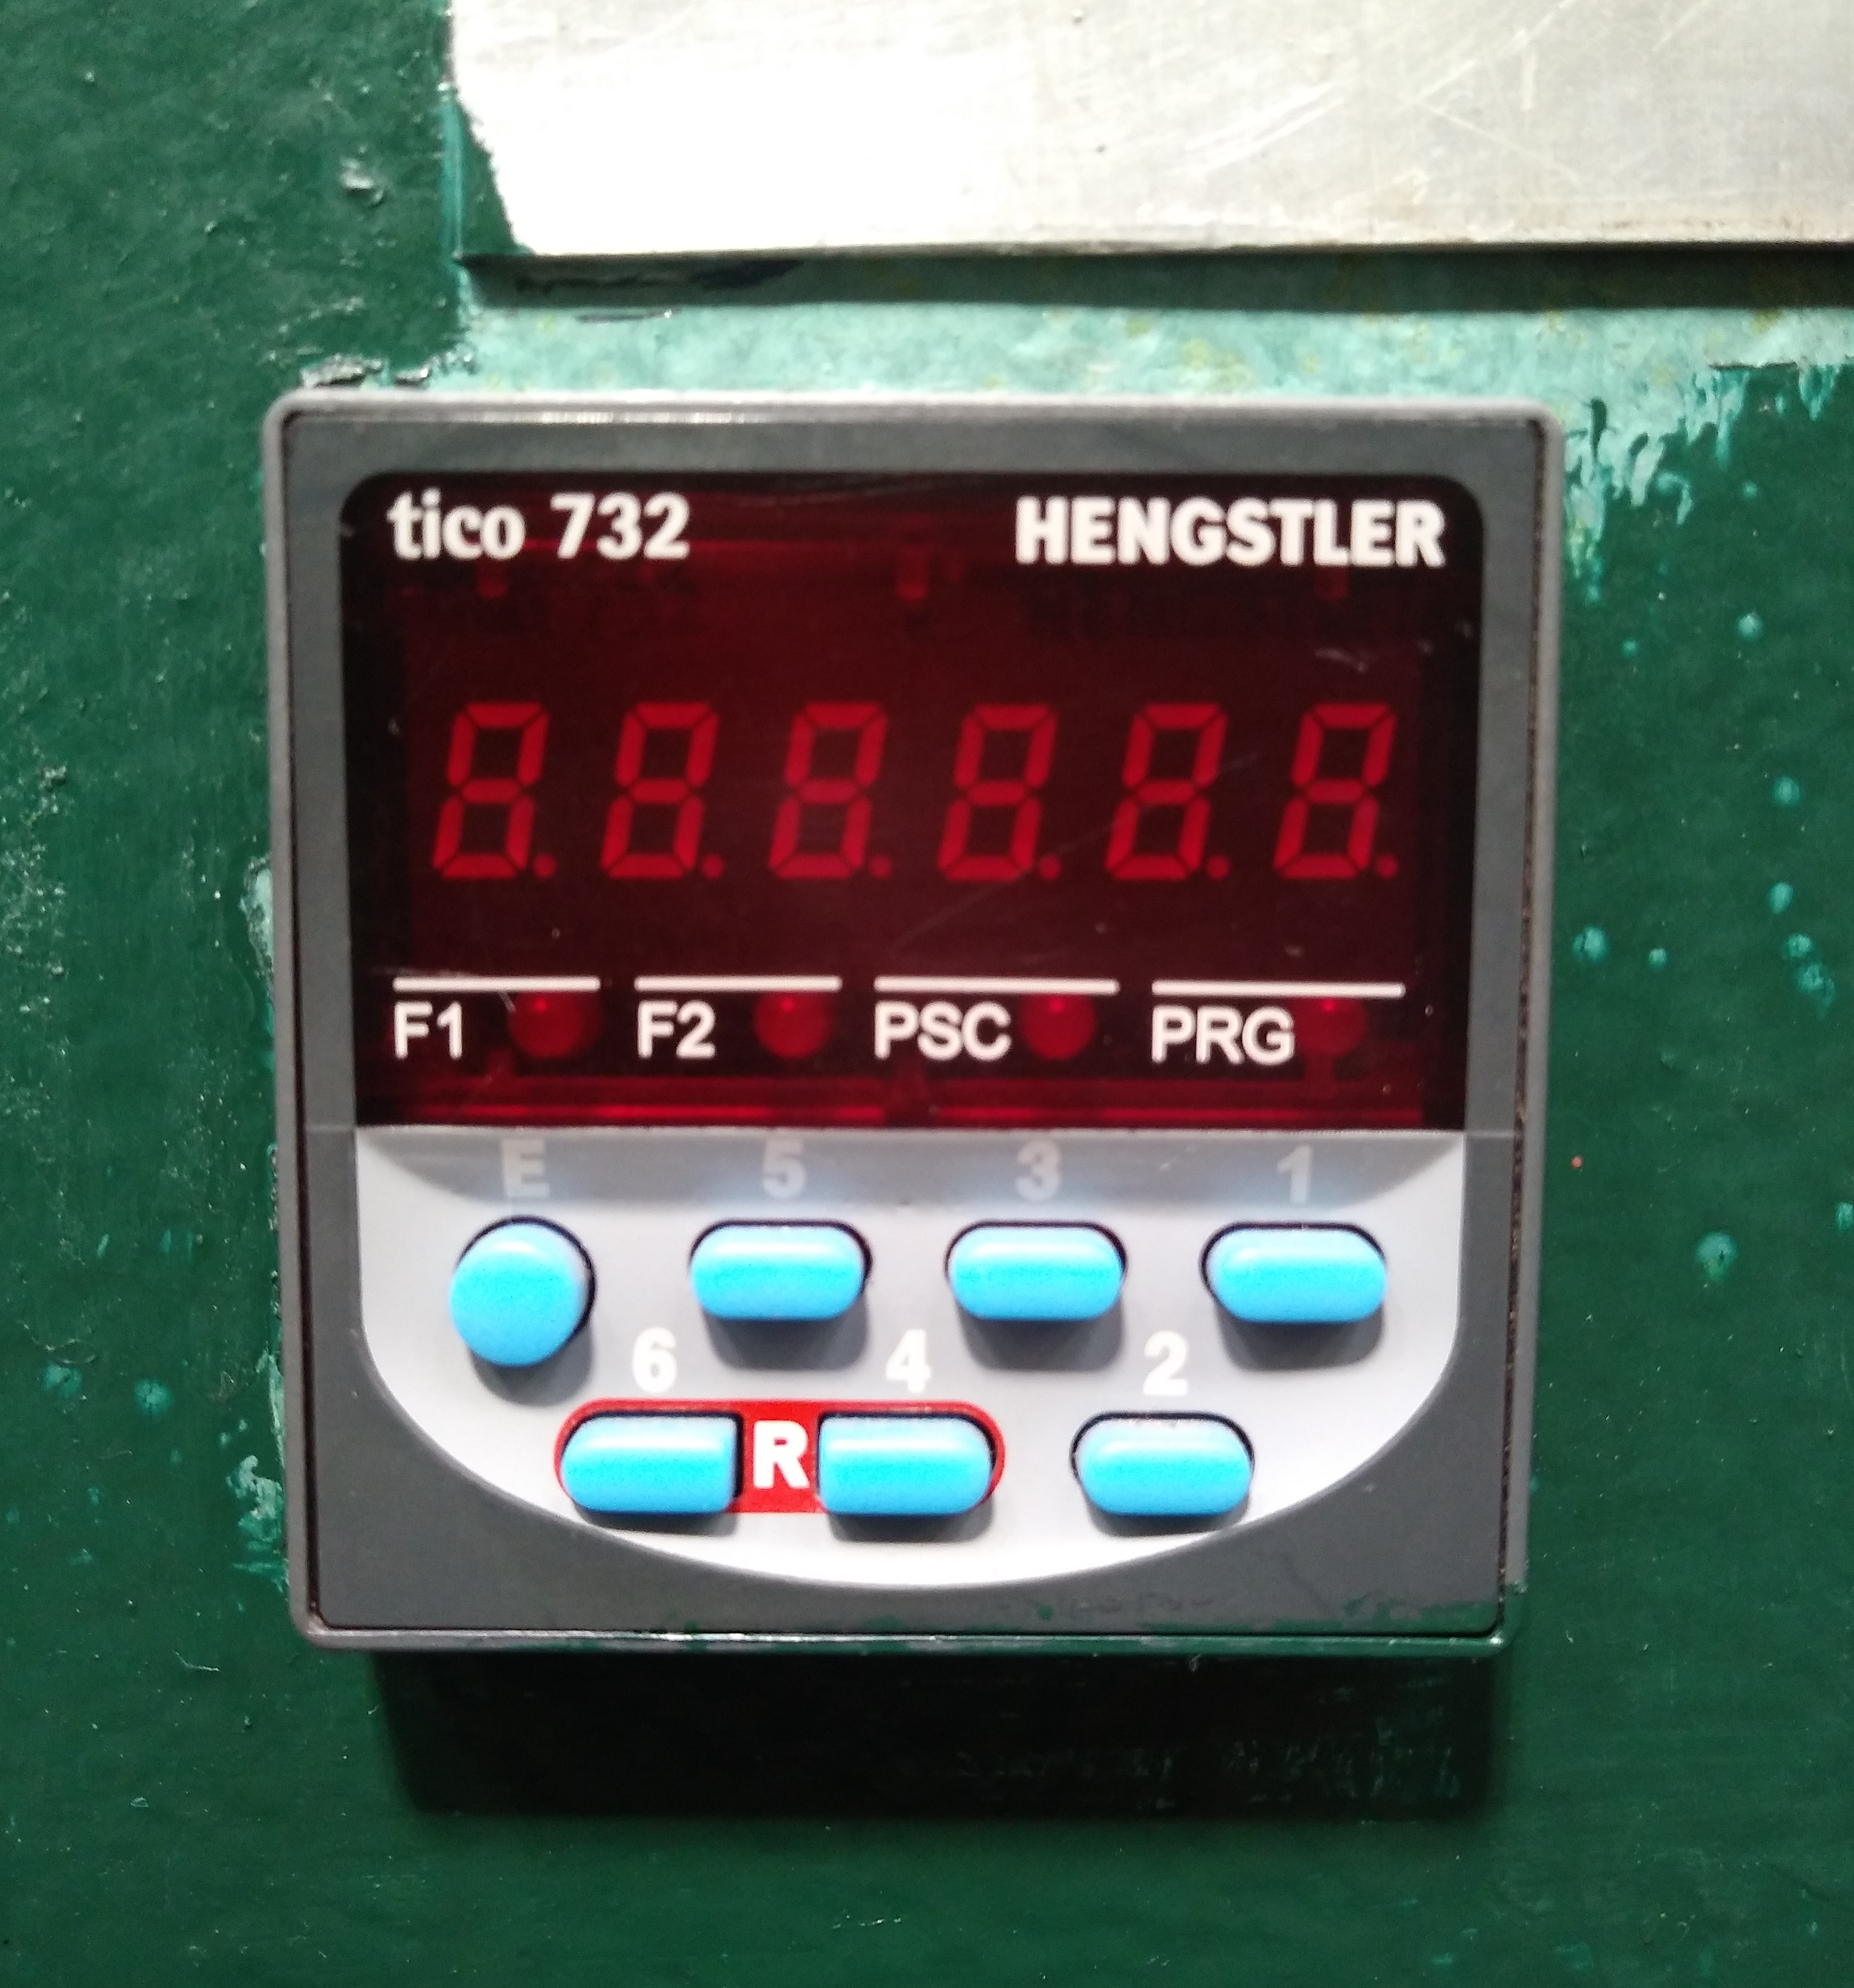
\includegraphics[width=0.4\linewidth]{Imagenes/cont_elect.jpg}
\caption{Control del contador electrónico}
\label{fig:cont_elect}
\end{figure}

El sistema eléctrico de la máquina permanece intacto, el cual se encuentra conectada a la red de la universidad. Conserva su motor eléctrico original junto a un conjunto eléctrico cuya función es suministrar energía de manera continua y estable al motor, para evitar que el ensayo de fatiga se pueda ver afectado por problemas y las variaciones del suministro eléctrico. El motor es de corriente continua con velocidad constante y sus especificaciones se pueden ver en la tabla \ref{tab:motor_maq}.

Otro elemento distinto al original consiste en la correa de transmisión entre el motor eléctrico y el disco desbalanceado. La original consistía en una correa de cuero plana y cruzada, sin información respecto a su empalme. La correa actual consiste también en una correa plana y cruzada, sin embargo, su material es tela y el empalme es realizado a mano con hilo acerado dentro de la misma máquina. Lo particular de estas características dificultan la búsqueda de una correa que pueda cumplir de manera óptima la transmisión de potencia. Esta dificultad se debe a que el sistema de transmisión no ha sido modificado, es decir, sus poleas tienen dimensiones, tanto de diámetro como de ancho, que no están normalizadas o se encuentran fuera de catálogo de mucho proveedores. 

Por otro lado, los elementos de agarre de la probeta no tienen modificaciones conocidas, tanto el brazo que recibe el movimiento como el agarre empotrado a la estructura de la máquina. La fabricación de las probetas utilizadas se realiza en el mismo laboratorio a partir de acero AISI 1020 o 1040, el cual para conseguir las dimensiones de la fig. \ref{fig:probeta} se debe cortar y tornear.

Finalmente, para realizar los ensayos en distintas configuraciones existen distintas masas (fig. \ref{fig:contrapesos}) que desequilibran el disco rotativo, como se verá en la sección \ref{sec:funcionamiento}, y estas combinaciones se especifican en una tabla de cargas (anexo \ref{sec:anexob1}). Sin embargo, se desconoce el origen, y en consecuencia, la fiabilidad de la información contenida en esta tabla.

\subsection{Funcionamiento}
\label{sec:funcionamiento}
La máquina de fatiga tiene como objetivo lograr cargar la probeta de manera cíclica y constante a lo largo de todo el ensayo. Para lograr esto, el mecanismo utilizado es un disco desequilibrado girando a una velocidad constante $\omega_{max}$, la fuerza es transmitida hasta un brazo que sostiene a su vez a la probeta, generando flexión sobre esta con un doble empotramiento. La velocidad $\omega$ del disco se transmite desde el motor eléctrico a través de poleas y una correa de transmisión en una relación de 1:1, a una velocidad de 1500 revoluciones por minuto. Así, para realizar las mediciones de fatiga a distintas cargas se modifica el desequilibrio del disco a través de un conjunto de masas, mostradas en la fig. \ref{fig:contrapesos}, que permiten generar distintas configuraciones y, por consiguiente, esfuerzos en la probeta.

\begin{figure}[h]
\centering
\includegraphics[width=1\linewidth]{Imagenes/contrapesos.jpg}
\caption{Contrapesos utilizados para desequilibrar el disco. De izquiera a derecha se aprecia el n$^{\circ}$ 5 al n$^{\circ}$ 1.}
\label{fig:contrapesos}
\end{figure}

Los elementos utilizados para desbalancear son 6 discos pequeños, enumerados del 1 al 5, donde el 1 es el más liviano y el 5 el más pesado, todos de distinto peso y el quinto se encuentra repetido. Estas se colocan en el perímetro del disco giratorio de forma diametralmente opuesta, como se ve en la fig. \ref{fig:disco_post}, dependiendo de la carga que se desee generar. Para conocer que configuración corresponde a cada esfuerzo aplicado sobre la probeta se utiliza la tabla de cargas.

\begin{figure}[h]
\centering
	\begin{subfigure}{0.32\linewidth}
		\centering
		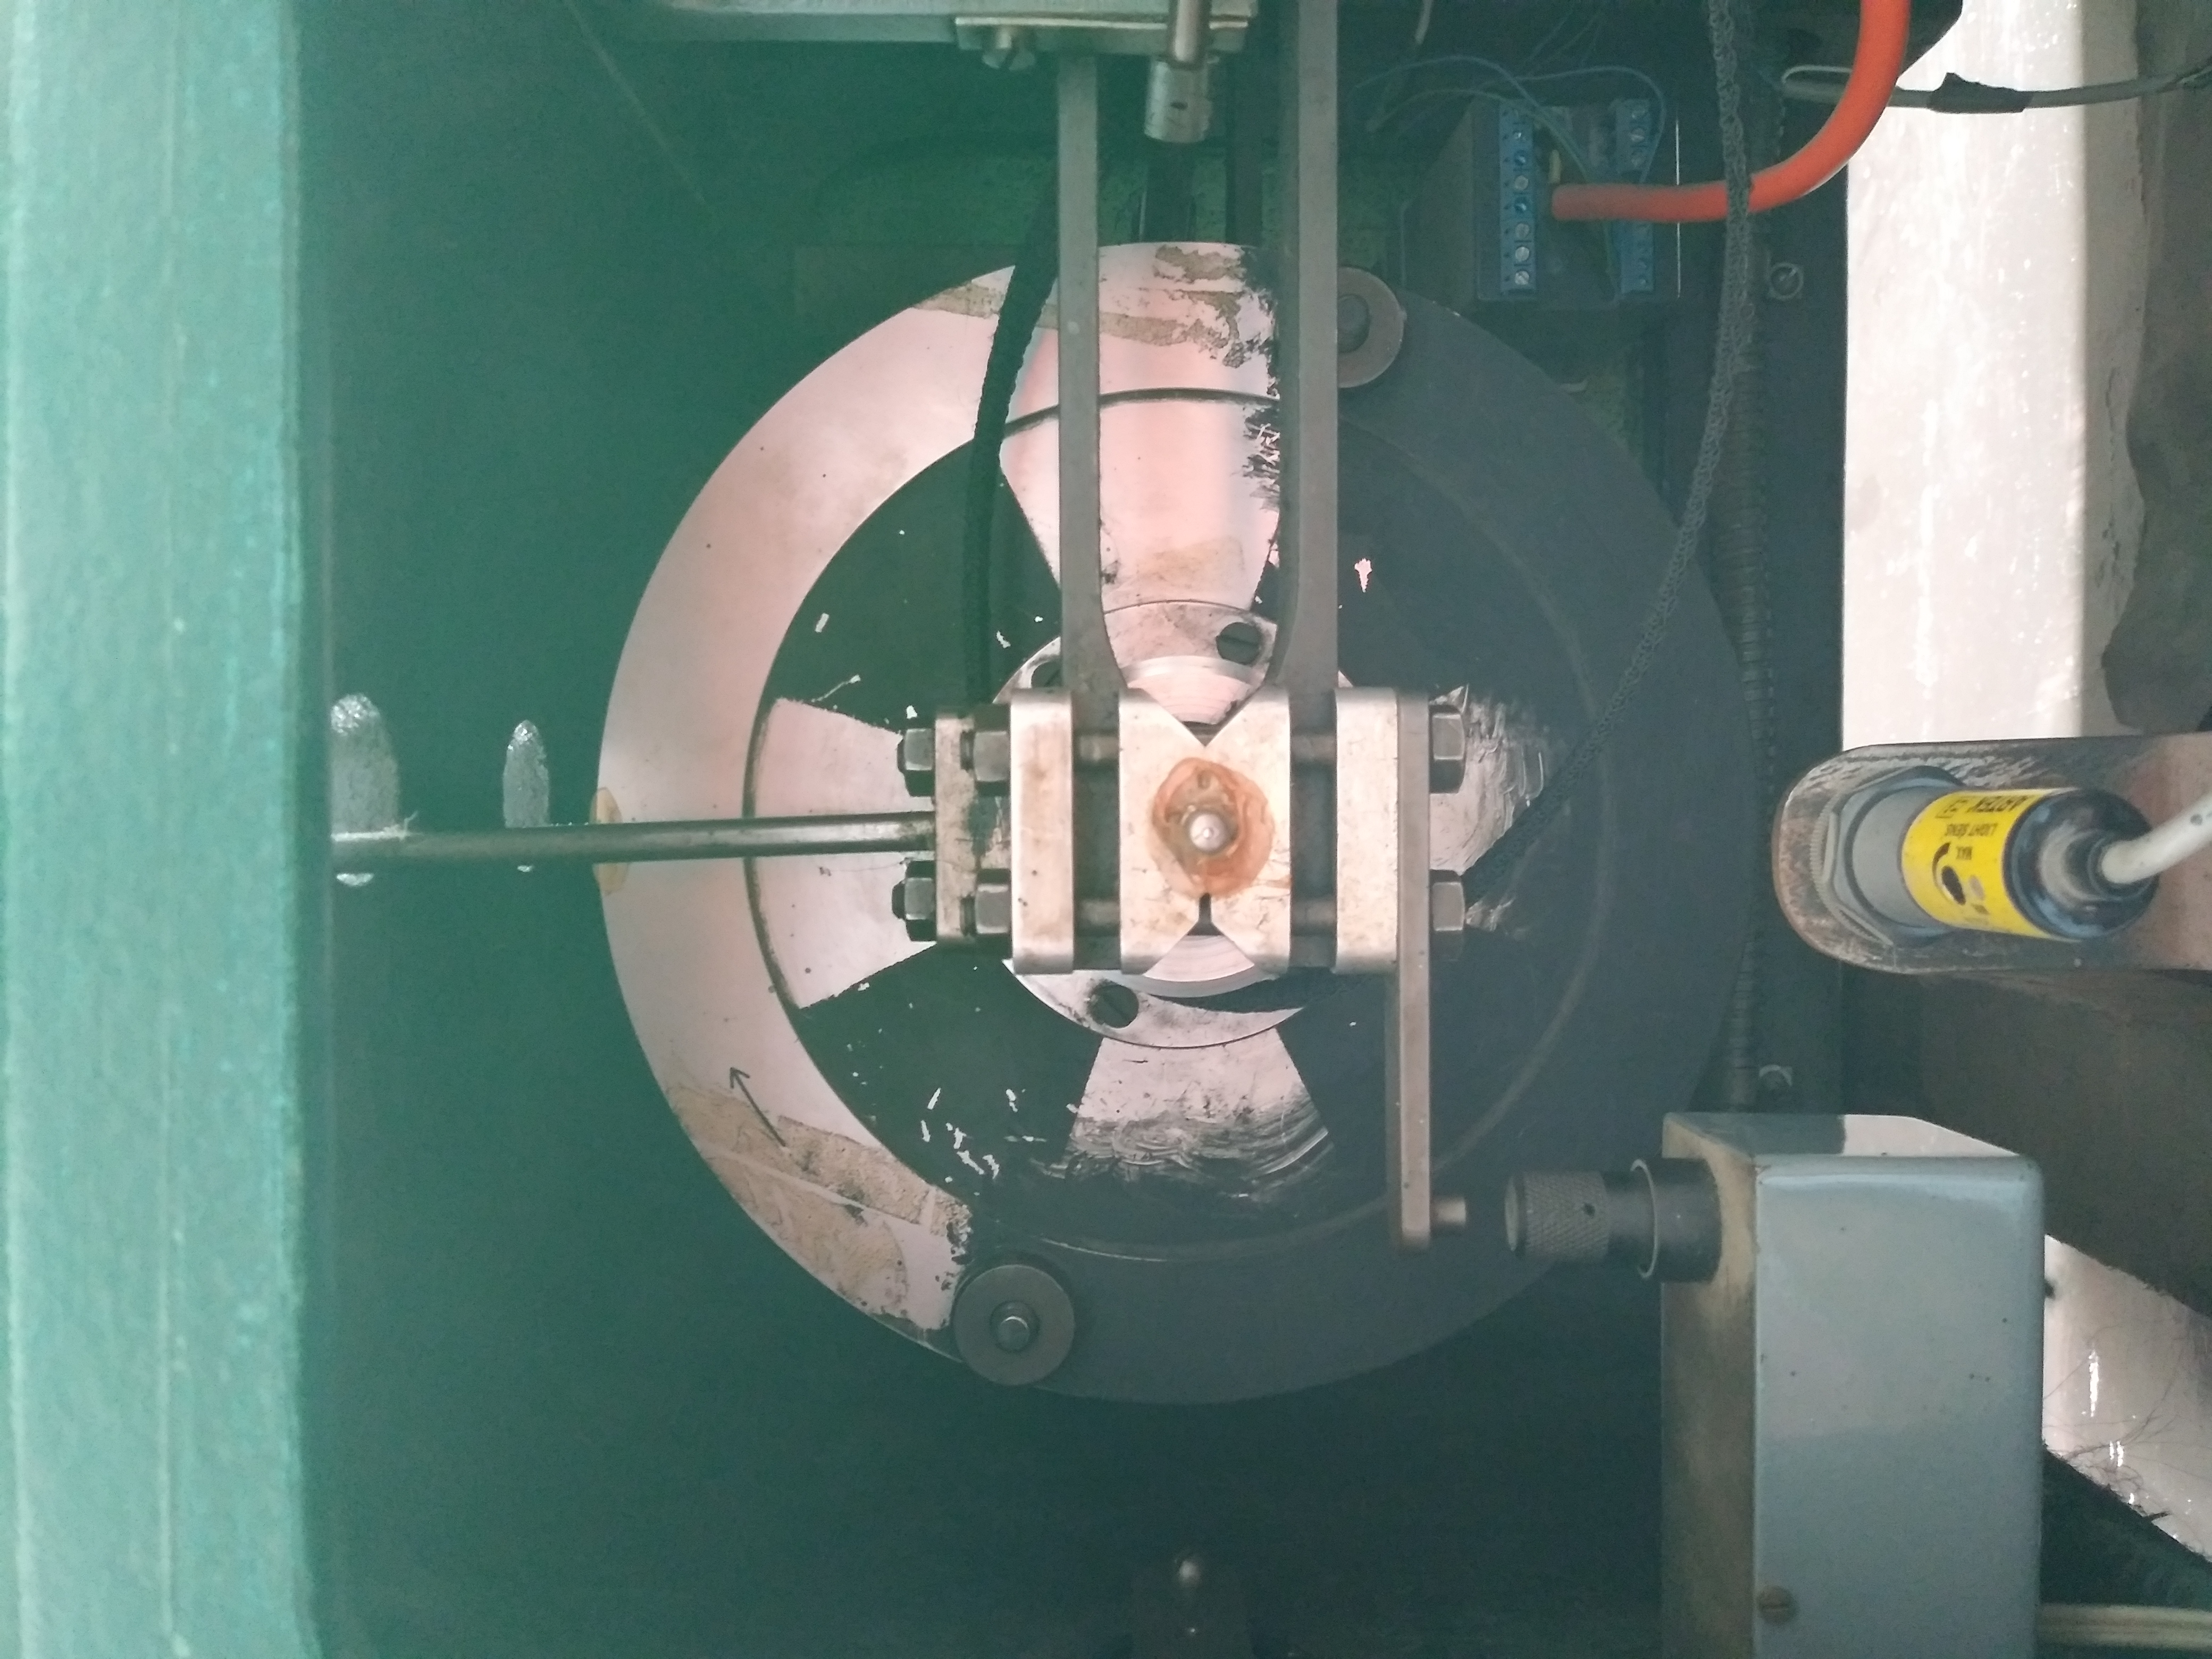
\includegraphics[angle=270, origin=c, width=\linewidth]{Imagenes/disco_anterior.jpg}
		\caption{Vista delantera.}\label{fig:disco_ant}
	\end{subfigure}
	\begin{subfigure}{0.32\linewidth}
		\centering
		\includegraphics[angle=270, origin=c, width=\linewidth]{Imagenes/disco_posterior.jpg}
		\caption{Vista anterior.}\label{fig:disco_post}
	\end{subfigure}
		\begin{subfigure}{0.32\linewidth}
		\centering
		\includegraphics[angle=270, origin=c, width=\linewidth]{Imagenes/disco_lateral.jpg}
		\caption{Vista lateral.}\label{fig:disco_lat}
	\end{subfigure}%
\caption{Distintas vistas del disco desbalanceado de la máquina. En la imagen (b) se pueden apreciar claramente los soportes de los contrapesos en los extremos del disco, en cambio, en la imagen (c) se ven los distintos componentes que están adosados al disco.}
\label{fig:disco_completo}
\end{figure}

Esta tabla, con 3 columnas de información como se ve en el anexo \ref{sec:anexob1}, nos entrega el esfuerzo $\sigma$, cortante $\tau$ y la combinación necesaria para generar esos esfuerzos. Los números entre paréntesis nos indican cuantos contrapesos se deben apilar en cada perno adosado al disco giratorio, los cuales llamaremos soportes de contrapeso. Así, la tabla nos señala que la fuerza es función de la diferencia de masa entre cada soporte, es decir, la suma de las masas de cada paréntesis. A modo de ejemplo, en la tabla \ref{tab:ejemplo_config} se han colocado las 4 primeras filas de la tabla de cargas, añadiendo 4 columnas a la derecha de ``Combinación'' con información sobre el peso de cada una. En las columnas $m_1$ y $m_2$ se aprecia la suma de cada masa colocada en sus soportes de contrapeso señalado por la columna de ``Combinación''. Las columnas siguientes representan $\Delta m = m_1-m_2$ y $m_{total}=m_1+m_2$. Como se puede apreciar, los esfuerzos normales y cortantes aumentan en la medida que $\Delta m$ de cada combinación aumenta, independiente de $m_{total}$.

\begin{table}[h]
\centering
\begin{tabular}{@{}cclllll@{}}
\toprule
$\sigma \left[\frac{\text{kg}_f}{\text{cm}^2}\right]$ & {$\tau \left[\frac{\text{kg}_f}{\text{cm}^2}\right]$} & Combinación     & $m_1$ {[}g{]} & $m_2$ {[}g{]} & $\Delta m$ {[}g{]} & $m_{total}$ {[}g{]} \\ \midrule
40                                                   & 20                                                                    & (5) - (1+2+3+4) & 30,9199       & 30,5071       & 0,4128             & 61,427              \\
80                                                   & 40                                                                    & (1) - (0)       & 0,7582        & 0             & 0,7582             & 0,7582              \\
120                                                  & 60                                                                    & (5) - (4+2+3)   & 30,9199       & 29,7489       & 1,171              & 60,6688             \\
160                                                  & 80                                                                    & (2) - (1)       & 2,2969        & 0,7582        & 1,5387             & 3,0551              \\ \bottomrule
\end{tabular}
\caption{Tabla de cargas modificada, mostrando el peso de cada combinación, su diferencia y el total.}
\label{tab:ejemplo_config}
\end{table}

Con esto, la probeta a ensayar estará sometida a un esfuerzo en flexión, empotrada por la mordaza del brazo de carga y la mordaza empotrada a la estructura de la máquina, ambas mostradas en la fig. \ref{fig:mordazas}.

\begin{figure}[h]
\centering
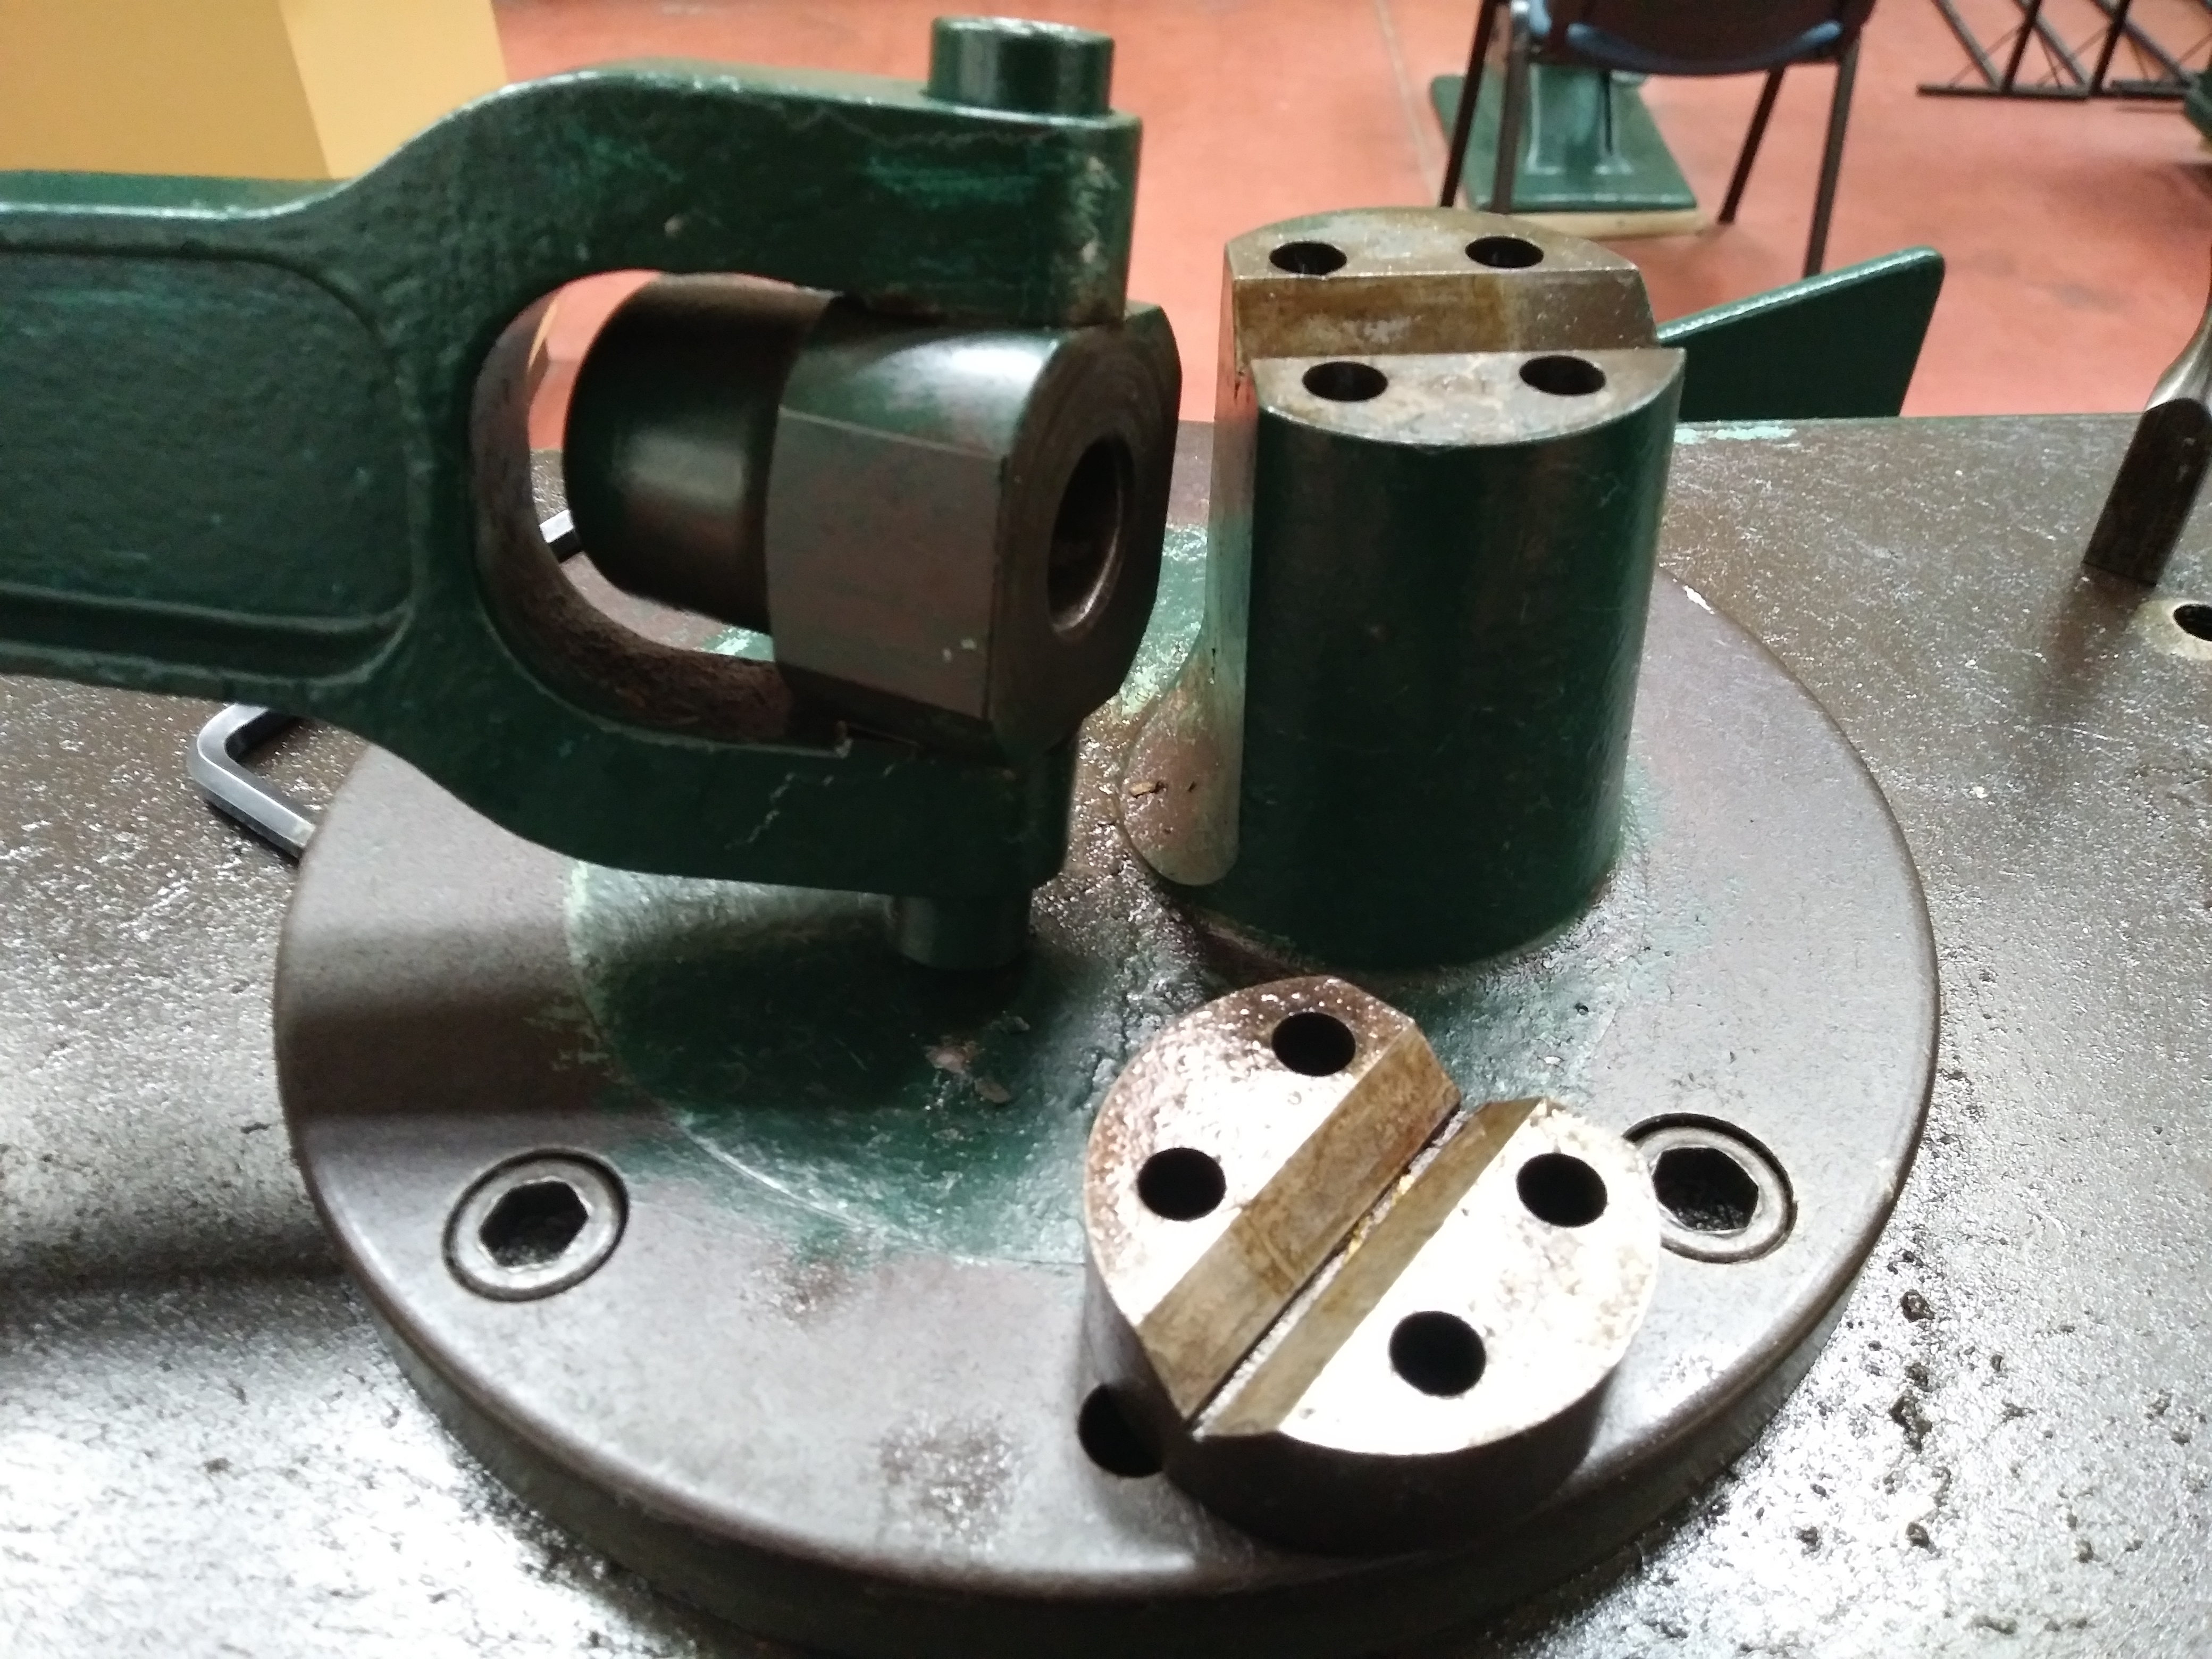
\includegraphics[width=0.8\linewidth]{Imagenes/mordazas.jpg}
\caption{A la izquierda se aprecia la mordaza de la barra de carga, a la derecha la mordaza empotrada sin la parte superior y apoyada sobre esta, la probeta.}
\label{fig:mordazas}
\end{figure}

Una vez que se haya escogido la configuración de masas y la probeta se encuentre en su posición, una pequeña barra de bloqueo con una manilla ubicada entre las barras de acero, como se aprecia en la fig. \ref{fig:barra_bloqueo}, eleva ambas barras con el objetivo de evitar que oscile en su frecuencia natural durante el encendido y aceleración del motor hasta su velocidad final, dejando a la barra en una configuración de empotrado y apoyo simple. Una vez que el motor alcanza una velocidad estable, el sostén es girado nuevamente para dejar al disco giratorio en posición de empotrado-libre. Este sostén, permite que el ensayo de fatiga se realice siempre a una frecuencia constante y evitar la transición inicial del motor. Una vez que la probeta se fracture, provocará un aumento en la amplitud de las oscilaciones del disco las cuales activarán el freno automático (fig. \ref{fig:freno_auto}) para detener el motor y, por lo tanto, el ensayo. Gracias a este sistema, es posible conocer la cantidad de ciclos realizados hasta el momento de la fractura sin la necesidad de supervisar de manera continua el ensayo.

\begin{figure}[h]
\centering
	\begin{subfigure}{0.55\linewidth}
		\centering
		\includegraphics[width=\linewidth]{Imagenes/freno_automatico.jpg}
		\caption{Freno automático.}\label{fig:freno_auto}
	\end{subfigure}
	\begin{subfigure}{0.365\linewidth}
		\centering
		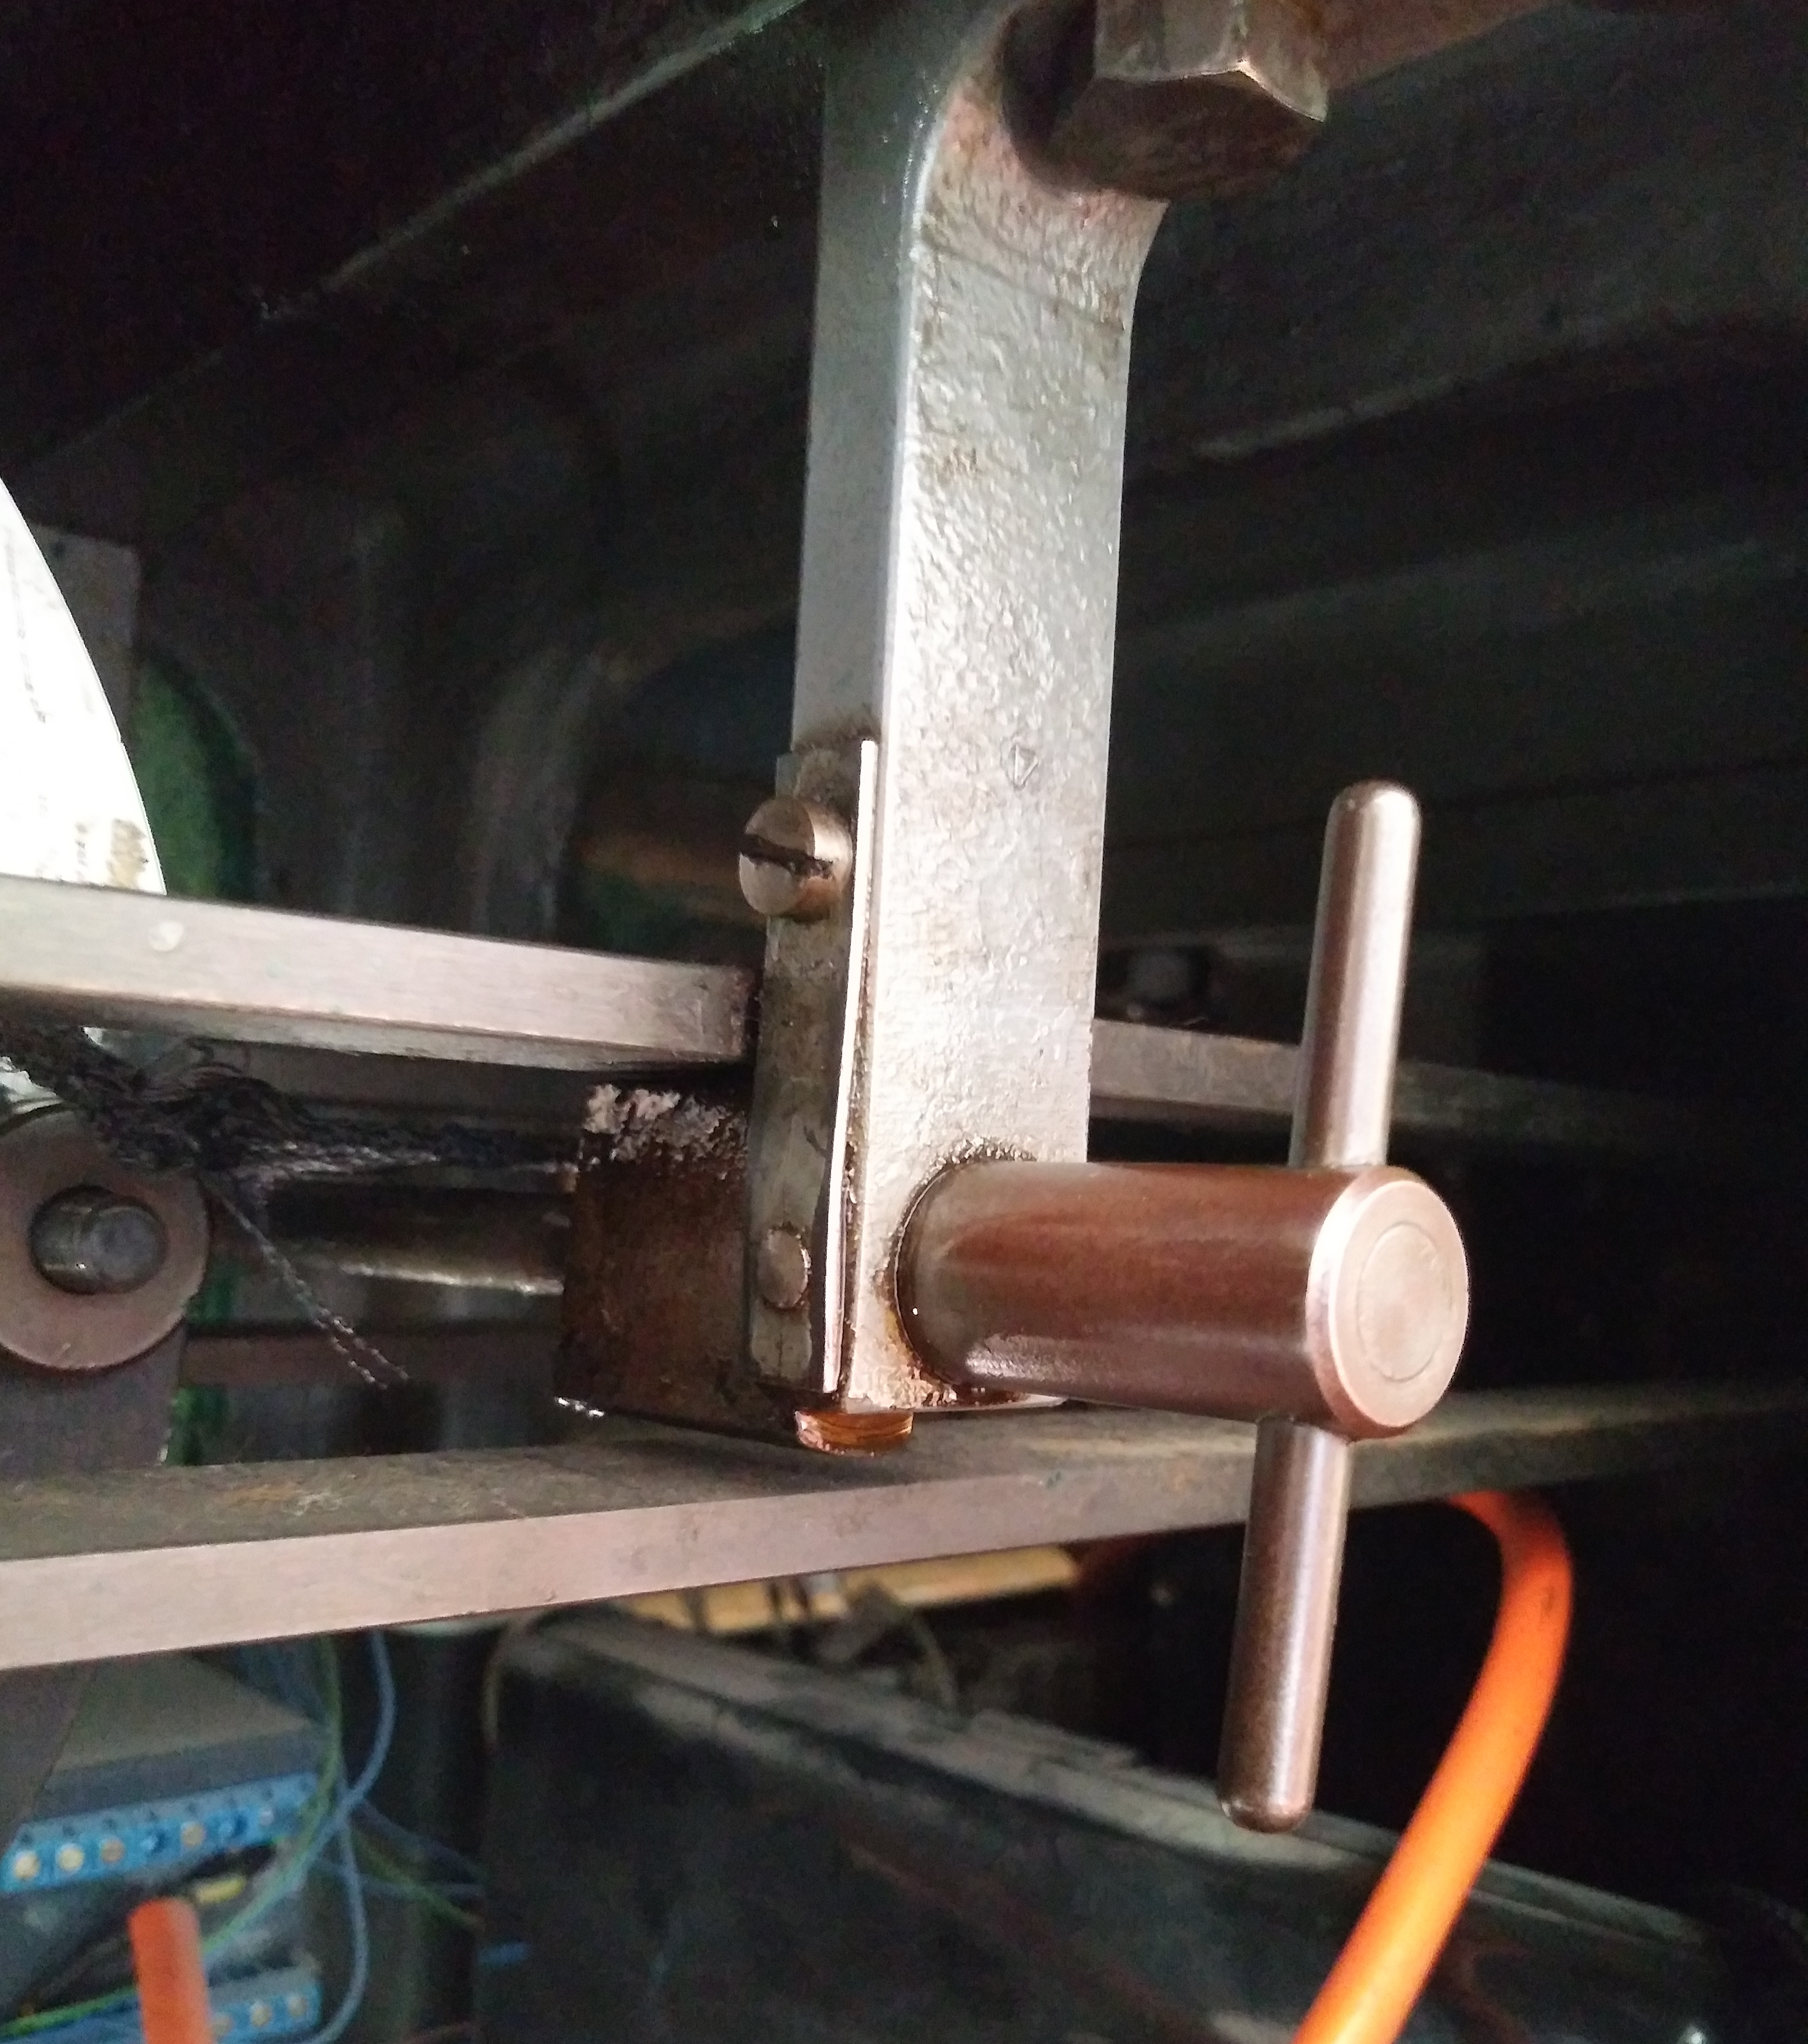
\includegraphics[width=\linewidth]{Imagenes/barra_bloqueo.jpg}
		\caption{Barra de bloqueo.}\label{fig:barra_bloqueo}
	\end{subfigure}%
\caption{En la imagen (a) se aprecia el botón del freno automático y la extensión que lo presiona. En la imagen (b) la barra de bloqueo sosteniendo las vigas en voladizo.}
\label{fig:barra_freno}
\end{figure}

\subsection{Mediciones}
\label{sec:mediciones_met}
Para realizar un correcto diseño de la estructura soportante y la comprensión de su funcionamiento, se hace vital poder contar con información confiable para obtener resultados correctos. Para esto, las mediciones se dividirán según su objetivo en el desarrollo de este trabajo.
\subsubsection{Diseño de estructura}
Las medidas de la mesa actual son: 
\begin{itemize*}
	\item Ancho = 74,5 cm
	\item Largo = 177 cm
	\item Altura = 91 cm
\end{itemize*}
Por otro lado, para diseñar correctamente la estructura se deben conocer las dimensiones de la máquina, su peso y la ubicación de los pernos de anclaje, así como también el tipo de perno utilizado. La fig. \ref{fig:diag_maqfat} es un esquema representativo de la máquina, mostrando sus dimensiones de ancho, alto y largo, las dimensiones de su base y la ubicación de sus pernos. La masa de toda la máquina se aproximó a partir de las dimensiones externas, estimando el grosor de sus paredes y considerando el peso específico del acero fundido, sobrestimando el valor del espesor de sus paredes como factor de seguridad. Considerando el peso específico del acero $\rho_{acfund} = 7850 \, [Kg/m^3]$, entonces la masa total calculada es:

\[ \left. 
\begin{array}{ll}
V_{base} &= (3,3\cdot 91\cdot 39 - 3\cdot 88\cdot 37)\; \text{cm}^3	\\
V_{superior} &=(30,2\cdot 84\cdot 32 - 26\cdot 78\cdot 28,5) \; \text{cm}^3	\\
\end{array}
\right\} \\
\quad V_{b+s} = 25323,3 \; \text{cm}^3 \]
\begin{equation}\label{eq:masa_maq}
	m_{maq} = \rho_{ac. fundido} \cdot V_{b+s} = 198,8 \: kg \approx 200 \: kg
\end{equation}

\begin{figure}[h]
\centering
\includegraphics[width=1\linewidth, trim={10cm 37cm 17cm 2cm},clip]{Imagenes/MaqFatiga-1.pdf}
\caption{Esquema de la máquina de fatiga y sus dimensiones externas, en mm.}
\label{fig:diag_maqfat}
\end{figure}

\subsubsection{Componentes de la máquina de fatiga}
\subparagraph{Sistema de transmisión.}
El sistema de transmisión está compuesto por el motor eléctrico, cuyas características se detallaron anteriormente, la correa de transmisión y ambas poleas. Las dimensiones y características de las poleas conductora y conducida, como también de la correa se encuentran en la tabla \ref{tab:sist_transmision}. 

\begin{table}[h]
\centering
\begin{tabular}{@{}ll@{}}
\toprule
Características          & Valor   			\\ \midrule
Diámetro polea motriz    & 48 mm   			\\
Diámetro polea conducida & 47,5 mm 			\\
Relación de poleas		 & $\approx$ 1 (-) 	\\
Ancho correa             & 10 mm   			\\
Longitud correa          & 1235 mm 			\\
Configuración            & Cruzada 			\\ \bottomrule
\end{tabular}
\caption{Datos del sistema de transmisión}
\label{tab:sist_transmision}
\end{table}

\subparagraph{Sistema de vigas en voladizo}
El conjunto de barras en voladizo que sostienen el disco en empotrado-libre, tienen medidas levemente distintas para las superiores respecto a las inferiores, separadas por una distancia de 32 mm. La tabla \ref{tab:medidas_barrasacero} muestra las medidas de cada una.
\begin{table}[h]
\centering
\begin{tabular}{@{}lll@{}}
\toprule
Medida  & Barras superiores {[}mm{]} & Barras inferiores {[}mm{]} \\ \midrule
Espesor      & 5,7                        & 5,8                        \\
Ancho        & 25,1                       & 25,2                       \\
Largo        & 333                        & 333                        \\ \bottomrule
\end{tabular}
\caption{Medidas de las vigas en voladizo según su posición}
\label{tab:medidas_barrasacero}
\end{table}

Con estos datos, es posible calcular el segundo momento de área respecto a un eje central horizontal equidistante entre las barras superiores e inferiores, según el cual se obtiene $\bar{I}_{barras}=$ 5,67$\cdot$ 10$^{-8} \text{ m}^4$. 

\subparagraph{Sistema de transmisión de fuerzas.}
El brazo principal (fig. \ref{fig:brazo_carga}) que ejerce la fuerza sobre la probeta proveniente del disco desbalanceado, está constituido por tres partes principales. La primera de ellas es la parte trasera, con forma regular rectangular, está hecho de una aleación de aluminio y dos tercios de su longitud es ahuecada. La segunda y principal, está hecha de acero fundido y añade el mayor porcentaje de masa al total del brazo. Finalmente, la última parte consiste en la mordaza, unida a la sección principal con dos pernos que permiten ajustar su posición. La longitud total del brazo es de 359 mm y su masa total 2,305 kg.

\begin{figure}[h]
\centering
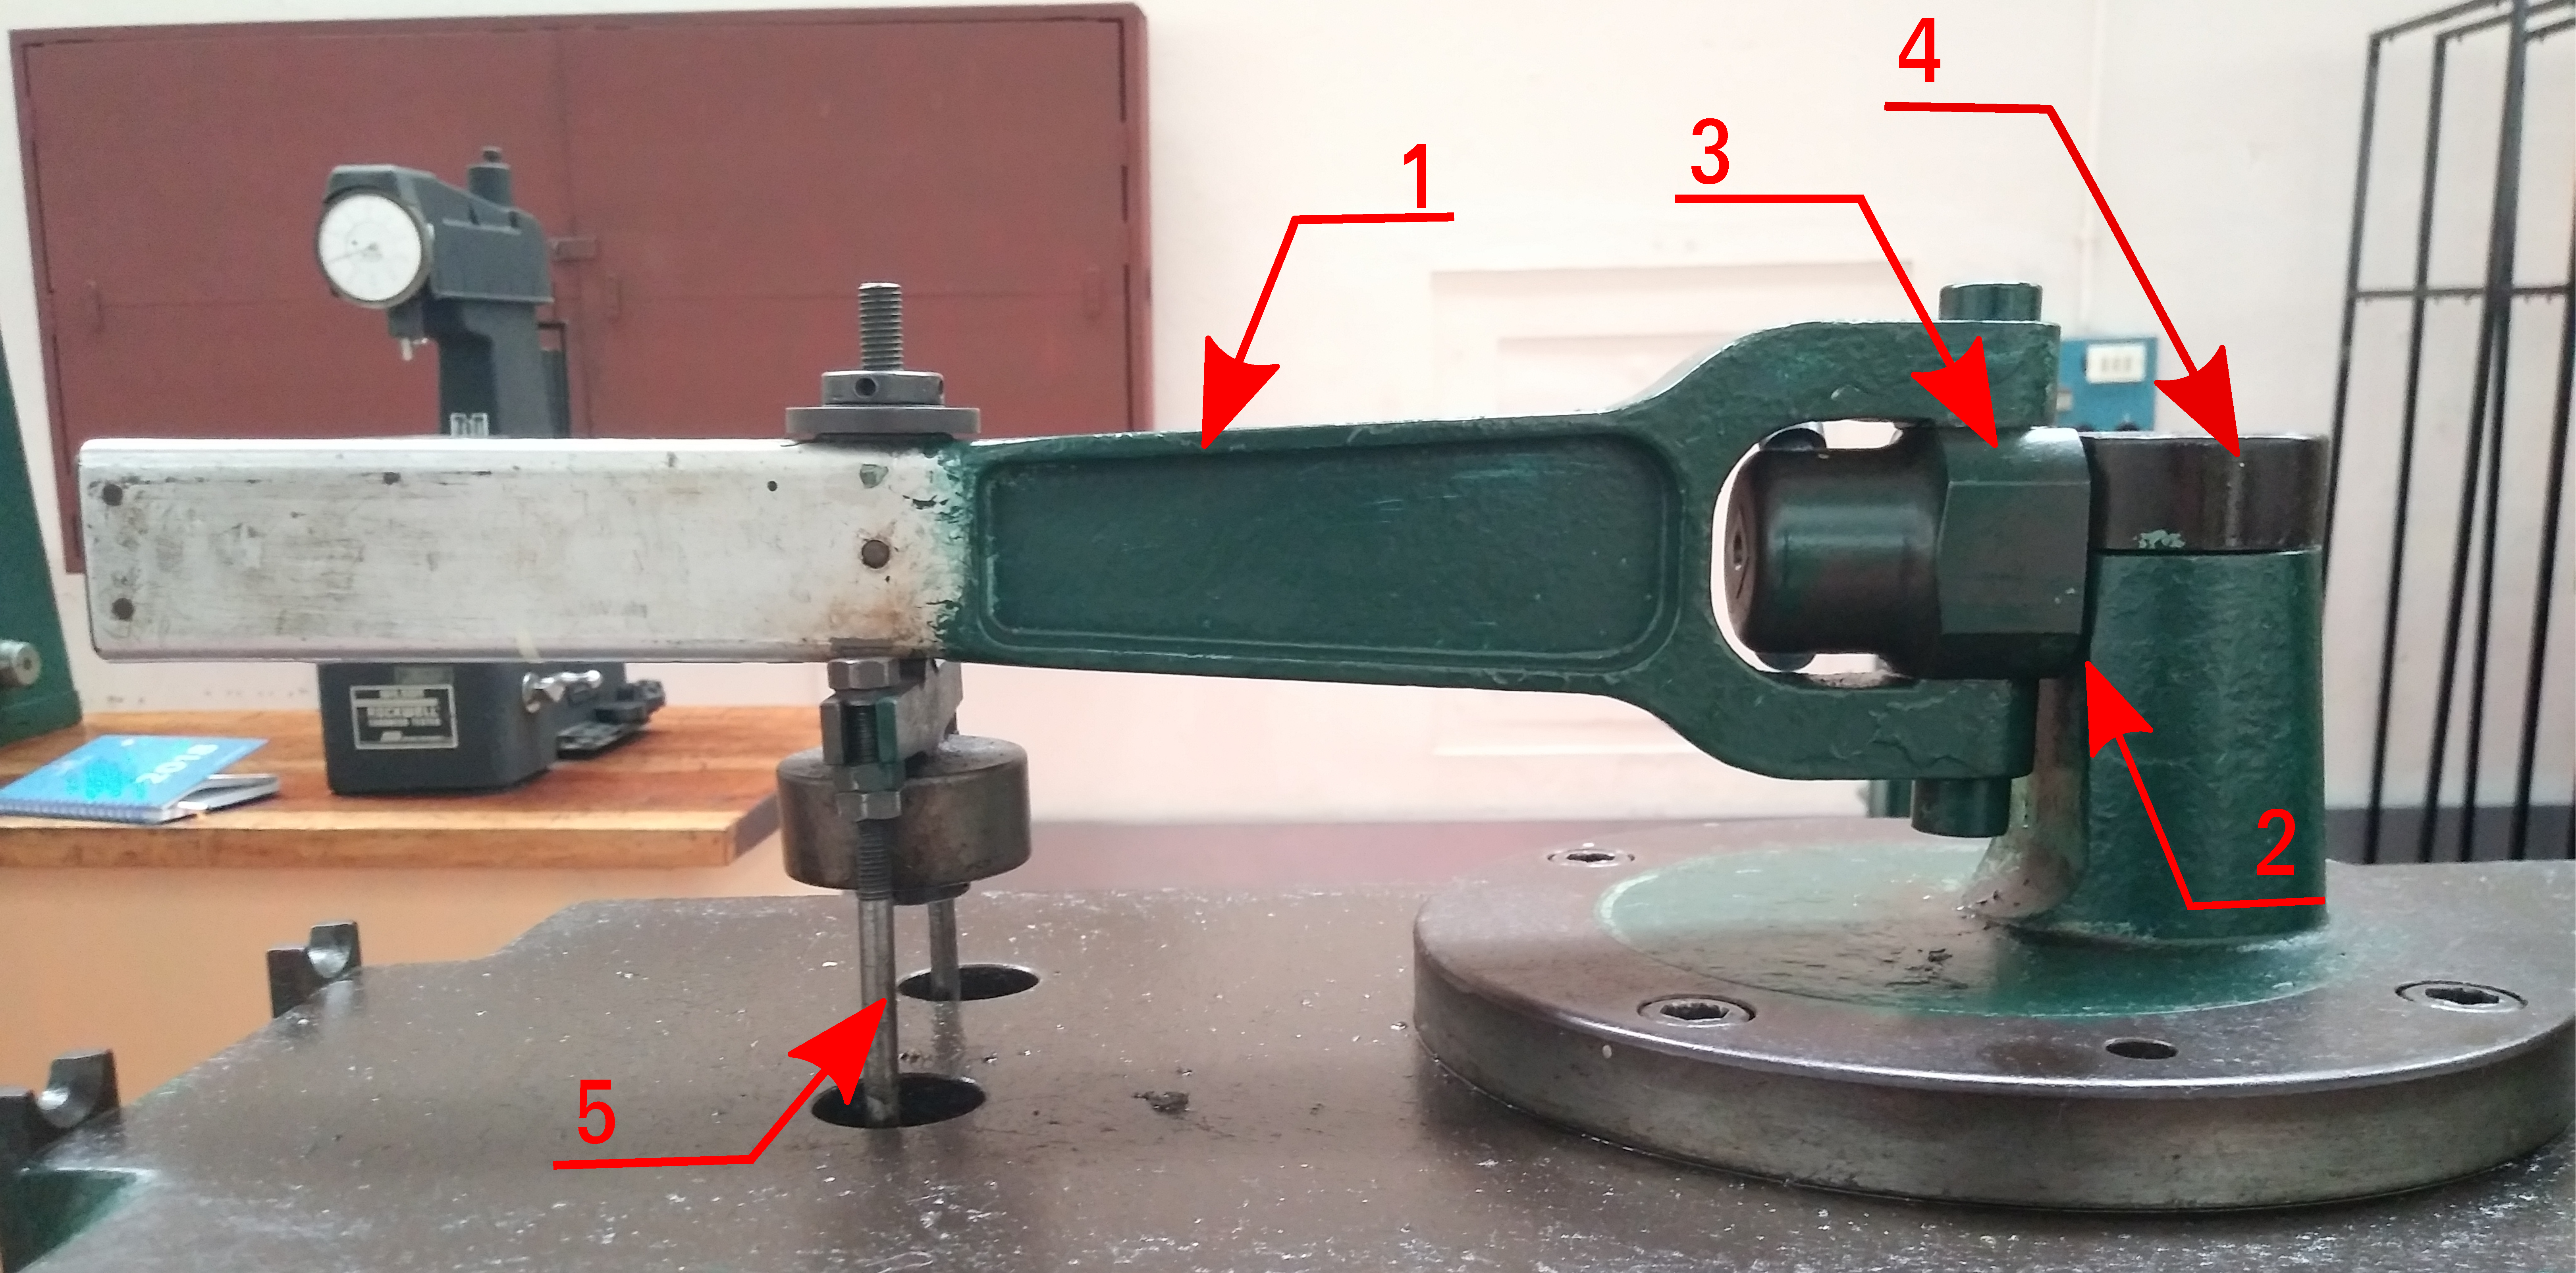
\includegraphics[width=0.9\linewidth]{Imagenes/brazo_carga.jpg}
\caption{Brazo de carga junto a su mordaza y la mordaza empotrada a la derecha.}
\label{fig:brazo_carga}
\end{figure}

La transmisión de la carga entre el disco desbalanceado y el brazo de carga se da a través de dos barras de acero redondas, uno a cada lado del disco, de diámetro 6,2 mm y largo de 169 mm.

\subparagraph{Disco desbalanceado y contrapesos.}
En base a las características visuales y auditivas del disco, se cree que está construido de alguna aleación de aluminio. Su radio $R_d =$ 112 mm y espesor de 6,4 mm. 

La masa de cada contrapeso (fig. \ref{fig:contrapesos}) fue medida en el laboratorio de ingeniería metalúrgica con una balanza analítica.
\begin{table}[H]
\centering
\begin{tabular}{@{}cccc@{}}
\toprule
Contrapeso & Masa {[}g{]}	& Diámetro {[}mm{]}	&	Espesor promedio {[}mm{]} \\ \midrule
1          & 0,7582			& 20,55				&	1,00	         		  \\
2          & 2,2969       	& 27,00				&	1,50					  \\
3          & 6,8541       	& 27,00				& 	1,70	 		   		  \\
4          & 20,5979      	& 27,90				& 	5,00			 		  \\
5          & 30,9199      	& 29,90				&	4,40			 		  \\ \bottomrule
\end{tabular}
\caption{Masa de cada contrapeso utilizado}
\label{tab:masa_contrapesos}
\end{table}

Por otra parte, no fue posible medir directamente la masa del disco al no poder desarmarlo ni separarlo de su eje. Por lo tanto, se midió de la flecha de la viga en voladizo producida por la masa del disco, la polea, el sistema de sujeción y las barras de acero, para obtener la masa aproximada del disco. Sin embargo, si bien se restó la fuerza producida por la masa de las barras, se incluyó en el cálculo el resto de los elementos acompañantes del disco en la masa obtenida.

\subparagraph{Probeta.} La probeta utilizada actualmente para el ensayo de fatiga es de acero. Su geometría, como se aprecia en la fig. \ref{fig:probeta}, consiste en una pequeña viga de largo 3\nicefrac{1}{2}'', de sección cuadrada en sus extremos y una entalladura en el medio de sección circular, de lado \nicefrac{1}{2}'' de lado y 0,3'' de diámetro respectivamente.
 
\begin{figure}[H]
\centering
\includegraphics[width=1\linewidth, trim={2cm 13cm 4cm 1cm},clip]{Imagenes/Probeta.pdf}
\caption{Vista en corte, lateral y frontal de la probeta con sus respectivas dimensiones.}
\label{fig:probeta}
\end{figure} 
 
\subparagraph{Motor y sistema eléctrico.}
Como se señaló, el motor eléctrico con el que funciona la máquina de fatiga es de corriente continua y sus características se encuentran en la tabla \ref{tab:motor_maq}. El motor tiene una velocidad angular constante, aunque como consecuencia de su antigüedad y tipo de motor, añadirle un variador de frecuencia se vuelve más complejo que cambiar el motor mismo. 

\begin{table}[h]
\centering
\begin{tabular}{ll}
\hline
Especificaciones Motor                            & Valor   				\\ \hline
Tensión                                           & 220 {[}V{]}        		\\
Corriente                                         & 0,8 {[}A{]}        		\\
Factor de potencia ($\cos \varphi$)				  & Sin información    		\\
Potencia                                          & 100 {[}W{]}        		\\
Velocidad                                         & 1500 {[}rev/min{]} 		\\ \hline
\end{tabular}
\caption{Especificaciones del motor de la máquina de fatiga.}
\label{tab:motor_maq}
\end{table}
 
Por otro lado, el sistema eléctrico que se ve en la imagen \ref{fig:sist_elec}, tienen como función en mantener el suministro eléctrico del motor estable. Ahora bien, su tecnología es compleja y se encuentra obsoleta, lo que vuelve difícil mantener, reparar o actualizar sus componentes.

\begin{figure}[h]
\centering
	\begin{subfigure}{0.5\linewidth}
		\centering
		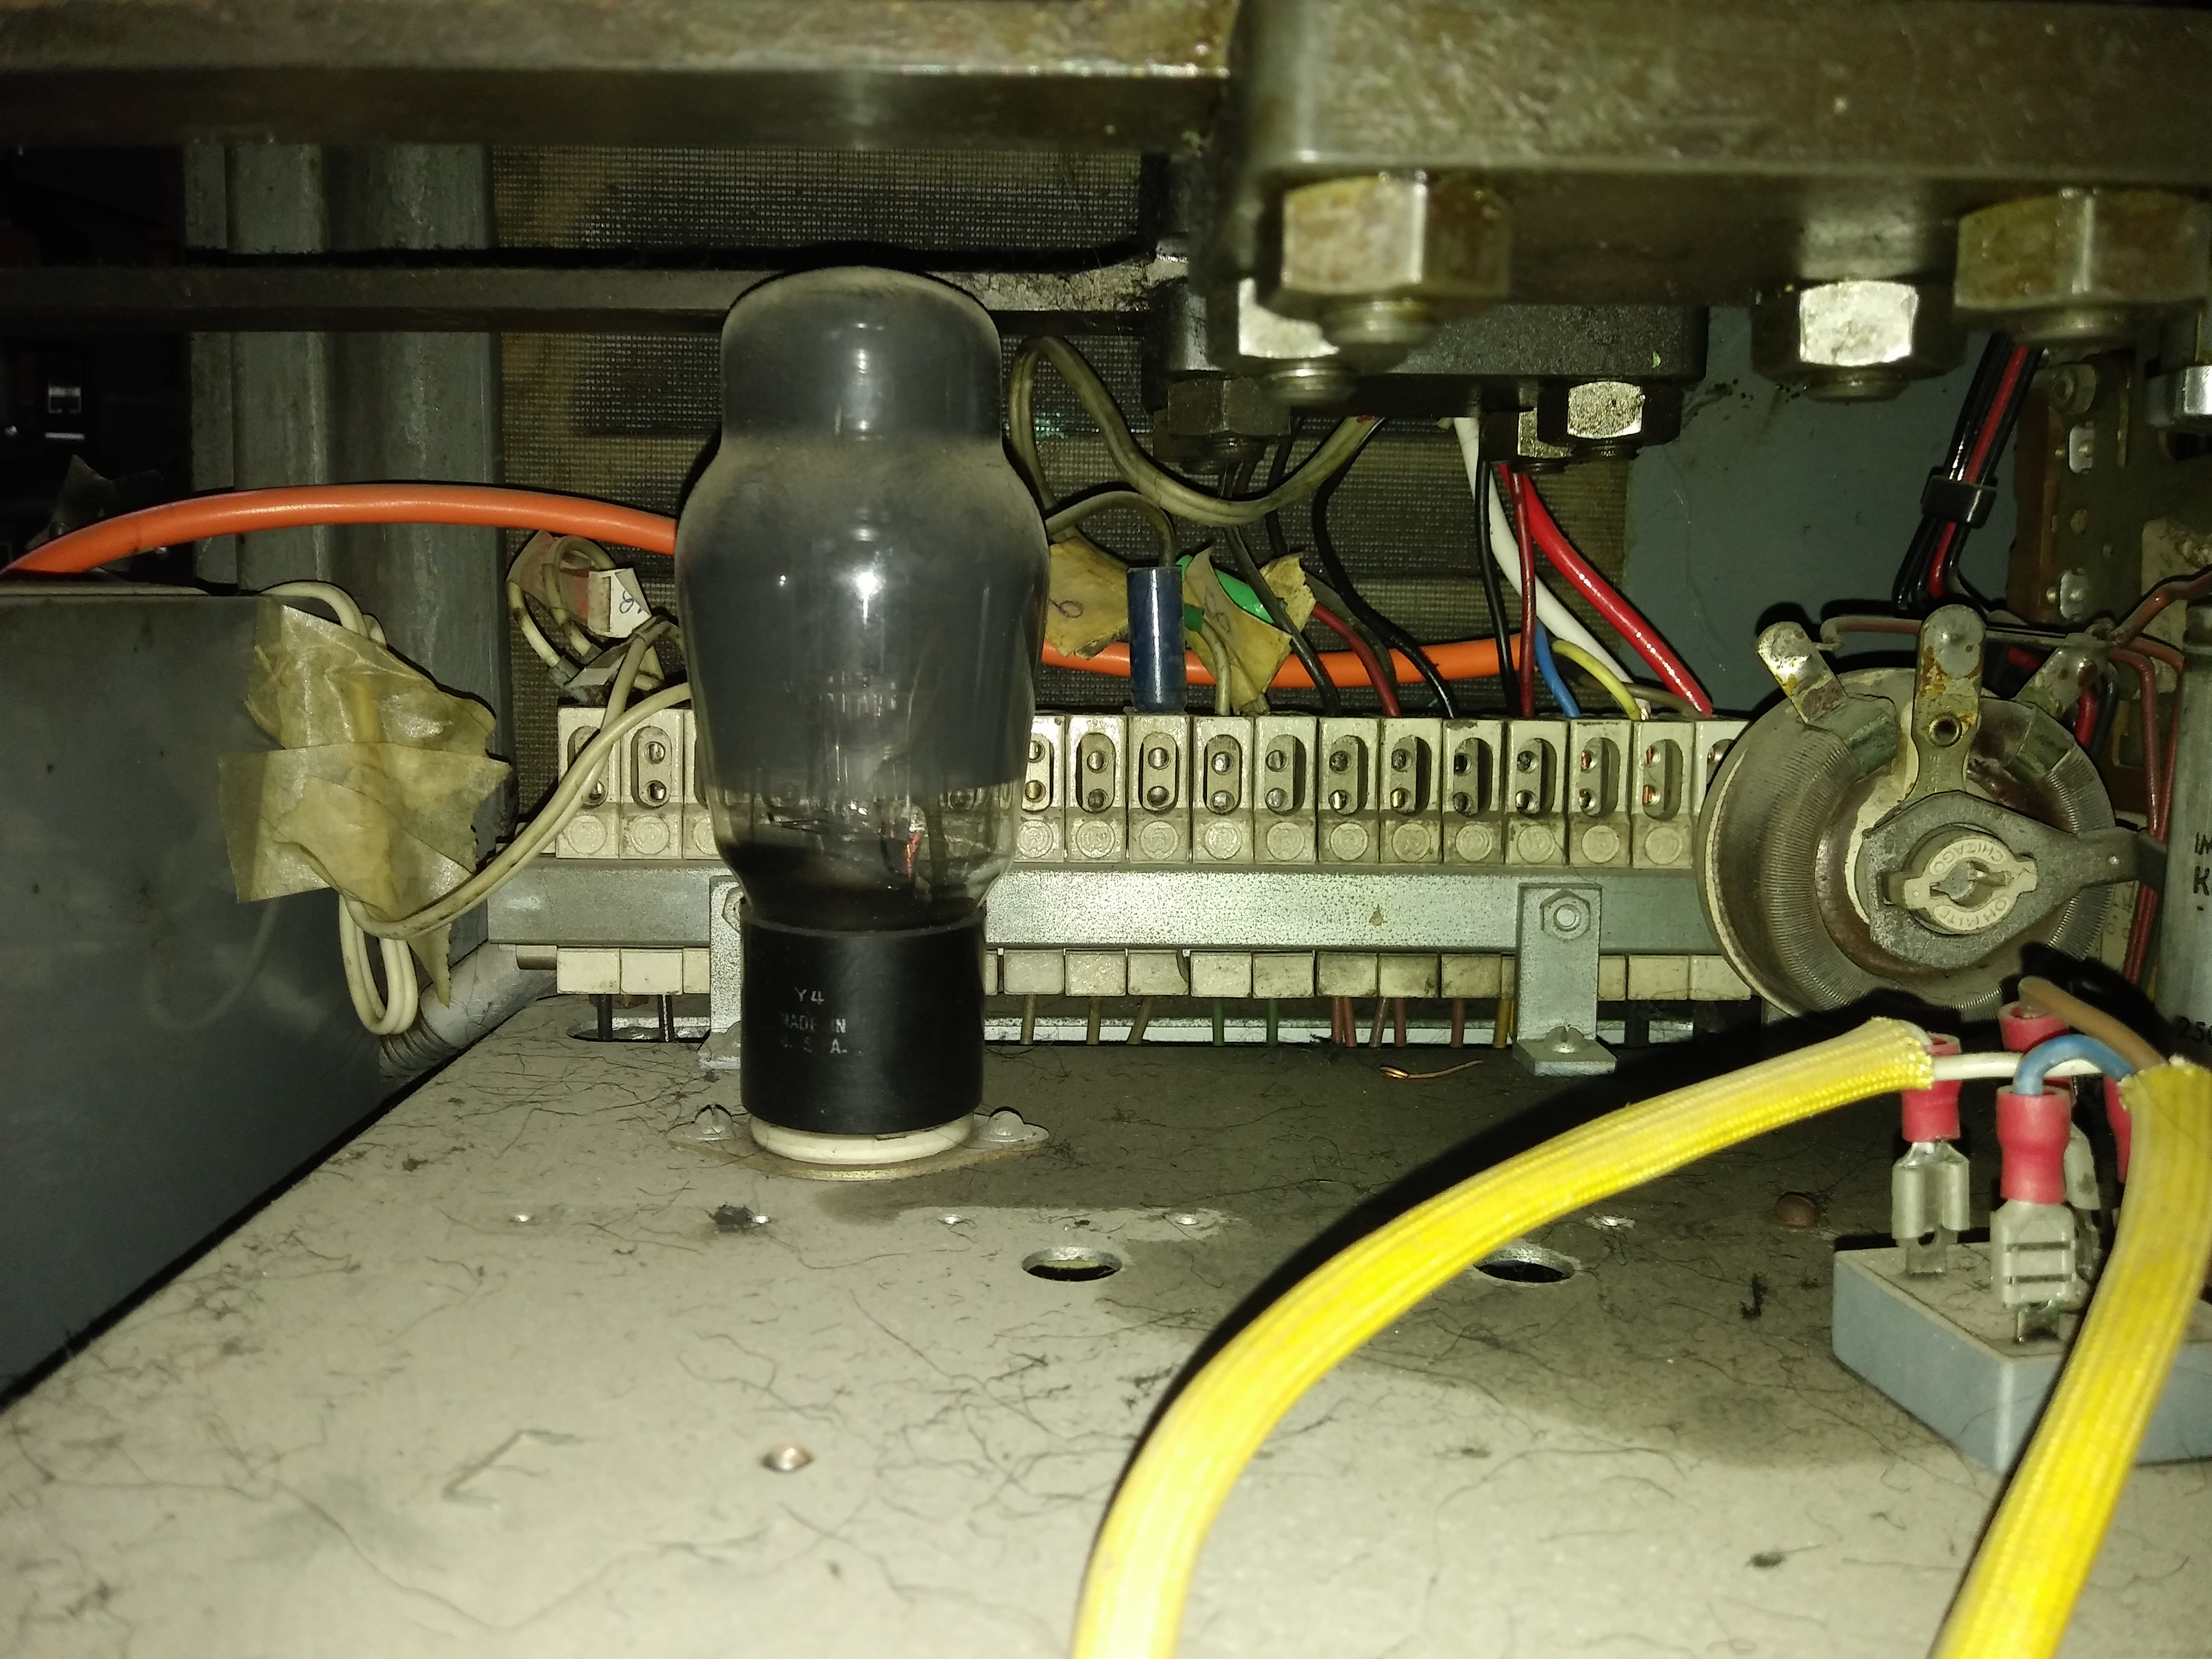
\includegraphics[width=0.98\linewidth]{Imagenes/sist_elec1.jpg}
		\caption{}\label{fig:sist_elect1}
	\end{subfigure}%
	\begin{subfigure}{0.5\linewidth}
		\centering
		\includegraphics[width=0.98\linewidth]{Imagenes/sist_elec2.jpg}
		\caption{}\label{fig:sist_elect2}
	\end{subfigure}%
\caption{En las imágenes (a) y (b) se pueden ver los elementos que componen el sistema eléctrico de la máquina de fatiga.}
\label{fig:sist_elec}
\end{figure}
 
\section{Diseño de estructura}
El proceso de diseñar la estructura hasta su resultado final pasó por distintas etapas. Esto por el proceso de aprendizaje y comprensión de la norma de calculo de madera NCh 1198, como también por la restricción y disponibilidad de materiales, tecnología o medidas acorde a las necesidades. El diseño presentado en este trabajo se muestra en la fig. \ref{fig:mesa_persp}, hecho principalmente de madera, junto a elementos de acero. El objetivo de esta estructura es fijar y soportar la máquina de fatiga tanto en reposo como en operación, buscando como características su durabilidad, lo modular de las piezas y la opción de modificarla en el futuro.

\begin{figure}[h]
\centering
\includegraphics[width=0.9\linewidth, trim={5cm 3cm 5cm 3cm},clip]{Imagenes/mesa_persp.pdf}
\caption{Diseño en perspectiva de la estructura de soporte.}
\label{fig:mesa_persp}
\end{figure}

La metodología de su diseño, se separará en las distintas etapas que se realizó y los requerimientos que surgieron a partir de estas. Finalmente, se realizó una simulación estática y modal para comparar los cálculos realizados y conocer su frecuencia natural, respectivamente.
\subsection{Diseño de pletinas de acero}
La estructura se diseño para que la conexión con la máquina de fatiga fuera a través de pletinas de acero, utilizando los pernos existentes. Las pletinas, a su vez , están conectadas mediante pernos a las vigas principales de madera de cada extremo. Para llevar acabo los cálculo, se hará como suposición que cada pletina esta con un empotramiento en cada extremo, con dos cargas distribuidas. La primera de ellas es el apoyo de la maquina sobre la pletina y, la segunda, el peso propio del acero. Por lo tanto, la fig. \ref{fig:diagcargas_viga_acero} muestra el diagrama de las cargas que actúan y las distancias a utilizar. 

\begin{figure}[h]
\centering
\includegraphics[width=1\linewidth,trim={2cm 1cm 4cm 5cm},clip]{Imagenes/dia_viga_acero.pdf}
\caption{Diagrama de las cargas soportadas por la pletina de acero.}
\label{fig:diagcargas_viga_acero}
\end{figure}

Por otro lado, al no conocerse la distribución de masa de la maquina de fatiga, se considerará la carga distribuida en cada pletina como:
\begin{equation}
	 q_{maq} = \frac{0,75\cdot m_{maq}}{c} = 384,62 \; [\text{kg/m}]
\end{equation}
Donde $m_{maq}$ es la masa estimada en la ec. \ref{eq:masa_maq}, multiplicada por 0,75 como factor de seguridad por la distribución irregular de peso de la máquina. Para obtener el esfuerzo máximo flector es necesario conocer la geometría de la viga, motivo por la cual se iteró entre las distintas opciones disponibles en el mercado de pletinas o barras planas de acero. Por razones estipuladas en la norma NCh 1198, la conexión entre la pletina de acero y la viga principal de madera se debe realizar con un mínimo de dos pernos, por lo tanto, se escogió el ancho máximo del mercado. Así, la tabla \ref{tab:dimycar_pletina} muestra las dimensiones de la pletina escogida.
\begin{table}[h]
\centering
\begin{tabular}{@{}ll@{}}
\toprule
Características pletina			       			& Valor        \\ \midrule
Espesor ($h_p$) {[}mm{]}              			& 8            \\
Ancho ($b_p$) {[}mm{]}               		    & 100          \\
Material    		                		    & A270ES	   \\
Carga distribuida ($q_{ac}$) {[}kg/m{]}		    & 6,28         \\ \bottomrule
\end{tabular}
\caption{Dimensiones y características de la viga de acero}
\label{tab:dimycar_pletina}
\end{table}

Por ende, el cálculo de la reacción en sus apoyos, el momento y esfuerzo flector máximo queda expresado por las ecuaciones \ref{eq:reaccion_acero}, \ref{eq:mtofleca_acero} y \ref{eq:esfmax_acero}, respectivamente. Estas fueron calculadas respecto al punto $A$ (o $B$, por simetría), donde se encuentra el momento flector máximo.

\begin{subequations}
	\begin{gather}
		R_A = g\left(\frac{m_{maq}}{2} + \frac{q_{ac}L}{2}\right) \label{eq:reaccion_acero}\\ 
		M_A = \left(\frac{gcq_{maq}}{24L}\right) \left(3L^2 - 4c^2 + \frac{6bc^2}{L} - \frac{3c^3}{L}\right) + \left(\frac{gq_{ac}L^2}{12}\right) \label{eq:mtofleca_acero} \\
		\sigma_{max,pl} = \frac{M_A \cdot h_p}{2\bar{I}_{pl}} \label{eq:esfmax_acero}
	\end{gather}
\end{subequations}

Así, los valores obtenidos son:
\begin{itemize*}
	\item $R_A = 754,85$ [N]
	\item $M_A = 100,97$ [Nm]
	\item $\bar{I}_{pl} = 4266,6$ [mm$^4$]
	\item $\sigma_{max} = 94,66$ [MPa]
\end{itemize*}

Con relación a la cargas fluctuantes que recibirán las pletinas como parte del funcionamiento de la máquina, se considerará la carga mayor que es capaz de producir la máquina de todas sus configuraciones, de acuerdo a lo que se obtenga por medio del modelo que se expondrá en la sección \ref{sec:mod_sist}. Esta carga alternante sobre la pletina, $F_{a,pl}$, se considerará igual a la mitad de la carga máxima posible producida por el disco desbalanceado. Por lo tanto, considerando la configuración utilizada en las cargas estáticas, la carga distribuida alternante será $q_{a,pl} = F_{a,pl}/c$ y el momento flector máximo en el punto $A$ es la primera expresión de la ec. \ref{eq:mtofleca_acero} y el esfuerzo sobre el mismo punto igual a la expresión \ref{eq:esfmax_acero}, quedando: 
\begin{gather}
	M_{a,pl,A} = \left(\frac{cq_{a,pl}}{24L}\right) \left(3L^2 - 4c^2 + \frac{6bc^2}{L} - \frac{3c^3}{L}\right) \label{eq:mtofat_pletacero}\\
	\sigma_{a,A} = \frac{M_{a,pl,A} \cdot h_p}{2\bar{I}_{pl}} \label{eq:esffat_pletacero}
\end{gather}

Para obtener el factor de seguridad, se utilizará la ecuación de Goodman modificada (ec. \ref{eq:good_mod}). Para esto, el límite de resistencia a la fatiga de un acero se puede estimar como $S_e = 0,5S_{u}$ cuando el esfuerzo último es menor a 1400 MPa \cite{budynas2008shigley}. Como el material utilizado es un acero A270ES, entonces su equivalente en la antigua nomenclatura chilena de acero es A42-27ES \cite{nch203}, donde el esfuerzo último del material es $S_{u} = 420$ MPa, por lo tanto, $S_e = 210$ MPa. También, el esfuerzo medio será igual al esfuerzo estático calculado anteriormente, donde, $S_m = \sigma_{max,pl}$. Así, el factor de seguridad es:
\begin{equation}\label{eq:fs_fatacero}
	\text{FS} = \left(\frac{S_e\cdot S_{ut}}{S_a\cdot S_{ut} + S_m\cdot S_e}\right)
\end{equation}


\subsection{Diseño en madera}
La elección de la madera como elemento principal de construcción se debió por su capacidad de disipar las vibraciones y la relación entre su resistencia y el peso, volviendo la estructura más liviana y útil para las necesidades. Para realizar los cálculos de la madera y sus uniones, se utilizó la norma NCh 1198 Of. 91 \cite{nch1198}, sintetizada en el anexo \ref{ch:anexo_a} para los requerimientos de este trabajo. Las dimensiones del diseño de la estructura se realizaron considerando dejar el espacio necesario para la operación de la máquina, conservando la altura actual de 900 [mm]. Si bien en el presente trabajo se expondrán los cálculos de una especia maderera y sus respectivas dimensiones, se realizaron cálculos con otras especies y en otros formatos para probar distintas configuraciones antes de llegar al diseño propuesto. Las maderas consideradas fueron el pino Oregón, pino Radiata y la línea de pino radiata encolado Hilam de Arauco. Los resultados mostrados en la sección siguiente son los obtenidos al escoger el pino Oregón en formato de 110x110 [mm]. Los valores de las tensiones admisibles para distintas especies madereras se obtienen de la tabla 4 de la sección 6.2 de la NCh 1198, sin embargo, para la madera laminada encolada se encuentran en la norma NCh 2165. Finalmente, para la sección de diseño en madera se utilizará la nomenclatura utilizada por la norma NCh 1198, para evitar confusiones al momento de consultar el anexo o la norma misma.

\subsection{Cálculo de cargas en estructura de madera}
Para identificar las distintas partes de madera en la estructura, se utilizará la fig. \ref{fig:mesa_iso} como referencia. Tanto las vigas A, C, D y el pilar B, están diseñados en base a la misma especie maderera y las vigas A, C y el pilar B del mismo formato. En el anexo \ref{sec:planos} se pueden apreciar los planos del diseño de la estructura propuesta y sus uniones.

\begin{figure}[h]
\centering
\includegraphics[width=1\linewidth, trim={10cm 5cm 7cm 3cm},clip]{Imagenes/mesa_iso.png}
\caption{Identificación de las distintas partes de madera de la estructura soportante.}
\label{fig:mesa_iso}
\end{figure}

Como se nombró anteriormente, la madera utilizada será pino oregón, el cual bajo las consideraciones de la tabla \ref{tab:tabla3_1198} se trabajará como madera seca tanto en construcción como en servicio al estar en un ambiente cerrado sin calefacción, como se señala en la sección de contenido de humedad, \ref{sec:contenido_humedad}. Los valores de densidad, tanto anhidra como normal, se pueden obtener del anexo E de la norma. A partir de este anexo, la tabla \ref{tab:densidad_oregon} muestra los valores admisibles del pino oregón.

\begin{table}[h]
\centering
\resizebox{\textwidth}{!}{%
\begin{tabular}{@{}ccccc@{}}
\toprule
\multirow{2}{*}{\begin{tabular}[c]{@{}c@{}}Especie \\ maderera\end{tabular}} & \multicolumn{2}{c}{Densidad anhidra (kg/m$^3$)}                                                                                                & \multicolumn{2}{c}{Densidad normal (kg/m$^3$)}                                                                                                     \\ \cmidrule(l){2-5} 
                                                                             & \begin{tabular}[c]{@{}c@{}}Valor medio \\ $\rho_o$\end{tabular} & \begin{tabular}[c]{@{}c@{}}Valor característico\\ $\rho_{o,k}\,^{\dagger}$\end{tabular} & \begin{tabular}[c]{@{}c@{}}Valor medio \\ $\rho_{12}$\end{tabular} & \begin{tabular}[c]{@{}c@{}}Valor característico\\ $\rho_{12,k}\,^{\dagger}$\end{tabular} \\ \midrule
Pino oregón                                                                  & 410                                                             & 326                                                                          & 441                                                                 & 350                                                                          \\ \bottomrule
\end{tabular}%
}
\caption{Valores de la densidad normal y anhidra del pino oregón. $^{\dagger}$: Definido con el percentil 5\% de exclusión. \cite{nch1198}}
\label{tab:densidad_oregon}
\end{table}

\subparagraph{Tensiones admisibles y módulo de elasticidad del pino oregón.}
Para la determinación de estos valores es necesario catalogar el grado de calidad, si corresponde a madera verde o seca y la clasificación de la madera del pino oregón. El agrupamiento de las maderas crecidas en Chile se encuentran en el anexo A de la norma NCh 1198, según la cual el pino oregón se clasifica en el grupo ES 5 para madera seca y se asumirá un grado estructural N$^{\circ}$ 4. Con esta información, a través de la tabla 6 de la norma, obtenemos que la clase estructural es F8. Con esto, la tabla 4 y 5 entrega la información de las tensiones admisibles y el módulo de elasticidad. Así, la tabla \ref{tab:tadm_oregon} muestra los valores del pino oregón utilizado en este trabajo.

\begin{table}[h]
\centering
\resizebox{\textwidth}{!}{%
\begin{tabular}{@{}ccccccc@{}}
\toprule
\begin{tabular}[c]{@{}c@{}}Clase\\ Estructural\end{tabular} & \begin{tabular}[c]{@{}c@{}}Flexión\\ $F_f$\end{tabular} & \begin{tabular}[c]{@{}c@{}}Compresión\\ Paralela $F_{cp}$\end{tabular} & \begin{tabular}[c]{@{}c@{}}Compresión\\ Normal $F_{cn}$\end{tabular} & \begin{tabular}[c]{@{}c@{}}Tracción \\ Paralela $F_{tp}$\end{tabular} & \begin{tabular}[c]{@{}c@{}}Cizalle\\ $F_{cz}$\end{tabular} & \begin{tabular}[c]{@{}c@{}}Módulo de\\ elasticidad en\\ flexión $E_f$\end{tabular} \\ \midrule
F8                                                          & 8,6 (MPa)                                               & 6,6 (MPa)                                                              & 4,1 (MPa)                                                            & 5,2 (MPa)                                                             & 0,86 (MPa)                                                 & 6,9 (GPa)                                                                          \\ \bottomrule
\end{tabular}%
}
\caption{Tensiones admisibles y módulo de elasticidad en flexión para madera de pino oregón según su clase estructural. \cite{nch1198}}
\label{tab:tadm_oregon}
\end{table}

\subparagraph{Factores de modificación.}
Dada las condiciones en las que trabajará la madera, se deben calcular dos factores de modificación que afectan de manera global a la madera. La modificación por contenido de humedad se calcula con un factor $\Delta R$ y por la diferencia entre la humedad de la madera y una humedad del 12\%, $\Delta H$. Considerando una humedad de la madera del 15\%, entonces los valores de $K_H$ para cada solicitación se muestran en la tabla \ref{tab:kh_oregon}.
\begin{table}[h]
\centering
\resizebox{\textwidth}{!}{%
\begin{tabular}{ccccccc}
\hline
\begin{tabular}[c]{@{}c@{}}Factor de \\ modificación\\ por humedad\end{tabular} & \begin{tabular}[c]{@{}c@{}}Flexión\\ $F_f$\end{tabular} & \begin{tabular}[c]{@{}c@{}}Compresión\\ Paralela $F_{cp}$\end{tabular} & \begin{tabular}[c]{@{}c@{}}Compresión\\ Normal $F_{cn}$\end{tabular} & \begin{tabular}[c]{@{}c@{}}Tracción \\ Paralela $F_{tp}$\end{tabular} & \begin{tabular}[c]{@{}c@{}}Cizalle\\ $F_{cz}$\end{tabular} & \begin{tabular}[c]{@{}c@{}}Módulo de\\ elasticidad en\\ flexión $E_f$\end{tabular} \\ \hline
$K_H$                                                                           & 0,999385                                                & 0,999385                                                               & 0,999385                                                             & 0,99952                                                               & 0,999199                                                   & 0,999556                                                                           \\ \hline
\end{tabular}%
}
\caption{Valores del factor de modificación para el pino oregón.}
\label{tab:kh_oregon}
\end{table}

Por otro lado, el factor de modificación por duración, $K_D$, se aplica a través de la ec. \ref{eq:k_d}, donde la duración de la carga $t$ se aplica en segundos. También, la norma incluye el gráfico de $K_D$ siendo una opción para su cálculo. Los valores admisibles que se señalan en la norma corresponden a una vida útil de 10 años de duración, sin embargo, para una vida útil indefinida el valor de $K_D$ corresponde a 0,9. Este factor de modificación no afecta al módulo de elasticidad ni a la tensión admisible de compresión normal.
\begin{equation} \label{eq:k_d}
	K_D = \frac{1,747}{t^{0,0464}} + 0,295
\end{equation}

\subsubsection{Viga principal, A}
Es la viga que soporta la carga de las pletinas que sostienen a la máquina y a su vez descansa la carga en los pilares B. Para realizar los cálculos de esfuerzo se consideró un doble empotramiento en cada extremo, con tres cargas distribuidas que representan la carga de las pletinas de acero, $q_{pl}$, las cuales se determinarán según la ec. \ref{eq:q_pl}, y el peso propio de la madera.
\begin{equation}\label{eq:q_pl}
	q_{pl} = \frac{q_{maq}\,c + q_{ac}\,L}{2b_p}
\end{equation}
El diagrama y la distribución de la carga se puede apreciar en la fig. \ref{fig:diagcargas_viga_a}. Por otro lado, el esfuerzo máximo se presenta en los extremos de la viga. Las ecuaciones \ref{eq:reac_vigappal} y \ref{eq:mto_vigappal}, muestran la obtención de las reacciones y del momento flector máximo.
\begin{subequations}
\begin{gather}
	R_0 = g \left( q_{pl}\cdot b_p + \frac{L\cdot q_{mad}}{2}\right) \label{eq:reac_vigappal}\\
	M_0 = \left(\frac{q_{pl}\cdot g\cdot b_p}{L^2}\right) \left(l_2 l_6^2 + l_6 l_2^2 - \frac{b_p^2}{12}\left( l_6 + l_2\right) \right) + \frac{R_0\cdot L}{6} \label{eq:mto_vigappal} 
\end{gather}
\end{subequations}
Donde los valores obtenidos son:
\begin{itemize*}
	\item $R_0 = Q = 795$ [N]
	\item $M_0 = M_{max} = 122,26$ [Nm]
\end{itemize*}
Así, la tensión de trabajo $f_f$ se calcula según la ec. \ref{eq:f_f}, obteniendose el valor:
\begin{equation}
	f_f = 0,551 \quad \text{(MPa)}
\end{equation}
De este modo, la tensión de diseño en la zona flexo-traccionada y flexo-comprimida que se calcula a partir de las ecuaciones \ref{eq:ft_dis} y \ref{eq:fv_dis}, respectivamente. Para la zona flexo-traccionada se debe calcular el factor de modificación por altura y para la flexo-traccionada el factor de modificación por volcamiento. El primero se obtiene con la ec. \ref{eq:khf}, obteniendose el valor de $K_{hf} = 0,916$. Para el factor de volcamiento, se deben verificar el caso que corresponde como se señala en el anexo \ref{ch:anexo_a}, el cual da un valor de $K_v=1$. Por lo tanto, el valor de $F_{ft,dis}$ y $F_{fv,dis}$ son:
\begin{subequations}
\begin{gather}
	F_{ft,dis} = 7,08 \quad \text{(MPa)}\\
	F_{fv,dis} = 7,74 \quad \text{(MPa)} 
\end{gather}
\end{subequations}
Por otro lado, la tensión de trabajo en cizalle se obtiene a partir de la ec. \ref{eq:f_cz} y la de diseño en cizalle por \ref{eq:cz_dis}. Dado que $K_r=1$ al no haber rebaje de la viga, entonces el valor obtenido para ambas tensiones son:
\begin{align}
	f_{cz} &= 0,098 \quad \text{(MPa)}\\
	F_{cz,dis} &= 0,774 \quad \text{(MPa)}
\end{align}

%--------------------------------------------------------
%Finalmente, los valores de factor de seguridad (FS) para cada uno de las tensiones calculadas son los siguientes:
%\begin{subequations}
%\begin{gather}
%	FS_{ft} = 12,85\\
%	FS_{fv} = 14,03\\
%	FS_{cz} = 7,85
%\end{gather}
%\end{subequations}
%--------------------------------------------------------

\begin{figure}[h]
\centering
\includegraphics[width=0.95\linewidth,trim={9cm 3cm 5.3cm 3.5cm},clip]{Imagenes/dia_viga_a.pdf}
\caption{Diagrama de las cargas soportadas por la viga A.}
\label{fig:diagcargas_viga_a}
\end{figure}

\subsubsection{Pilar de apoyo, B}
El pilar B representa los cuatro apoyos de la estructura, recibiendo la carga de la máquina y su operación desde la viga principal y transmitiendola hasta el piso. Por la disposición del cuartón, estará sometido a compresión paralela (sección \ref{sec:cp}). Al igual que en la viga principal, se debe calcular la tensión de trabajo ($f_{cp}$) y la tensión de diseño en compresión paralela ($F_{cp,dis}$). Al ser el mismo formato y especie maderera de la viga principal, su área transversal se mantiene, mientras que el largo del pilar ($L_v$) corresponde a 790 mm.

Para el primero, se obtiene a través de la ecuación \ref{eq:f_cp}, donde la carga $N$ será igual a la reacción obtenida en la ec. \ref{eq:reac_vigappal}. Así, su valor es:


\begin{equation}
	f_{cp} = 0,0657 \quad \text{(MPa)} 
\end{equation}
El valor de $f_{cp}$ será posteriormente corregido una vez que se seleccionen las dimensiones de las uniones mecánicas, recalculando la tensión de trabajo con el área neta.

Para el segundo, el cálculo de la tensión de diseño dependerá de la inestabilidad lateral dado por la esbeltez $\lambda$. La longitud efectiva de pandeo se obtiene a través de la tabla 18 de la norma, de la cual se escogerá la configuración de apoyo con impedimento de giros y desplazamiento por un extremo y, para el otro lado, impedimento de giro con libertad de desplazamiento, es decir, $l_p/L_v = 1,5$. De esta forma, los valores obtenidos son:
\begin{gather*}
	l_p = 1,5\cdot L_v = 1,185 \: \text{(m)}\\
	i = \sqrt{\frac{\bar{I}}{A}} = \sqrt{\frac{0,11^4}{12\cdot 0,11^2}} = 0,032 \: \text{(m)}\\
	\lambda = \frac{l_p}{i} = 37,32 \: \text{(-)}
\end{gather*}
Como $\lambda > 5$, entonces la tensión de trabajo de compresión paralela se debe calcular según la ec. \ref{eq:cp_dislambda} y se debe evaluar el factor de modificación por esbeltez $K_{\lambda}$ a partir de la ec. \ref{eq:k_lambda}. El coeficiente de proporcionalidad para una madera de grado n$^{\circ}$ 4 es $c = 0,8$ y el módulo de elástico de diseño es $E_{dis} = 6206,2\: \text{(MPa)}$. Por otro lado, la tensión de diseño $F_{cp,dis}$ se obtiene a partir de los factores de modificación $K_D$ y $K_H$ y la ecuación \ref{eq:cp_dis}.
\begin{equation}
	F_{cp,dis} = 5,936 \quad \text{(MPa)}
\end{equation}
Con esto, los valores de las constantes serán $A = 2,852$ (-), $B = 3,754$ (-) y el factor de modificación por esbeltez $K_{\lambda} = 0,759$ (-). La tensión de diseño en compresión paralela considerando inestabilidad lateral $F_{cp,\lambda, dis}$ será:
\begin{equation}
	F_{cp,\lambda, dis} = 4,506 \quad \text{(MPa)}
\end{equation}

\subsubsection{Viga transversal, C}
Para esta viga se realizará el mismo procedimiento que para la viga A, sin embargo, las solicitaciones son menores y la única carga a la que está sometida es la de su propio peso. Las dimensiones nominales de la tabla son 1x8'' cepillada, es decir, según las tablas \ref{tab:anchodim} y \ref{tab:espdim} son de 19x185 mm y su largo es de 800 milímetro. La carga distribuida de su peso es de $q_{tabla}=1,5$ [kg/m].

Debido a lo bajo de las solicitudes, las tensiones de trabajo en flexión son:
\begin{equation}
	f_f = 3,804 \: \text{(kPa)} 
\end{equation}
Por otro lado, por las dimensiones de la madera usada, el factor de modificación por altura y volcamiento son los siguientes:
\begin{gather*}
	K_{hf} = 0,864\: \text{(-)}\\
	K_{v} = 0,586\: \text{(-)}
\end{gather*}
El cálculo de $K_v$ se realiza con la ecuación \ref{eq:k_v}, porque la esbeltez del límite elástico es menor a la esbeltez de volcamiento.
\begin{gather*}
	\lambda_v = 23,38 \: \text{(-)}\\
	\lambda_{vo} = 21,95 \: \text{(-)}
\end{gather*}
Así, la tensión de diseño en flexión de esta viga es de:
\begin{equation}
	F_f = 3,9235 \: \text{(MPa)}
\end{equation}

\subsection{Uniones}
Las uniones en madera se deben diseñar siguiendo las indicaciones establecidas en la sección 10 de la norma NCh1198, uniones en la madera estructural. Esta considera la condición de la madera en operación, el tipo de unión, la dirección de la solicitación respecto a la dirección de la fibra, el número de elementos de unión, el distanciamiento entre los elementos de unión y el tipo de cizalle. Para el diseño de la estructura se utilizaron tres elementos de unión distintos: tirafondos, pernos y, en menor medida, clavos.

\subsubsection{Acero - madera}
Para la unión entre la pletina de acero y la viga principal de madera, se utilizaron dos pernos de grado 2 de 5 \nicefrac{1}{2}'' de largo y  $1/4''$ de diámetro. Como se explica en la sección \ref{sec:union_perno}, el mínimo de pernos por unión debe ser dos, con la excepción de que el único perno no esté solicitado en un porcentaje superior al 50\% de su capacidad de diseño. La unión está compuesta por la pletina de acero, seguido por la viga de madera con la dirección de sus fibras normal a las solicitaciones y nuevamente una placa de acero. Finalmente, para el cálculo de la capacidad de carga admisible y tensión admisible de aplastamiento nominal, se recurrirá a las ecuaciones \ref{eq:padm_ad} y \ref{eq:f_ap}, respectivamente. 

Para calcular la capacidad de carga admisible, $P_{ad}$, se utilizaron las indicaciones para cizalle simple, las cuales indican que se determina como el menor valor de la mitad de la carga admisible de cizalle doble entre una pieza central de espesor igual a la pieza más grande y una pieza central igual al doble del espesor de la pieza más delgada. Para este diseño el valor menor consiste en considerar el espesor central ficticio $e*$ como dos veces el espesor menor, es decir, el espesor lateral $e_l$, así el valor de esbeltez del perno es:  
\begin{equation*}
	\lambda_u = \frac{2\cdot e*}{D} = \frac{2\cdot 8\, \text{mm}}{9,525\, \text{mm}} = 1,679\: \text{(-)}
\end{equation*}
Para obtener $F_{ap}$ se utiliza la ecuación \ref{eq:f_ap}. El valor del factor de reducción de zona elástica se obtiene a partir de la densidad anhidra de la madera (tabla \ref{tab:densidad_oregon}), siendo $\eta =$ 2,2. Por otro lado el ángulo $\theta$ es de $\pi/2$ al estar las fuerzas en dirección normal a la fibra de madera. Con esto, se obtiene:
\begin{gather}
	F_{ap} = 3,402 \: \text{(MPa)} \\
	P_{ad,simple} =\frac{P_{ad,doble}}{2} = 259,24 \: \text{(MPa)}
\end{gather}
Para terminar, se debe corroborar que se cumple la desigualdad de la ecuación \ref{eq:padm_ad}, así:
\begin{equation*}
	Z\cdot D^2 = 2131,94 \: \text{(MPa)} \geq 259,24 \: \text{(MPa)}
\end{equation*}

\subparagraph{Espaciamiento}
El espaciamiento entre los pernos se especifica en la sección \ref{sec:espaciamiento_pernos}, de las cuales se obtiene la distancia entre pernos y los bordes es:
\begin{align*}
	S_{bcn} &= 1,5 \, \text{mm} \\
	S_{bdn} &= 0,75 \, \text{mm} \\
	S_p &= 2,625 \, \text{mm}
\end{align*}


\subsubsection{Madera - Madera}
Existen distintos componentes de unión para la conexión de elementos de madera. En este trabajo se utilizó el tirafondo, perno y clavo como elementos principales de unión.  Cada uno de ellos tiene distintas características que los vuelven ventajosos en ciertas situaciones. La utilización del tirafondo se utiliza para unir la viga C con el pilar B y la viga A, por su capacidad de ``empujar'' una madera contra la otra de manera eficiente. Los pernos, por otro lado, se utilizaran para la unión de herrajes entre la viga D y el pilar B, como también en los herrajes de anclaje del pilar B con el piso. En el caso de los clavos, estos se ocupan en los ángulos de apoyo entre las vigas A y B, para evitar su movimiento transversal. Para estos dos últimos elementos de unión, su elección está supeditada a las recomendaciones del fabricante de los herrajes o ángulos, quienes incluyen los valores de carga en la elección de los elementos de unión. Por lo mismo, la caracterización de estos elementos se realizará en la sección de conectores.

\subsubsection{Tirafondos}
Las indicaciones para el cálculo, espaciamiento e instalación de los tirafondos se encuentran en la sección \ref{sec:tirafondos}. Al igual que el proceso de selección de vigas de madera, se iteró con distintas dimensiones de largo y diámetro. De esta manera, el tirafondo escogido fue de $1/4$ x 1\nicefrac{1}{2}'', lo cual se traduce a partir del anexo M de la norma en las medidas expuestas en la tabla \ref{tab:tirafondo}.
\begin{table}[h]
\centering
\resizebox{\textwidth}{!}{%
\begin{tabular}{@{}cccccl@{}}
\toprule
\begin{tabular}[c]{@{}c@{}}Nomenclatura\\ tirafondo\end{tabular} & \begin{tabular}[c]{@{}c@{}}Diámetro Nominal \\ ($D_v$ o $D$) [mm]\end{tabular} & \begin{tabular}[c]{@{}c@{}}Diámetro de rosca\\  ($D_R$) [mm]\end{tabular} & \begin{tabular}[c]{@{}c@{}}Largo roscado\\  (R) [mm]\end{tabular} & \begin{tabular}[c]{@{}c@{}}Largo vástago\\ (V) [mm]\end{tabular} & \begin{tabular}[c]{@{}l@{}}Largo punta\\ (P) [mm]\end{tabular} \\ \midrule
$1/4$ x 3\nicefrac{1}{2}''                                         & 6,4                                                                            & 4,4                                                                       & 51                                                                & 38                                                               & 4,8                                                            \\ \bottomrule
\end{tabular}%
}
\caption{Dimensiones del tirafondo utilizado}
\label{tab:tirafondo}
\end{table}

Para su instalación, la norma indica que es necesario realizar perforaciones guías, las cuales están en función de sus características. Así el agujero tendrá dimensiones para la zona del vástago y otra para la zona con rosca. Para la zona del vástago, el agujero deberá tener las dimensiones del diámetro nominal $D_v$ y el largo V. Para la segunda zona, la madera de pino oregón se categoriza en el grupo B según su densidad anhidra, a partir de la tabla 38 de la norma. Con esta información el largo del agujero debe ser de R - P  y el diámetro del entre el 60\% y el 70\% de $D_v$.
\paragraph{Solicitaciones de extracción lateral}
La carga admisible de extracción lateral se calcula según la ecuación \ref{eq:pel_ad}. El valor K se obtiene a partir de la tabla 39 de la norma dependiendo de si la madera utilizada es conífera o latifoliada y su densidad anhidra. El pino oregón es una madera conífera y, según su densidad, el valor de K es de 11,7. Así el valor obtenido es de $P_{el,ad} = 0,48$ (kN). Sin embargo, la norma establece tres condiciones que se deben cumplir para que la expresión \ref{eq:pel_ad} sea aplicable, de las cuales no se cumple que el espesor $e_L$ de la pieza lateral atravesada por el tirafondo sea igual a $3,5\cdot D$. Por esto se debe mayorar el valor de la carga admisible por factores de modificación que pueden penalizar o ayudar, dependiendo de la configuración de la unión.

\subparagraph{Factor de modificación por espesor de la pieza lateral.}
El factor se obtiene a partir de la tabla 40 de la norma, debido a que $e_L \neq 3,5\cdot D$. El valor $K_{te}=0,93$ se obtiene al ingresar a la tabla con la razón $e_L/D \approx 3$.

\subparagraph{Factor de modificación por penetración del vástago en la pieza principal.}
De manera análoga, el factor se obtiene en la tabla 41 de al norma a partir de la razón entre la penetración del vástago en la pieza, $P_v$, y el diámetro del tirafondo. El valor de este es $P_v/D \approx 5$, lo cual da que $K_v=1,36$

\subparagraph{Factor de modificación por diámetro.}
Por último, este factor se obtiene directamente del diámetro nominal del tirafondo, a través de la tabla 42 de la norma. El valor corresponde a $K_{tD}=0,97$.
\\

Además de los factores de modificación expuestos, el eje del tirafondo se encuentra en dirección paralela a las fibras de la madera de la pieza principal, por lo tanto se debe multiplicar el valor de la carga admisibles por $\frac{2}{3}$. En conclusión, la carga admisible es igual a :
\begin{equation}
	P_{el,ad} = \frac{2}{3}\cdot K_{te}\cdot K_{tv}\cdot K_{tD} \cdot K\cdot D^2\cdot = 391,966 \: \text{(N)}
\end{equation}

\paragraph{Solicitaciones de extracción directa}
Para el caso de la extracción directa es la ecuación \ref{eq:ped_ad} la que determina la carga admisible de tirafondos colocados con su eje normal a las fibras de la madera. Dado que este no es el caso, como se señaló en la sección de extracción lateral, la carga admisible a considerar se debe multiplicar por $\frac{3}{4}$. Por otra parte, el valor de la longitud crítica de penetración $l_{crit}=10\cdot D_R$ se obtuvo de la tabla 43 de la norma. Sin embargo, la longitud real de penetración de la zona roscada (R-P) es menor a la longitud crítica, por lo tanto en la ecuación se reemplaza $l_{crit}$ por $l = R-P$. Entonces el valor obtenido para la carga admisible es:
\begin{equation}
	P_{ed,ad} = 6,37 \: \text{(kN)}
\end{equation} 

\subsubsection{Conectores}
La elección de los conectores utilizados se basó en tres aspectos principales: la disponibilidad de los productos en la región, la compatibilidad con los elementos de madera y con las cargas que pueden resistir según el fabricante. Estos consisten en un elemento de metal, acero generalmente, que permite la unión de dos o más piezas de madera para soportar determinadas cargas. Existen en distintas geometrías y, el mecanismos de conexión entre acero y madera, es a través de elementos de unión mecánica, es decir, pernos, clavos y tornillos, principalmente. Para este trabajo se utilizaron tres tipos, los cuales une las vigas A-B, B-D y B con el suelo del laboratorio, todos fabricados por la marca Simpson Strong-Tie.

Para la unión entre A y B se utilizó en el diseño un ángulo de unión modelo A44, donde la longitud de sus brazos es de 4 \nicefrac{9 }{ 16}'' y 4 \nicefrac{3 }{ 8}'' de largo y su ancho de 1,5 pulgadas. Los elementos de unión a utilizar son clavos de 0,148'' de diámetro y 3'' de largo. Las fuerzas que soportan, de acuerdo a la imagen \ref{fig:a24}, son de $F_1=$ 3,45 kN y $F_2=$ 1,23 kN. 

\begin{figure}[h]
\centering
\includegraphics[width=0.3\linewidth]{Imagenes/a24.pdf}
\caption{Representación de un ángulo de unión A44 y A66. \cite{angleconnector}}
\label{fig:a24}
\end{figure} 

Para la unión del pilar B y la viga D se utilizó el ángulo A66. Este se une a través cada brazo de 5 \nicefrac{7 }{ 8}'' a través de unos pernos de diámetro de \nicefrac{3 }{ 8}''. Estos buscan soportar la carga provocada por el propio peso y evitar los desplazamientos horizontales. Su disposición se puede ver en los planos del anexo \ref{sec:planos}, donde se aprecia cómo se utilizan dos ángulos por conexión.

Por último, la unión entre el piso y el pilar B se escogió un ángulo de anclaje A24. Utiliza un perno de anclaje y uno de sujeción de \nicefrac{1 }{ 2}'' para el piso y otro normal que es adosado en el otro extremo del pilar por un segundo ángulo de anclaje, de manera similar a la unión B-D. El plano del anexo \ref{sec:planos} muestra en detalle el diseño de la conexión.
 
\subsection{Simulaciones}
Las simulaciones de la máquina se utilizaron como apoyo y contraparte de los cálculos realizados manualmente. Éstas se realizaron en el software Inventor AutoCAD, en el ambiente ``\textit{Stress Analysis}''. A través de esto, se busca confirmar que los resultados obtenidos en los cálculos estáticos se encuentran fuera de los rangos de falla y obtener las frecuencias naturales de la estructura, utilizando ``\textit{Static and Modal Analysis}''.

Debido a las limitantes del programa utilizado, se debieron adaptar las propiedades mecánicas ortotrópicas de la madera, las cuales no era posible simular directamente. Para esto, se utilizaron los valores mínimos del Módulo de Young y las tensiones admisibles en las direcciones de mayor solicitación de cada elemento, buscando representar de manera segura las propiedades ortotrópicas en una configuración isotrópica.

Como condición del problema, en ambas simulaciones, las restricciones de los pilares de apoyo B se consideran empotrados (\textit{fixed}), impidiendo cualquier grado de movimiento en su base. Además, las uniones se consideraron perfectas y sin desplazamientos. La carga fue aplicada en forma de presión sobre la parte superior de la máquina de fatiga para tener una distribución adecuada del peso de la misma, tomando en consideración la masa calculada en la ec. \ref{eq:masa_maq} de 200 kg.

\subsubsection{Análisis modal}
La configuración utilizada para realizar esta simulación consistió en\footnotemark . 
\begin{itemize*}
	\item Número de modos: 6
	\item Rango de frecuencias: 0 - 120 Hz
	\item Precisión mejorada (\textit{Enhanced Accuracy)}
	\item Contactos:
		\begin{itemize*}
			\item Tolerancia: 0,1 mm
			\item Tipo: \textit{Bonded}
		\end{itemize*}
	\item Malla:
		\begin{itemize*}
			\item Tamaño medio del elemento: 0,08
			\item Tamaño mínimo del elemento: 0,15
			\item Factor de modificación: 1,5 (default)
			\item Ángulo máximo de giro: 60 grados (default)
			\item Calcular modos precargados
			\item Utilizar la medida para la malla según la pieza base del ensamblaje
		\end{itemize*}
\end{itemize*}

\subsubsection{Análisis estático}
Para realizar la simulación estática se retiraron todos los elementos de unión, es decir, pernos, tirafondos, conectores y ángulos, conservando solo las vigas de madera y las pletinas de acero. El fin de esto es analizar específicamente los esfuerzos a los que están sometidos estos elementos a la carga de la máquina de fatiga. La configuración principal de la simulación consiste en\footnotemark[\value{footnote}]:
\footnotetext{La definición de cada opción se encuentra en el manual de Autodesk Inventor. \cite{autodesk}}
\begin{itemize*}
	\item Detectar y eliminar modos de cuerpo rígido
	\item Separar tensiones en superficies de contacto
\end{itemize*}
La configuración de los contactos y la malla se conservó igual a la establecida en el análisis modal.

\section{Modelo dinámico del sistema}
Luego del levantamiento de información, se busca analizar y predecir el comportamiento de la máquina en sus distintas configuraciones. Para esto se utiliza la información disponible para realizar un modelo del funcionamiento de la máquina de fatiga, en específico, de la carga aplicada a la probeta en función de la velocidad de rotación del disco y las distintas combinaciones de contrapesos. El disco se encuentra en voladizo, cuyo desequilibrio a partir de los contrapesos colocados produce una fuerza que es transmitida hacia un brazo de carga. Este, a su vez, aplica un momento de flexión sobre una probeta que está doblemente empotrada por mordazas.

Para obtener el comportamiento y la fuerza que produce el desbalanceo en el disco sobre la probeta, se modelará un sistema de dos grados de libertad para representar el movimiento de la máquina y sus componentes, realizando ciertas simplificaciones y suposiciones. Se utilizará el método de energía derivar las ecuaciones de movimiento del sistema.

A través de esto, se pretende obtener la posición en reposo de la máquina y la deformación máxima que sufre la probeta según cada configuración. En concreto, la posición en reposo de la máquina, es decir, la deformación producto de la gravedad, entregará información sobre cual es la carga media y esfuerzo medio que sufre la probeta. En cambio, la deformación máxima es la información relativa a la carga alternante que se le aplica a la probeta y su correspondiente esfuerzo alternante. Por ello, el modelo deberá partir de una posición a conveniencia en un tiempo inicial y sin fuerzas externas interviniendo. Posteriormente, una vez que se haya alcanzado la posición de equilibrio, la fuerza externa producida por el disco desbalanceado comenzará a funcionar hasta que vibre de manera estacionaria. Al respecto, al ser la fuerza dependiente de la velocidad angular del disco, se introducirá una función que llamaremos $\phi$ la cual controlará la aceleración y velocidad del disco.

\subsection{Elementos del sistema}
La fig. \ref{fig:elementos_modelo} muestra todas los elementos que participan en el funcionamiento de la máquina y que afectan su comportamiento. Sin embargo, estos se llevarán a un diagrama que representará los elementos y las simplificaciones utilizadas para modelar el movimiento de la máquina, en específico, del brazo de carga.  

\begin{figure}[p]
\centering
	\begin{subfigure}{1\linewidth}
		\centering
		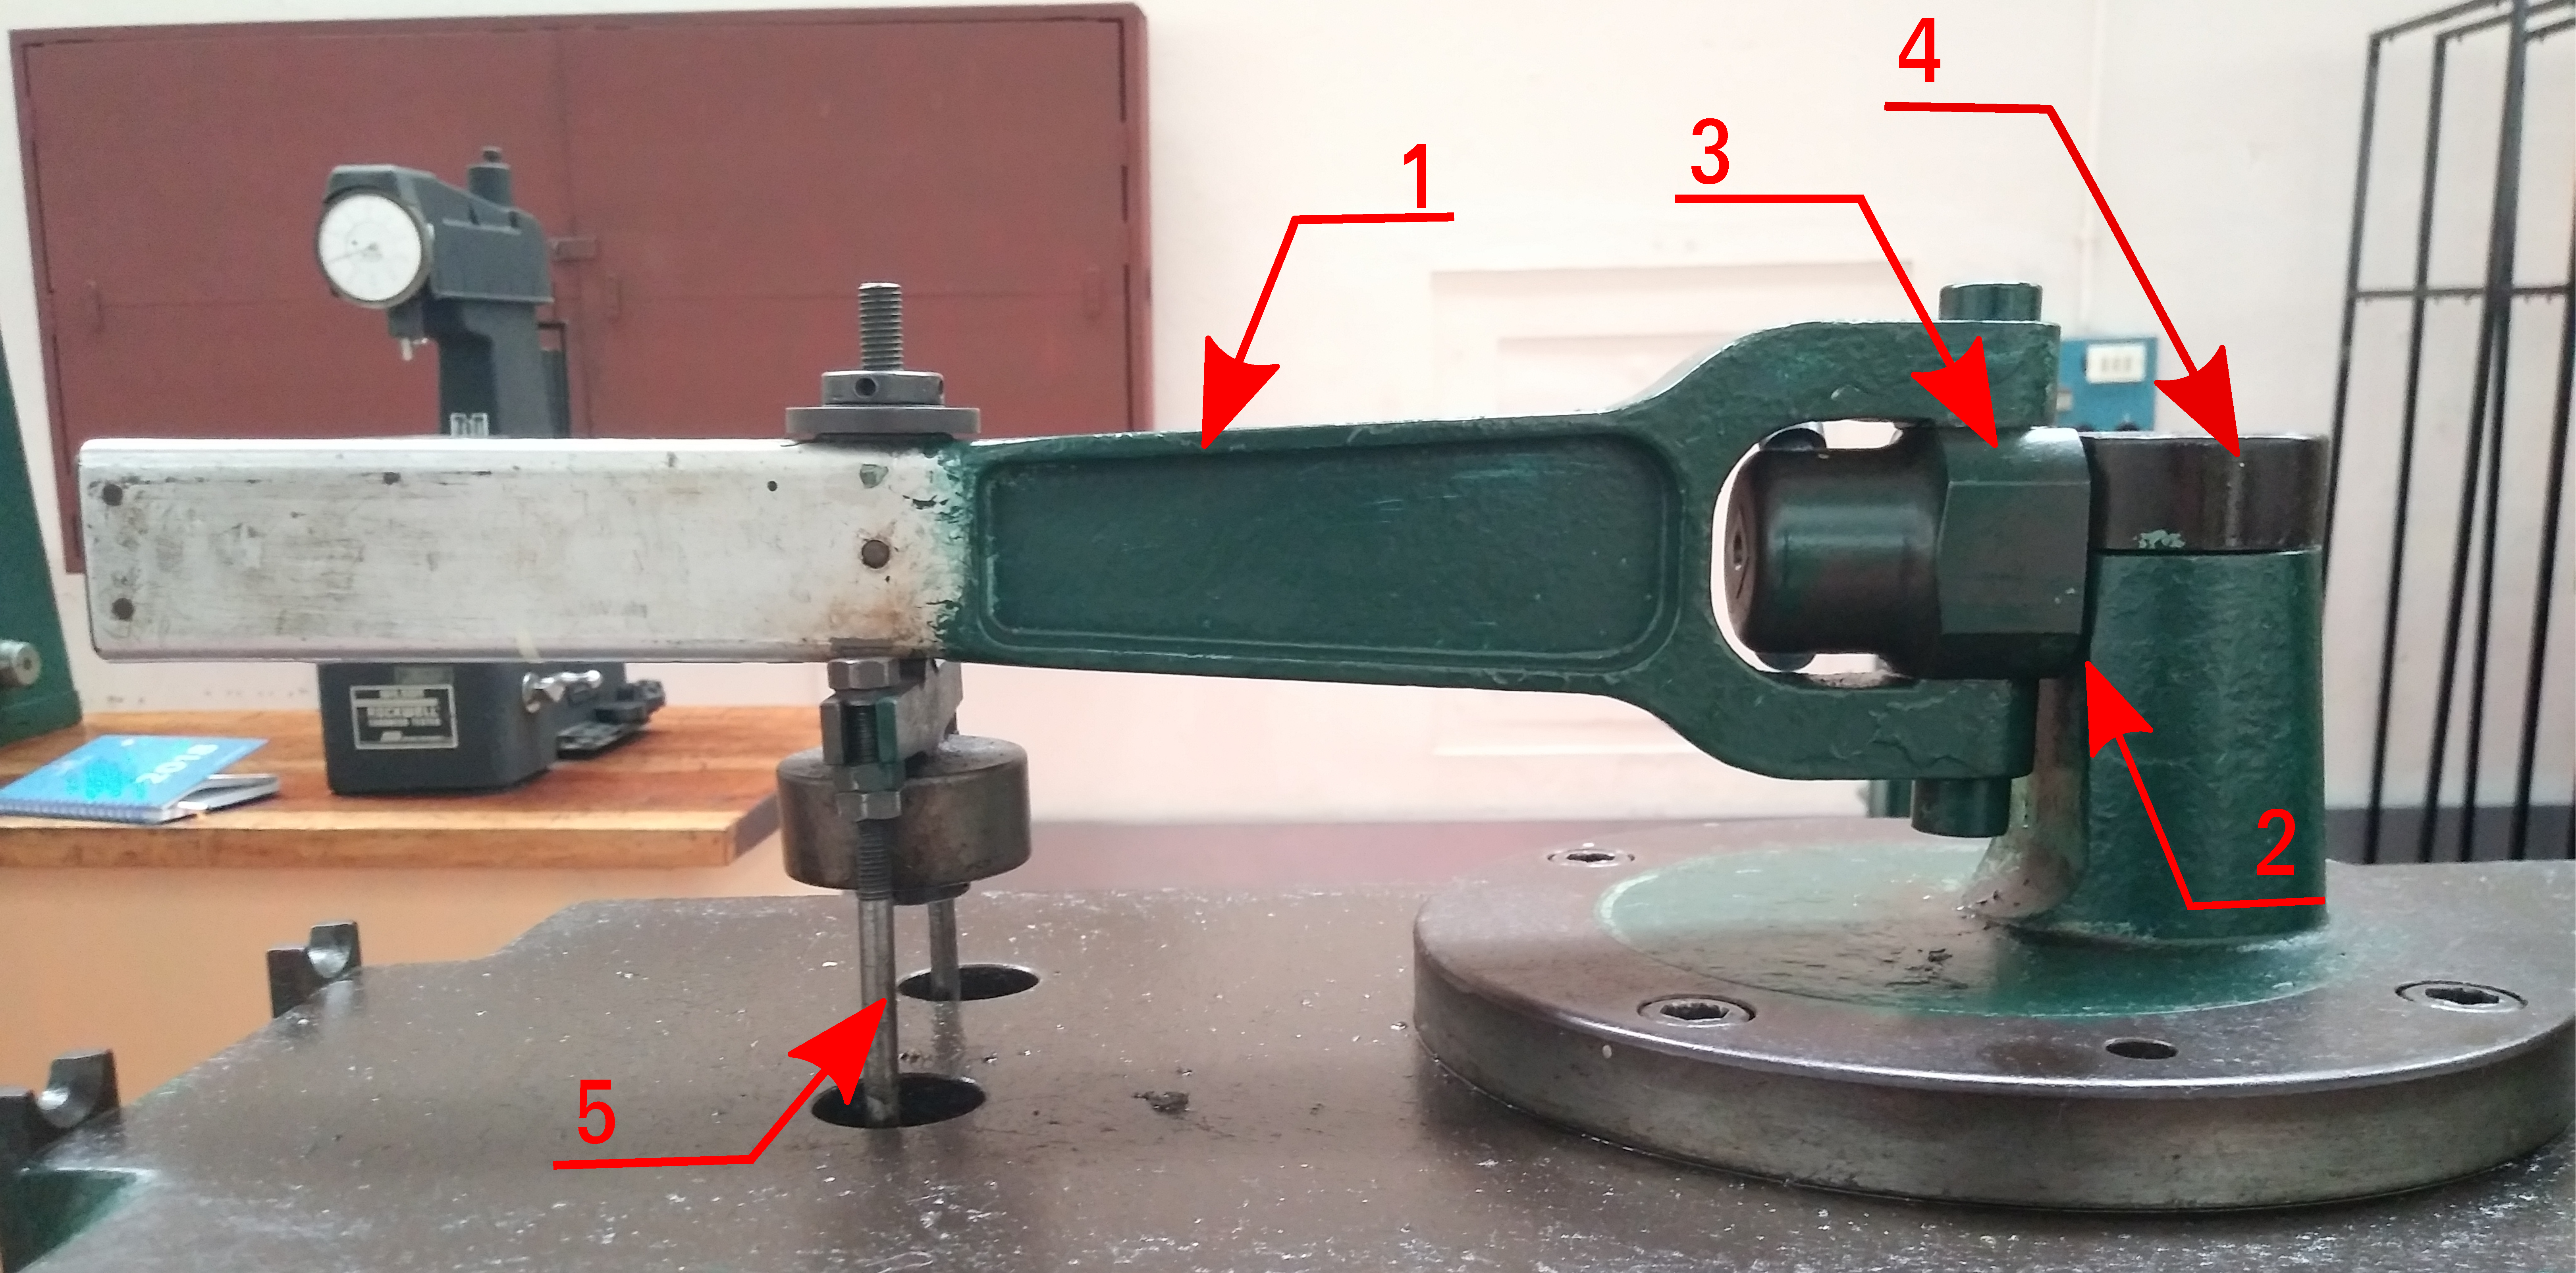
\includegraphics[width=\linewidth]{Imagenes/brazo_carga.pdf}
		\caption{Barra de carga y sus elementos}\label{fig:elementos_brazo}
	\end{subfigure}
	\begin{subfigure}{1\linewidth}
		\centering
		\includegraphics[width=\linewidth]{Imagenes/disco_barra.pdf}
		\caption{Disco desbalanceado en voladizo}\label{fig:elementos_disco}
	\end{subfigure}
\caption{En las imagenes (a) y (b) se enumeran los elementos que fueron considerados al modelar el sistema vibratorio. (1) Barra de carga. (2) Probeta ($k_2$), que se encuentra cubierta por ambas mordazas. (3) Mordaza sujeta al brazo de carga. (4) Mordaza empotrada a la máquina. (5) Barra de transmisión de la carga. (6) Disco desbalanceado. (7) Soportes de contrapeso. (8) Sistema de vigas en voladizo ($k_1$).}
\label{fig:elementos_modelo}
\end{figure}

\subsection{Modelo del sistema}
\label{sec:mod_sist}
Como se señaló, para poder crear un modelo del sistema y obtener soluciones, se realizaron simplificaciones y suposiciones que permiten llegar a una solución. Así, la fig. \ref{fig:diag_modelo} muestra el diagrama que se modelará con las ecuaciones de movimiento. Parte de estas simplificaciones es la exclusión de las fuerzas horizontales, en dirección de la coordenada $x$ de acuerdo a la referencia utilizada. Para esto, también es necesario quitarle los grados de libertad a la barra de transmisión de la carga y simplificar la carga producida por la rotación del disco, explicado en la sección siguiente. Por último, se asumirá que el movimiento angular del brazo de carga será lo suficientemente pequeño como linealizar la función trigonométrica del ángulo $\theta$, aproximándose $\sin(\theta) = \theta$ y $\cos(\theta)=1$.

\begin{figure}[h]
\centering
\includegraphics[width=0.9\linewidth, trim={5cm 2cm 10cm 1cm}, clip]{Imagenes/mach_diag.pdf}
\caption{Diagrama del modelo utilizado y el sistema de coordenadas.}
\label{fig:diag_modelo}
\end{figure}

Los sistemas de coordenadas $y(t)$ y $\theta (t)$ definen la posición y el movimiento del brazo de carga en cualquier instante $t$. Al ser independientes entre sí y no depender de ninguna restricción, es que las coordenadas generalizadas serán $q_1 = y$ y $q_2 = \theta$. A modo de conveniencia se establecerán las variables $y_1$ e $y_2$, las cuales describen el movimiento en ambos extremos del brazo.
\begin{gather}
	y_1(t) = y(t) - l_1\theta(t) \label{eq:y1}\\
	y_2(t) = y(t) + l_2\theta(t) \label{eq:y2}
\end{gather}
Si $t_0=0$, entonces cuando $y(t_0) = 0$ y $\theta(t_0) = 0$ la deformación en ambos resortes será cero, por lo tanto las variables $y_1$ e $y_2$ son equivalentes a la deformación de los resortes. La rigidez de cada resorte se denotarán como $k_1$, relativo a las vigas en voladizo, y $k_2$, relativo a la probeta.

Por otro lado, la velocidad de las coordenadas se definirán como $\dot{y}(t)$ y $\dot{\theta}(t)$ y, de manera análoga, la aceleración como $\ddot{y}(t)$ y $\ddot{\theta}(t)$. A partir de las ecuaciones \ref{eq:y1} y \ref{eq:y2} se obtiene que:
\begin{gather*}
	\dot{y_1}(t) = \dot{y}(t) - l_1\dot{\theta}(t) \quad ;\quad \ddot{y_1}(t) = \ddot{y}(t) - l_1\ddot{\theta}(t) \\
 	\dot{y_2}(t) = \dot{y}(t) + l_2\dot{\theta}(t) \quad ;\quad \ddot{y_2}(t) = \ddot{y}(t) + l_2\ddot{\theta}(t) 
\end{gather*}
La variable $M_a$ representa la masa total del disco, que se expresa como:
\begin{equation}\label{eq:m_a}
	M_a = M_d + m_1 + m_2
\end{equation}
Donde $M_d$ es la masa del disco y $m_1$ y $m_2$ la suma de los contrapesos colocados en cada soporte. 

Las constantes del brazo de carga, $M_b$ es la masa total del brazo de carga e $I_{gb}$ el momento de inercia con respecto al centro de masa. Las longitudes $l_1$ y $l_2$ corresponden a la distancia entre el centro de masa y la unión con la barra y la probeta, respectivamente. Por último, las constantes $c_1$ y $c_2$ son los amortiguamientos correspondientes a cada resorte.

\subsubsection{Modelo del disco}
Frente a la eliminación de las fuerzas horizontales del modelo, se simplificó la carga producida por el disco desbalanceado a una fuerza variable en el tiempo, que actúa solo en dirección vertical y es externa al sistema. Esta fuerza queda expresada de la siguiente forma:
\begin{equation}\label{eq:fza_gen}
	F_d(t) = M_a\, e_{ga}(\dot{\phi}^2 \sin\phi - \ddot{\phi} \cos\phi)
\end{equation}
La variable $e_{ga}$ corresponde a la excentricidad del centro de masa del disco provocada por el desequilibrio entre $m_1$ y $m_2$, el cual se detallará en la sección siguiente. También, la función $\phi$, con su respectiva velocidad y aceleración, es la coordenada angular del disco respecto al tiempo, la que será explicada en la sección \ref{sec:function_angle}.

\subsubsection{Ecuaciones de movimiento}
Utilizando el diagrama expuesto, entonces es posible escribir las ecuaciones que describen el movimiento del sistema utilizando el método de energía. Para esto, es necesario identificar los sistemas que actúan como parte de la energía cinética y potencial del sistema, además de las fuerzas externas que interactúan.

Se sabe que los elementos que actúan como resortes tienen el comportamiento de almacenar energía potencial, como se definió en la sección de rigidez. Por lo tanto, a partir de la ecuación \ref{eq:e_potelas}, expresa los elementos que interactúan en el sistema:
\begin{equation}
	U_k = \frac{1}{2} \left(k_1\cdot y_1^2 + k_2\cdot y_2^2\right)
\end{equation}
La energía potencial gravitatoria se obtiene al utilizar la ecuación \ref{eq:e_potgrav}, por lo tanto, se obtiene:
\begin{equation}
	U_g = g\cdot \left(M_a\, y_1 + M_b\, y\right)
\end{equation}
Por otro lado, la energía cinética se calcula según la ecuación \ref{eq:e_cinetica} para cada masa del sistema.
\begin{equation}
	T = \frac{1}{2} \left(M_a\, \dot{y_1}^2 + M_b\, \dot{y}^2\right)
\end{equation}
La energía disipada por el amortiguamiento viscoso se modela utilizando la ecuación \ref{eq:rayleigh_function}, llamada función de disipación de Reyleigh. 
\begin{equation}
	R = \frac{1}{2} \left(c_1\, \dot{y_1}^2 + c_2\, \dot{y_2}^2\right)
\end{equation}
Por último, la fuerza generalizada $Q_i$ es la fuerza variable de la ec. \ref{eq:fza_gen} proveniente del disco desbalanceado.\\ \\
Con esto, el método de Lagrange define al lagrangiano $L$ como la resta entre la energía cinética $T$ y la energía potencial total $U$, la cual según la ecuación \ref{eq:der_lag}, es la suma de la energía potencial elástica y gravitatoria. Así, la ecuación de energía para un sistema con amortiguamiento y forzado, a través del método de Lagrange es:
\begin{equation}
	\frac{d}{dt}\left(\frac{\partial L}{\partial \dot{q_i}}\right) - \frac{\partial L}{\partial q_i} = Q_i - \frac{\partial R}{\partial \dot{q_i}}
\end{equation}
\newpage
Al reemplazar y derivar cada término para cada coordenada generalizada, quedan las siguientes expresiones:
\begin{subequations}
\begin{align}
	M_b\, \ddot{y} + M_a\, \ddot{y_1} + k_1\, y_1 + k_2\, y_2 + M_a\, g + M_b\, g &= F_d(t) - c_1\, \dot{y_1} - c_2\, \dot{y_2} \\
	I_{gb}\, \ddot{\theta} - M_a\, y_1\, l_1 - k_1\, y\, l_1 + k_2\, y_2\, l_2 - M_a\, g\, l_1 &= F_d(t)\cdot l_1 + c_1\, \dot{y_1}\, l_1 - c_2\, \dot{y_2}\, l_2 
\end{align}
\end{subequations}

Al reemplazar las variables $y_1$ e $y_2$ y reacomodando los términos, se obtienen las dos ecuaciones de movimiento del brazo de carga:
\begin{subequations}
\begin{multline}\label{eq:mov_y}
	\ddot{y}(M_a + M_b) - \ddot{\theta}M_al_1 + k_1(y - l_1\theta) + k_2(y + l_2\theta) + \dots \\
	 M_a\, g + M_b\, g = F_d(t) - c_1(\dot{y} - l_1\dot{\theta}) - c_2(\dot{y} + l_2\dot{\theta}) 
\end{multline} 
\vspace{-17mm}
\begin{multline}\label{eq:mov_theta}
	\ddot{\theta}(I_{gb} - M_al_1) - \ddot{y}M_al_1 + k_1(y - l_1\theta)\cdot l_1 + k_2(y + l_2\theta)\cdot l_2 + \dots \\
	M_a\, g\, l_1 = F_d(t)\cdot l_1 + c_1(\dot{y} - l_1\dot{\theta})\cdot l_1 - c_2(\dot{y} + l_2\dot{\theta})\cdot l_2 
\end{multline}
\end{subequations}

Estas se pueden reescribir de forma matricial:

\begin{equation}\label{eq:mov_matriz}
\begin{split}
\begin{bmatrix}
	M_a + M_b	& -M_a\,l_1 \\
	-M_a\,l_1	& I_{gb} - M_a\,l_1^2
\end{bmatrix}
\begin{bmatrix}
	\ddot{y}\\
	\ddot{\theta}
\end{bmatrix} +
\begin{bmatrix}
	c_1 + c_2			& c_2\,l_2 - c_1\,l_1\\
	c_2\,l_2 - c_1\,l_1	& c_2\,l_2^2 - c_1\,l_1^2\\
\end{bmatrix}
\begin{bmatrix}
	\dot{y}\\
	\dot{\theta}
\end{bmatrix} + \dots \\
\begin{bmatrix}
	k_1 + k_2			& k_2\,l_2 - k_1\,l_1\\
	k_2\,l_2 - k_1\,l_1	& k_2\,l_2^2 - k_1\,l_1^2
\end{bmatrix}
\begin{bmatrix}
	y\\
	\theta
\end{bmatrix} =
\begin{bmatrix}
	F_d(t) - g(M_a + M_b)\\
	F_d(t)\cdot l_1 + g\,M_a\,l_1
\end{bmatrix}
\end{split}
\end{equation}

\subsection{Cálculo de constantes características del sistema}
 
\subsubsection{Rigidez y amortiguamiento} Las constantes de rigidez de las barras en voladizo $k_1$ y de la probeta $k_2$ se obtuvieron simulando su deformación elástica a través del software Inventor Autodesk. Para ello, se empotraron en un extremo y se les aplicaron distintas niveles de carga en el otro. Con los datos obtenidos fue posible ajustar una curva en una gráfica de deformación versus fuerza aplicada, donde la pendiente obtenida es la constante de rigidez del elemento. 

Además, se realizaron cálculos para comprobar el orden de magnitud obtenido a través del software. Para esto se utilizó la ecuación \ref{eq:k_cantilever}, para una viga en voladizo. La tabla \ref{tab:k_valor} muestra los resultados de ambos métodos.
\begin{table}[h]
\centering
\begin{tabular}{ccc}
\hline
Método & Barras en voladizo & Probeta \\ \hline
Simulación Inventor & $9.889\cdot 10^4$ [N/m] & $1.809\cdot 10^6$ [N/m] \\
Cálculo & $9.216\cdot 10^4$ [N/m] & -- \\ \hline
\end{tabular}
\caption{Valores obtenidos mediante un modelo de elementos finitos y por media de la ec. \ref{eq:k_cantilever} de la rigidez de las vigas en voladizo y la probeta de acero}
\label{tab:k_valor}
\end{table}
Los datos utilizados en el modelo corresponden a los obtenidos por simulación.

Por otro lado, los valores de $c_1$ y $c_2$ se estimaron de manera cualitativa, visualizando la curvas de $y(t)$ y $\theta(t)$ para buscar que la vibración inicial se disipara antes del inicio de la función de aceleración del disco. Así, los valores utilizados son:
\begin{itemize*}
	\item $c_1= 100$
	\item $c_2= 100$ 
\end{itemize*}
\subsubsection{Segundo momento de área de la probeta y las vigas en voladizo}
El segundo momento de área o segundo momento de inercia, se calculó para obtener la rigidez de los dos elementos anteriores. Para el segundo momento de inercia de la probeta se utilizará la sección transversal de la sección media de la probeta. Así, su valor es:
\begin{equation}
	\bar{I}_p = \frac{\pi \cdot d^4}{32} = 330,994\: \text{mm}^4
\end{equation}
Para las vigas en voladizo, el segundo momento de área se calculó en la sección \ref{sec:mediciones_met}, el cual es:
\begin{equation}
	\bar{I}_{barras} = 5.67 \cdot 10^{-8} \text{m}^4
\end{equation}
\subsubsection{Momento de inercia del brazo de carga}
El momento de inercia del brazo de carga se obtuvo a través del modelo CAD del mismo, respecto a su centro de masa. Su valor es $I_{gb} = 5.6718\cdot 10^{-8} \text{ kg}\cdot \text{m}^2$ . 

\subsubsection{Longitud, masa y módulo de elasticidad}
Los elementos del sistema explicados en la sección \ref{sec:mod_sist}, dimensiones y propiedades que se midieron como parte del levantamiento de informacioń. 
\subparagraph{\textit{Brazo de carga.}}
La distancia correspondiente a cada extremo respecto al centro de masa es:
\begin{itemize*}
	\item $l_1=$ 42,43 mm
	\item $l_2=$ 158,07 mm
\end{itemize*}
Además, la masa $M_b$ corresponde a la masa medida del brazo de carga, como se especificó en la sección \ref{sec:mediciones_met}:
\begin{itemize*}
	\item $M_b=$ 2,305 Kg
\end{itemize*}
\subparagraph{\textit{Masa del disco}.}
Por otro lado, la masa $M_a$ como se señaló en la ecuación \ref{eq:m_a}, corresponde a la suma de tres elementos. El primero de ellos, la masa del disco, tiene un valor de:
\begin{itemize*}
	\item $M_d=$ 19,2029 kg
\end{itemize*}
Los valores correspondientes a $m_1$ y $m_2$ son variables y pueden ir desde 0 g hasta 92,3469 g de acuerdo a la configuración escogida. Las distintas combinaciones y valores que pueden tener se encuentran en la tabla del anexo \ref{ch:anexo_b}.
\subparagraph{\textit{Módulo de elasticidad de la probeta}.}
Corresponde al del material de la probeta que actualmente se utiliza. Al ser acero, su valor es:
\begin{itemize*}
	\item $E_p=$ 200 GPa
\end{itemize*}
\subsubsection{Excentricidad}
La excentricidad del centro de masa $e_{ga}$ se calculó utilizando los datos del disco, la distancia de los soportes y la configuración de masas. Por lo tanto, se define como:
\begin{equation}
	e_{ga} = \frac{R_d\cdot (m_1 - m_2)}{(m_1 + m_2 + M_d)}
\end{equation}
\subsection{Función de aceleración del disco}
\label{sec:function_angle}
La filosofía detrás de la función $\phi$ es poder controlar el tiempo de retraso de la rotación del disco, que se designará como $T_i$, y suavizar la aceleración del mismo hasta que llega a la velocidad de rotación máxima $\omega_{max}$. Para esto, la función de la aceleración $\ddot{\phi}(t)$ se formuló como una función por partes, como se ve en la fig. \ref{fig:anglepp}, donde el parámetro $T$ indicará la suavidad con la que es acelerado el disco. Estas tres constantes, $T_i$, $\omega_{max}$ y $T$, son valores de entrada que se eligen dependiendo de los resultados que se deseen.
\begin{figure}[h]
\centering
\includegraphics[width=0.9\linewidth, trim={6.5cm 2cm 10cm 2cm},clip]{Imagenes/anglepp_function.pdf}
\caption{Función por parte de la aceleración del disco}
\label{fig:anglepp}
\end{figure}
Así, la función $\ddot{\phi}$ adquiere la forma:
\[ \ddot{\phi}(t) =
\begin{dcases}
	0																		&	t \leq T_i \\
	\left(\frac{\omega_{max}}{T^2}\right)\left(t - T_i\right)				&	T_i < t \leq T_i + T\\
	\left(\frac{\omega_{max}}{T}\right)\left(2 - \frac{t - T_i}{T}\right)	&	T_i + T < t \leq T_i + 2T\\
	0																		&	T_i + 2T < t\\
\end{dcases} 
\]
Para obtener la función de la velocidad $\dot{\phi}(t)$ se debe integrar la función anterior, donde las constantes de integración se obtienen por los valores extremos conocidos, es decir, $\dot{\phi}(T_i) = 0$ y $\dot{\phi}(T_i + 2T) = \omega_{max}$. Entonces, la función se define como:
\[ \dot{\phi}(t) =
\begin{dcases}
	0																												&	t \leq T_i \\
	\left(\frac{\omega_{max}}{2T^2}\right)\left(t^2 - 2T_i\cdot t + T_i^2\right)									&	T_i < t \leq T_i + T\\
	\left(\frac{\omega_{max}}{T}\right)\left(2t - 2T_i - 3T + \frac{4T^2 - T_i^2 - t^2 + 2T_i\cdot t}{2T}\right)	&	T_i + T < t \leq T_i + 2T\\
	\omega_{max}																									&	T_i + 2T < t\\
\end{dcases} 
\]
El resultado de la función $\dot{\phi}(t)$, se muestra en la fig. \ref{fig:anglep}.
\begin{figure}[h]
\centering
\includegraphics[width=0.85\linewidth, trim={7cm 5cm 15cm 6cm},clip]{Imagenes/anglep_function.pdf}
\caption{Función por parte de la velocidad angular del disco}
\label{fig:anglep}
\end{figure}

Para concluir, se repite el mismo procedimiento anterior para obtener la función $\phi (t)$, sin embargo, para conocer las constantes de integración, los puntos conocidos serán cuando $\phi(T_i) = 0$ y la igualdad de la función en el punto $T_i + T$. Así, es obtiene:
\[ \phi (t) =
\begin{dcases}
	0																									&	t \leq T_i \\
	\left(\frac{\omega_{max}}{6T^2}\right)\left(t^3 - 3T_i\cdot^2 t + 3T_i^2\cdot t - T_i^3\right)		&	T_i < t \leq T_i + T\\
	\Phi_3																								&	T_i + T < t \leq T_i + 2T\\
	\omega_{max}\, t - \omega_{max}(T + T_i)															&	T_i + 2T < t\\
\end{dcases} 
\]
La función $\phi_3$ correspondiente al dominio cuando $t$ es mayor a $T_i + T$ y menor a $T_i  + 2T$ es:
\begin{multline*}
\Phi_3 = \left(\frac{\omega_{max}}{T}\right)\left(t^2 - 2T_i\cdot t - 3T\cdot t + \left(\frac{1}{2T}\right)\left(4T^2\cdot t - T_i^2\cdot t - \frac{t^3}{3} + T_i\cdot t^2\right)\right)\dots \\
 + \left(\frac{1}{6T^2}\right) \left(2\omega_{max}T^3 + 6\omega_{max}T^2T_i + 6\omega_{max}T\,T_i + \omega_{max}T_i^3\right)
\end{multline*}

Para el desarrollo de este trabajo, el tiempo de retraso de la aceleración del disco será de $T_i=2$, instante en el que la barra se encuentra en un estado de reposo en consecuencia del valor de los amortiguamientos $c_1$ y $c_2$. Por otro lado, se definirá $T = 2,5$ como un valor que logra suavizar la aceleración, pero sin dilatar en exceso la llegada al punto de velocidad máxima. Finalmente, $\omega_{max}\,$ el valor por defecto corresponderá a la velocidad actual de la máquina de 25 [rad/s] (1500 revoluciones por minuto), sin embargo, este se puede variar dependiendo de los resultados que se deseen obtener. 

\subsection{Solución del modelo}
Para resolver el sistema de ecuaciones \ref{eq:mov_matriz}, se utilizará el solver de ecuaciones diferenciales ordinarias de MATLAB, ode45, que se basa en el método de Runge-Kutta con un espacio de tiempo variable para resolver sistemas de EDOs de primer orden y con condición inicial. \cite{ode45}

Para resolverlo es necesario ingresar datos de entrada al sistema. Para esto, primero se debe escoger la configuración de contrapesos $m_1$ y $m_2$ a partir de la tabla de cargas. El segundo de ellos es el tiempo que define los límites de integración de la función, el que se escogerá según la cantidad de información que se desee obtener. En tercer lugar, se deben ingresar los valores de la condición inicial correspondiente a cada variable. Por último, es opcional añadir valores de tolerancia relativa y absoluta.

Al ser el sistema de ecuaciones de segundo orden, es necesario realizar un cambio de variables para poder resolverlo. Se añadirán las nuevas variables $\gamma$ y $\beta$, realizando la siguiente derivación:
\[ \left. 
\begin{array}{ll}
	\gamma = \dot{y}\\
	\beta = \dot{\theta}\\
\end{array}
\right\}
\begin{array}{ll}
	\ddot{y} &= \dot{\gamma}\\
	\ddot{\theta} &= \dot{\beta}\\
\end{array}\]
Para esto es necesario despejar los valores de $\ddot{y}$ y $\ddot{\theta}$, entonces la función a resolver estará dada por los elementos $(\gamma, \dot{\gamma}, \beta, \dot{\beta})$ y los resultados obtenidos serán $(y, \dot{y}, \theta, \dot{\theta})$. A partir de los resultados, es posible calcular la fuerza sobre la probeta utilizando la deformación $y_2$ y la constante de rigidez $k_2$.
\begin{equation}\label{eq:fuerza_probeta}
	F(t) = k_2 \cdot y_2 = k_2(y + l_2\theta)
\end{equation}

\subsection{Matriz de carga sobre la probeta según velocidad del motor}
Una vez que se puede resolver el sistema de ecuaciones para un configuración y velocidad del motor específica, entonces es posible obtener una matriz del valor de la fuerza máxima ($F_{max}$), media ($F_m$) y su amplitud ($F_a$) para cada una de las configuraciones existentes en la tabla de carga a una velocidad angular $\,\omega_{max}\,$ determinada.

Para esto se itera la solución anterior para cada una de las 201 configuraciones de contrapeso existentes para distintas velocidades. De estas iteraciones se almacenan los valores de $F_{max}$, $F_m$, $F_a$ y la diferencia de masa de los contrapeso $\Delta m$. 

\subsubsection{Carga máxima, media y amplitud}
La información que se busca de estos resultados corresponde a la carga que es producto de la fuerza del disco desbalanceado sobre la probeta, es decir, $F(t)$. Producto del comportamiento con el que se diseñó el modelo donde el sistema se deja caer hasta su posición de equilibrio,  se utiliza una variable auxiliar $F_{aux}$ que extrae los datos de $F(t)$ desde el inicio de la aceleración angular del disco hasta el final de la integración para evitar que las fuerzas de la transición entre la posición inicial y el reposo den resultados incorrectos. Así, la carga máxima, media y la amplitud se definen:
\begin{gather} 
	F_{max} = \text{max}(|F_{aux}|) \label{eq:f_max}\\
	F_m = \frac{\text{max}(F_{aux}) + \text{min}(F_{aux})}{2} \label{eq:f_m}\\
	F_a = \frac{\text{max}(F_{aux}) - \text{min}(F_{aux})}{2} \label{eq:f_a}
\end{gather}

\section{Simulación de carga máxima}
Con los datos de la carga máxima $F_{max}$, obtenidos a partir de la solución del modelo expuesto anteriormente, para cada combinación de contrapesos, se realizará un análisis estático de los esfuerzos asociados a cada configuración, en otras palabras, se buscará relacionar cada combinación con los esfuerzos respectivos a una velocidad angular máxima $\omega_{max}$ de 25 [rad/s]. Para esto, se simulará la probeta a través del software de elementos finitos ANSYS con el fin de obtener el esfuerzo máximo equivalente (o de von Mises), el esfuerzo máximo cortante, normal y sus respectivas deformaciones. Finalmente, se compararán los resultados de este análisis con la tabla de cargas existente. Debido a lo alto de las cargas obtenidas, sólo se considerarán las simulaciones que lleven a la probeta lo más cercano al punto de esfuerzo último, por lo tanto, la probeta será sometida a 77 cargas distintas, donde la carga 77 excede el esfuerzo último del material.

\newpage

\subsection{Tipo de simulación}
Al llevar a la probeta a cargas que sobrepasan el esfuerzo de fluencia del material, es necesario utilizar un modelo elasto-plástico para el correcto desarrollo de la simulación. En consecuencia, se utilizará el modelo de plasticidad multilineal de endurecimiento isotrópico (MISO), utilizado comúnmente para el análisis en grandes deformaciones. Este modelo se debe alimentar con los datos de distintos puntos de esfuerzo y deformación plástica real de un ensayo de tracción del material, creando una curva con los distintos puntos introducidos donde la primera pendiente es la zona elástica. Este modelo no permite que en la zona plástica hayan pendientes más grandes que en la zona elástica ni pendientes negativas. 

\subsection{Propiedades del material}
\subsubsection{Medición de la dureza}
Para conocer a que acero correspondía el utilizado en las probetas que existen actualmente, se realizó un ensayo de dureza del material. Este ensayo se realizó en los laboratorios de tecnología mecánica en un medidor de dureza de escala Rockwell, marca Wilson del año 1970. Se realizaron tres mediciones en distintas caras de la probeta en la configuración de Rockwell B, de las cuales se obtuvieron:
\begin{gather*}
	H_1 = 54 \text{ HRB} \qquad \qquad H_2 = 56 \text{ HRB} \qquad \qquad H_3 = 54 \text{ HRB}
\end{gather*}
Por lo tanto se considerará una dureza del material de $H = 54.6$ HRB. Sin embargo, debido a la antiguedad del equipo, la norma \textbf{ISO 18265:2013 - Conversion of hardness values} \cite{ISO18265} establece que se debe realizar una corrección a estos valores debido a una actualización en el indentador utilizado y una reducción del tiempo de fuerza aplicado durante la medición. De esta forma, la dureza final promedio que se obtuvo corresponde a $H = 54.8$ HRB. Por último, en base a esta misma norma, se puede realizar la conversión a dureza Vickers, siendo $H = 98.3 \approx 100$ HV y obtener el valor de un esfuerzo último de referencia $\sigma_u(\texttt{@}\text{HV}=100) = 315 \; \text{MPa}$.

\subsubsection{Curva de esfuerzo-deformación del acero}
A causa de lo bajo del valor de dureza obtenido, sumado al hecho que en los únicos aceros utilizados en el laboratorio son SAE 1020 y 1040, es que se decide tomar las propiedades mecánicas del primero de estos. Los datos utilizados se obtuvieron de un ensayo de tracción realizado por la Universidad de Washington de un acero SAE 1020 laminado en caliente (AISI 1020 HR)\cite{1020data}. Estos datos contienen la fuerza aplicada, la deformación sufrida y el diámetro original de la probeta, para los cuales se utilizaron las ecuaciones \ref{eq:true_esf} y \ref{eq:true_strain} para obtener los esfuerzos y deformaciones reales y el factor de corrección de Bridgman (ec. \ref{eq:bridgman}). En la fig. \ref{fig:esf_realing}, se pueden apreciar la curva original de esfuerzo-deformación ingenieril y la curva de esfuerzo-deformación real. 

\begin{figure}[h]
\centering
\includegraphics[width=1\linewidth, trim={2cm 6cm 2cm 5cm},clip]{Imagenes/esf_real_ing.pdf}
\caption{Curva de esfuerzo-deformación del material AISI 1020 en valores ingenieriles y reales.}
\label{fig:esf_realing}
\end{figure}

Sin embargo, debido a las características del modelo MISO, se deben utilizar exclusivamente los puntos de la zona plástica y estos no pueden tener una pendiente menor a cero entre dos puntos ingresados, por lo tanto, la tabla \ref{tab:esfdef_util} muestra los datos utilizados. Por otra parte, el último punto corresponde al esfuerzo de ruptura, pero no se ingresó un modelo de ruptura al no ser relevante para el trabajo. 

Por último, para la deformación elástica se usará un modulo de elasticidad $E =$ 200 GPa, el esfuerzo de fluencia es $\sigma_y=$ 293,5 MPa y el esfuerzo último $\sigma_u =$ 418,5 MPa.
\begin{table}[h]
\centering
\begin{tabular}{@{}cc@{}}
\toprule
\begin{tabular}[c]{@{}c@{}}Deformación unitaria plástica real\\ $\tilde{\varepsilon}$ (-)\end{tabular} & \begin{tabular}[c]{@{}c@{}}Esfuerzo real corregido\\ $\tilde{\sigma}_B$ (MPa)\end{tabular} \\ \midrule
0 & 293,5 \\
0,0462 & 334,3 \\
0,1157 & 418,5 \\
0,1949 & 465,3 \\
0,2079 & 469,8 \\
0,3547 & 505,0 \\
0,5271 & 540,9 \\
0,7190 & 576,2 \\
0,9278 & 611,5 \\
1,0877 & 649,1 \\ \bottomrule
\end{tabular}
\caption{Datos utilizados del ensayo de esfuerzo-deformación del acero AISI 1020 HR en el modelo MISO.}
\label{tab:esfdef_util}
\end{table}

\subsection{Generación de la malla}
\label{sec:gen_malla}
Producto de lo irregular de la geometría de la probeta y la importancia que tienen para los resultados la zona media, por sobre los agarres, es que se opta por mallar para cada sección. En configuración generaldel mallado se utilizaron parámetros que buscan mejorar su calidad\footnote{La definición de cada opción se encuentra en el manual de ANSYS. \cite{sharcnet_mesh}}.

\begin{itemize*}
	\item Sizing
		\begin{itemize*}
			\item Transition: Slow
			\item Span Angle Center: Fine
		\end{itemize*}
	\item Quality
		\begin{itemize*}
			\item Error Limits: Aggressive Mechanical
			\item Targer Quality: 1 (-)
			\item Smoothing: High
		\end{itemize*}
\end{itemize*}

Para obtener los resultados de una malla que se adaptara a los requisitos, se utiliza el \textit{body sizing} y el \textit{face sizing}. Así, la configuración utilizada para cada sección es la siguiente\footnote{Ibíd.}:
\begin{itemize*}
	\item Probeta completa
		\begin{itemize*}
			\item Body sizing
			\item Tamaño elemento: 0,01 mm
		\end{itemize*}
	\item Sección intermedia (fig. \ref{fig:zona_media})
		\begin{itemize*}
			\item Face sizing
			\item Tamaño elemento: 0,001 mm
		\end{itemize*}
	\item Sección transversal media (fig. \ref{fig:cara_corte})
		\begin{itemize*}
			\item Face sizing
			\item Tamaño elemento: 0,0001 mm
		\end{itemize*}
\end{itemize*}

\newpage

Con esta configuración la malla está compuesta por 951.151 nodos y 684.131 elementos. Los valores promedios de los parámetros que indican la calidad de la malla, expuestos en la sección \ref{sec:gen_malla}, se muestran en la tabla \ref{tab:cal_malla}.
\begin{table}[h]
\centering
\begin{tabular}{@{}lc@{}}
\toprule
Parámetro de calidad & Valor promedio \\ \midrule
Calidad del elemento & $0.839$ \\
Relación de aspecto & $1.817$ \\
Calidad ortogonal & $0.772$ \\
Oblicuidad & $0.22667$ \\ \bottomrule
\end{tabular}
\caption{Valores promedios de los parámetros de calidad de la malla utilizada en la probeta.}
\label{tab:cal_malla}
\end{table}
%\begin{align*}
%	\bullet \ &\text{Calidad del elemento} &=\quad	 &0.839 	\\
%	\bullet \ &\text{Relación de aspecto}  &=\quad 	 &1,817 	\\
%	\bullet \ &\text{Calidad ortogonal} 	 &=\quad 	 &0,772 	\\
%	\bullet \ &\text{Oblicuidad} 			 &=\quad	 &0,22667
%\end{align*}

Estos valores muestran que la malla utilizada es aceptable. Al utilizar la tabla \ref{tab:skewness} como referencia, el valor de oblicuidad nos indica que la malla se encuentra en el rango ``\textit{Excelente}''.

\begin{figure}[t]
\centering
	\begin{subfigure}{0.5\linewidth}
		\centering
		\includegraphics[width=0.82\linewidth]{Imagenes/zona_media.PNG}
		\caption{}\label{fig:zona_media}
	\end{subfigure}%
	\begin{subfigure}{0.5\linewidth}
		\centering
		\includegraphics[width=0.6\linewidth]{Imagenes/cara_corte.PNG}
		\caption{}\label{fig:cara_corte}
	\end{subfigure}%
\caption{La zona verde de la imagen (a) corresponde a la zona intermedia de la probeta y la zona azul de la imagen (b) a la sección transversal en la mitad de la probeta.}
\label{fig:zona_probeta}
\end{figure}

\begin{figure}[p]
\centering
	\begin{subfigure}{0.5\linewidth}
		\centering
		\includegraphics[width=1\linewidth]{Imagenes/mgen_iso.png}
		\caption{}\label{fig:mgen_iso}
	\end{subfigure}%
	\begin{subfigure}{0.5\linewidth}
		\centering
		\includegraphics[width=1\linewidth]{Imagenes/mdet_iso.png}
		\caption{}\label{fig:mdet_iso}
	\end{subfigure}
	\par\bigskip
	\par\bigskip
	\begin{subfigure}{0.5\linewidth}
		\centering
		\includegraphics[width=0.9\linewidth]{Imagenes/mcorte.png}
		\caption{}\label{fig:mcorte}
	\end{subfigure}%
		\begin{subfigure}{0.5\linewidth}
		\centering
		\includegraphics[width=0.7\linewidth]{Imagenes/mcorte_det.png}
		\caption{}\label{fig:mcorte_det}
	\end{subfigure}
	\par\bigskip
\caption{(a) Vista isométrica general de la malla. (b) Detalle en isométrico de la zona media y la sección transversal. (c) Malla de la sección transversal media. (d) Detalle de la malla de la sección transversal media.}
\label{fig:malla}
\end{figure}


\newpage

\subsection{Configuración de la simulación estática}
\subsubsection{Condiciones de contorno}
El doble empotramiento al cual está sometida la probeta se aplicará restringiendo el movimiento en cada cara de uno de sus extremos. Utilizando la fig, \ref{fig:cond_borde} como referencia, las caras amarilla se encuentran restringidas de desplazamiento en el eje normal a su plano. Así, ambas caras paralelas al plano $xz$ tienen una restricción de desplazamiento de $\Delta y = 0$, las caras del plano $xy$ están restringidas de desplazamiento en el eje $z$ con $\Delta z = 0$ y la cara posterior del plano $yz$ su desplazamiento es $\Delta x = 0$.

Por otro lado, el otro extremo empotrado se le aplicarán las cargas máximas que se obtuvieron del modelo del sistema vibratorio, $F_{max}$. Sin embargo, no se aplicará como una carga puntual, sino como una presión sobre la cara roja de la probeta, según la imagen \ref{fig:cond_borde}. Para esto, se transformará la carga puntual a presión utilizando la relación:
\begin{equation}\label{eq:p_max}
	P_{max} = \frac{F_{max}}{A_{cara,l}}
\end{equation}
Donde $P_{max}$ es la presión aplicada sobre la cara y $A_{cara,l}$ el área de la cara lateral sobre el cual se aplica la carga, es decir la sección roja. Al medir esta área a través del modelo CAD, se obtiene $A_{cara,l} = 402.792 \text{ mm}^2$

\begin{figure}[]
\centering
\includegraphics[width=0.7\linewidth]{Imagenes/cond_borde.png}
\caption{Condiciones de contorno aplicadas en la probeta. Las caras amarillas representan las restricciones de desplazamiento y la cara roja la presión aplicada.}
\label{fig:cond_borde}
\end{figure}

\newpage

\subsubsection{Selección de elementos}
Dado que los esfuerzos máximos se encuentran en la sección media de la probeta, los resultados de la simulaciones se tomarán en los puntos específicos P, Q y R, cuya ubicación es mostrada en la fig. \ref{fig:diag_pqr}. Para esto, se seleccionarán los elementos que están en esa ubicación para posteriormente graficar sus resultados respecto a cada carga.

\begin{figure}[h]
\centering
\includegraphics[width=0.3\linewidth]{Imagenes/diagelem_pqr.pdf}
\caption{Ubicación de los elementos seleccionados}
\label{fig:diag_pqr}
\end{figure}

\subsubsection{Obtención de resultados}
En base a los elementos seleccionados, los resultados que se necesitan son:
\begin{itemize*}
	\item Esfuerzo equivalente o de von Mises ($\sigma_{vm}$)
	\item Esfuerzo máximo cortante ($\tau_{max}$)
	\item Esfuerzo máximo normal en dirección \textit{x} ($\sigma_{x}$), según referencia de la fig. \ref{fig:cond_borde}.
	\item Deformación unitaria equivalente total ($\varepsilon_{vm,t}$)
	\item Deformación unitaria normal elástica ($\varepsilon_{x}$),  según referencia de la fig. \ref{fig:cond_borde}.
\end{itemize*}

Además, a modo de referencia se utilizarán los resultados globales:
\begin{itemize*}
	\item Esfuerzo equivalente
	\item Deformación en dirección \textit{y}, según referencia de la fig. \ref{fig:cond_borde}
\end{itemize*}

%
\chapter{Análisis y Resultados}

\section{Levantamiento de información}
Por medio del levantamiento de información es posible hacer un pequeño análisis del estado actual y los datos obtenidos. Por un lado, la estructura actual responde a la necesidad de colocar la máquina en una ubicación transitoria, debido a los trabajos realizados en el piso del laboratorio durante el año 2012. Por lo mismo, no está diseñada para la operación de la máquina bajo ningún contexto por los peligros que conlleva. Aún cuando esta podría ser modificada, se desconocen las características y propiedades de la especie maderera con la que fue fabricada, lo que obliga a diseñar y construir un nuevo soporte para la máquina. 

Por otra parte, la información obtenida de la máquina de fatiga da cuenta de tres puntos importantes. La antigüedad de sus componentes y la tecnología utilizada afecta directamente en su mantenimiento ante la dificultad de encontrar piezas de repuesto, debido a que las dimensiones de sus componentes, como la polea y la correa, se encuentran fuera de catálogo o de las dimensiones de fabricación de los proveedores. También la obsolescencia de la tecnología afecta su mantenimiento, siendo difícil poder encontrar no sólo las piezas de repuesto, sino que también personas que estén técnicamente calificadas. En segundo lugar, la máquina fue fabricada con estándares o líneas de desarrollo propias de la época, como sería esperable, las cuales no evolucionaron en la misma dirección de que los estándares actuales de ensayo a fatiga, dificultando la comparación de los resultados obtenidos. Finalmente, la robustez del diseño, la cual se puede apreciar fácilmente en la dimensiones de la estructura exterior de la máquina, tiene la dualidad de proveer un armazón macizo y duradero sobre el cual trabajar, sin embargo, resulta ser una estructura difícil de modificar por esta misma razón.

En lo relativo a la exactitud de los datos obtenidos, la imposibilidad de desarmar gran parte de la máquina afectaron la precisión de las mediciones realizadas, sobre todo en partes específicas. Así, las dimensiones y la geometría de las barras de acero tuvieron que ser simplificadas ante la imposibilidad de tomar medidas en la unión barra-disco. Por la misma razón, la masa del disco desbalanceado, calculada a través de la deflexión de las barras de acero, incluye los errores de la medición anterior sumado a la masa de otros elemento que no son parte de la fuerza provocada por el desequilibrio del disco en rotación. Ante esto, surge la necesidad de poder desarmar la máquina para poder estudiarla con mayor detenimiento, obteniendo información que sea más precisa de sus elementos como también información útil para poder actualizar componentes que mejoren su desempeño y mantenibilidad. 
 
\section{Diseño de la estructura}
\subsection{Diseño en acero}
A partir de las ecuaciones \ref{eq:reaccion_acero}, \ref{eq:mtofleca_acero} y \ref{eq:esfmax_acero}, expuestas en la sección de diseño en acero en metodología, se probó de forma iterativa para distintas dimensiones del acero A270ES, su comportamiento bajo la carga estática. Como se señaló anteriormente, sólo se tomó en consideración pletinas de un ancho de 100 mm debido al espaciamiento necesario entre los pernos. Los resultados que se obtuvieron se encuentran en la siguiente tabla:

\begin{table}[h]
\centering
\resizebox{\textwidth}{!}{%
\begin{tabular}{@{}ccccccc@{}}
\toprule
N$^{\circ}$ & Dimensiones {[}mm{]} & I {[}mm$^4${]} & $R_A$ {[}N{]} & $M_A$ {[}Nm{]} & $\sigma_{max,pl}$ {[}MPa{]} & Factor de Seguridad {[}-{]} \\ \midrule
1 & 100x10 & 8333,33 & 23,87 & 2,46 & 60,88 & 4,43 \\
2 & 100x6 & 1800 & 14,32 & 1,48 & 167,46 & 1,61 \\
3 & 100x5 & 1041,66 & 11,95 & 1,23 & 240,56 & 1,12 \\
4 & 100x8 & 4266,66 & 19,09 & 1,97 & 94,66 & 2,85 \\ \bottomrule
\end{tabular}%
}
\caption{Tabla aceros}
\label{tab:itest_acero}
\end{table}

Con esta información en consideración, se comprobará su comportamiento bajo las cargas dinámicas, descartando el acero número 1 por estar sobredimensionado. Utilizando la ecuación \ref{eq:mtofat_acero} se obtiene que el momento provocado por la carga alternante es $M_{a,pl,A} =$ 50,42 [Nm]. De esta manera, al aplicar las ecuaciones \ref{eq:esffat_acero} y \ref{eq:fs_fatacero} los resultados obtenidos se encuentran en la tabla \ref{tab:itfat_acero}.

\begin{table}[h]
\centering
\begin{tabular}{@{}cccc@{}}
\toprule
N$^{\circ}$ & Dimensiones [mm] & $\sigma_{a,A}$ [MPa] & Factor de Seguridad [-] \\ \midrule
1 & 100x6 & 84,03 & 1,25 \\
2 & 100x5 & 121,00 & 0,87 \\
3 & 100x8 & 47,27 & 2,22 \\ \bottomrule
\end{tabular}
\caption{Tabla de fatiga en la pletina de acero.}
\label{tab:itfat_acero}
\end{table}

Con esto, el factor de seguridad del acero N$^{\circ}$ 2 resulta por debajo de 1 [-], lo cual nos indica que sus esfuerzos están por sobre la recta de Goodman modificada. Por lo tanto, se trabajará a partir de las dimensiones del acero N$^{\circ}$ 3, por otorgar un factor de seguridad que no se encuentra cerca de la recta de Goodman como lo es en el caso del acero N$^{\circ}$ 1. 
\textcolor{red}{añadir info de metodología - se encuetra en la zona inferior al limite de la resistencia a fatiga}

\subsection{Diseño en madera}
Para este caso, los resultados se dividirán por cada uno de los componentes que se calcularon en la estructura. Se expondrán los cálculos realizados para dos formatos distintos de pino oregón a modo de comparación, tanto para los elementos A y B como el elemento C.

\subsubsection{Pilar A} Los cálculos de reacción y momento flector máximo se obtiene a través de las ecuaciones \ref{eq:reac_vigappal} y \ref{eq:mto_vigappal}. Así, los resultados obtenidos para la sección flexo-comprimida, flexo-traccoinada y los esfuerzos cortantes son:
\begin{table}[h]
\centering
\resizebox{\textwidth}{!}{%
\begin{tabular}{ccccccccc}
\hline
N$^{\circ}$ & Dimensiones [mm] & $R_o$ [N] & $M_o$ [Nm] & $f_f$ [MPa] & $F_{ft,dis}$ [MPa] & $F_{fv,dis}$ [MPa] & $f_{cz}$ [MPa] & $F_{cz}$ [MPa] \\ \hline
1 & 110x110 & 795,02 & 122,26 & 0,551 & 7,08 & 7,74 & 0,77 & 0,09 \\
2 & 85x85 & 781,24 & 119,57 & 1,168 & 7,29 & 7,73 & 0,16 & 0,77 \\ \hline
\end{tabular}%
}
\caption{Resultados obtenidos para la flexión y cizalle de la viga A.}
\label{tab:res_viga_a1}
\end{table}

En base a estos resultados, los factores de seguridad:

\begin{table}[h]
\centering
\begin{tabular}{@{}ccccl@{}}
\toprule
N$^{\circ}$ & Dimensiones [mm] & $FS_{ft}$ & $FS_{fv}$ & $FS_{cz}$ \\ \midrule
1 & 110x110 & 12,85 & 14,03 & 7,84 \\
2 & 85x85 & 6,24 & 6,62 & 4,77 \\ \bottomrule
\end{tabular}
\caption{Factores de seguridad en la viga A.}
\label{tab:res_viga_a2}
\end{table}

\subsubsection{Pilar B}
Esta viga se encuentra en compresión paralela a la fibra, al soportar toda la carga y transmitirla hacia el piso. En la tabla \ref{tab:res_viga_b}, se actualizaron los cálculos realizados en la sección de metodología al incorporar el área neta de cada formato de madera, es decir, el área transversal menos el área de cada unión, en este caso, del perno de 0,5 pulgadas de diámetro que une el pilar B a la viga D.

\begin{table}[h]
\centering
\begin{tabular}{@{}ccccccc@{}}
\toprule
N$^{\circ}$ & Dimensiones [mm] & $\lambda$ & $f_{cp}$ [MPa] & $F_{cp,dis}$ [MPa] & $F_{cp,\lambda,dis}$ [MPa] & $FS_{cp,\lambda}$ \\ \midrule
1 & 110x110 & 37,32 & 0,0742 & 5,936 & 4,506 & 66,6 \\
2 & 85x85 & 49,82 & 0,129 & 5,936 & 3,872 & 28,9 \\ \bottomrule
\end{tabular}
\caption{Esfuerzos y factor de seguridad por compresión paralela en la viga B.}
\label{tab:res_viga_b}
\end{table}

\subsubsection{Viga C}
Como se señaló en metodología, la viga C no recibe mayores cargas, por lo tanto los criterios de selección se fundamentan en la longitud necesaria de los tirafondos para lograr penetrar la viga A sin que el roscado toque la viga C. La tabla de cálculos para dos configuraciones de tablas distintas son:

\begin{table}[h]
\centering
\begin{tabular}{@{}clccc@{}}
\toprule
Dimensiones & Estado & $I$ [mm] & $f_f$ [kPa] & $F_f$ [MPa] \\ \midrule
1x8'' & Cepillada & 1,0$\cdot 10^7$ & 3,804 & 3,925 \\
2x8'' & Cepillada & 2,16$\cdot 10^7$ & 1,763 & 3,925 \\ \bottomrule
\end{tabular}
\caption{Segundo momento de área y esfuerzos de carga y diseño en la viga C.}
\label{tab:res_viga_c}
\end{table}

\subsubsection{Uniones mecánicas}

Como se señaló en la metodología, los cálculos realizados corresponden a los pernos y tirafondos. En el caso del primero, el largo utilizado se fijó en 4,5 pulgadas para que sea capaz de atravesar todos los elementos a unir y los diámetros están sujetos a su disponibilidad en el mercado. Los resultados se muestran en la tabla \ref{tab:res_perno}. Al seleccionar el perno número 1, la tabla \ref{tab:res_seppernos} muestra las restricciones de separación en base a su diámetro.

\begin{table}[h]
\centering
\resizebox{\textwidth}{!}{%
\begin{tabular}{@{}cccccccc@{}}
\toprule
$N^{\circ}$ & Diámetro [in] & $\lambda_u$ & $F_{ap}$ [MPa] & $P_{ad,simple}$ [MPa] & $Z\cdot D^2$ & \begin{tabular}[c]{@{}c@{}}Cumple \\ $F_{ap} \lambda_u D^2\leq Z\cdot D^2$\end{tabular} & $FS_{perno}$ \\ \midrule
1 & $1/4$ & 2,52 & 3,52 & 178,89 & 964,01 & Sí & 3,76 \\
2 & $5/16$ & 2,02 & 3,46 & 219,82 & 1493,44 & Sí & 7,23 \\
3 & $3/8$ & 1,68 & 3,40 & 259,24 & 2131,94 & Sí & 12,28 \\ \bottomrule
\end{tabular}%
}
\caption{Cargas admisibles y factor de seguridad para distintos pernos hexagonales.}
\label{tab:res_perno}
\end{table}

\begin{table}[h]
\centering
\begin{tabular}{@{}cccc@{}}
\toprule
Diámetro [in] & $S_{bcn}$ [mm] & $S_{bdn}$ [mm] & $S_p$ [mm] \\ \midrule
$1/4$ & 25,4 & 12,7 & 44,45 \\ \bottomrule
\end{tabular}
\caption{Separación del perno a borde cargado, descargado y entre pernos, a partir de su diámetro.}
\label{tab:res_seppernos}
\end{table}

Para los tirafondos, el diámetro a utilizar se fijará en \nicefrac{1}{4}'' para poder cumplir con los espaciamientos recomendados  por la norma expuestos en la tabla \ref{tab:res_septirafondo} , por lo tanto, se probaron distintas longitudes existentes en el mercado.

\begin{table}[h]
\centering
\resizebox{\textwidth}{!}{%
\begin{tabular}{@{}ccccccc@{}}
\toprule
N$^{\circ}$ & Largo [in] & \begin{tabular}[c]{@{}c@{}}Profundidad mínima\\ de penetración\end{tabular} & \begin{tabular}[c]{@{}c@{}}Penetración mínima del\\ vastago en pieza central\end{tabular} & \begin{tabular}[c]{@{}c@{}}Esfuerzo admisible de\\ extracción lateral total \\ $P_{el,ad,total}$ [kN]\end{tabular} & \begin{tabular}[c]{@{}c@{}}Esfuerzo admisible de\\ extracción directa total \\ $P_{ed,ad,total}$ [kN]\end{tabular} & $FS_{tirafondo}$ \\ \midrule
1 & 1 $1/2$ & Cumple & Cumple & 1245,07 & 5,53 & 1,38 \\
2 & 2 & Cumple & Cumple & 1348,82 & 10,9 & 2,72 \\
3 & 2 $1/2$ & Cumple & Cumple & 1452,58 & 15,52 & 3,87 \\ \bottomrule
\end{tabular}%
}
\caption{Esfuerzos admisibles y factor de seguridad para distintas longitudes de tirafondo.}
\label{tab:res_tirafondos}
\end{table}

\begin{table}[h]
\centering
\begin{tabular}{@{}cccc@{}}
\toprule
Diámetro [in] & $S_{bcn}$ [mm] & $S_{bdn}$ [mm] & $S_p$ [mm] \\ \midrule
$1/4$ & 25,6 & 12,8 & 44,8 \\ \bottomrule
\end{tabular}
\caption{Espaciamiento entre los bordes cargado, descargado y entre tirafondos, para un diámetro de 1/4 de pulgada.}
\label{tab:res_septirafondo}
\end{table}

\textcolor{red}{tabla extracción directa de pernos y tirafondos}

Las restricciones de separación entre los elementos de unión establecidas en REF, a partir de la información de la tabla REF, dan como resultado:

\textcolor{red}{tabla de separación entre elementos}


Finalmente, con la configuración escogida en la tabla REF, los resultados de las simulaciones estáticas y modal corresponden a:

\textcolor{red}{resultados simulacion}

Tanto los resultados obtenidos por la simulación como los obtenidos a través de la norma, nos indica que la mesa no tendrá problemas para soportar la carga estática de la máquina, por lo sobre dimensionado de la estructura. Para las cargas fluctuantes, la información sobre el comportamiento de la madera bajo fatiga es bastante escasa en la literatura y aún más para las especies madereras chilenas. 

\section{Modelo del sistema}

\subsection{Comportamiento del modelo para distintas configuraciones}
Con la caracterización y el levantamiento de información de los distintos componentes, junto a la elección de $c_1$, $c_2$ y de las variables de la función $\phi$, nos permite resolver y obtener valores del movimiento lineal, angular y la carga a la que está sometida la probeta. El tiempo de integración para cada una de las soluciones será entre 0 y 10 segundos. Se utilizará una tolerancia relativa y absoluta de $10^{-8}$. En consecuencia, al resolverlo utilizando los códigos del anexo \ref{sec:sol_part} se obtienen las curvas para la posición y velocidad del brazo de carga respecto a su centro de masa. Las figuras de las imagenes REF y REF, muestran las curvas de posición y velocidad del sistema para dos configuraciones distintas de la tabla de cargas. 

\textcolor{red}{cuatro imagenes de y y theta para dos configuraciones distintas}

Utilizando la ecuación \ref{eq:fuerza_probeta} para cada valor de $y(t)$ y $\theta(t)$, se obtiene la curva de la carga aplicada sobre la probeta como se muestra en la figura REF, para los dos casos mostrados anteriormente.

\textcolor{red}{dos imagenes de la fuerza para las configuraciones anteriores}
 
En este conjunto de imágenes se aprecia como el sistema pasa de un estado inicial $(y(0), \dot{y(0)}, \theta(0), \dot{\theta}(0))$, donde la probeta y la barra de acero sólo están bajo la acción de la gravedad, hasta su posición de reposo producto del propio peso de los elementos del sistema. El decaimiento de la vibración inicial está determinado por el valor de $c_1$ y $c_2$, siendo un amortiguamiento subamortiguado. A continuación, desde el segundo 2 la función $\phi$ comienza a acelerar suavemente hasta llegar a la velocidad $\omega_{max} = 25$ [rad/s], punto en el cual la vibración es constante y estable en el tiempo. A partir de este punto, se extraen la información respectiva de la fuerza máxima, media y alternante, según se muestra en \ref{eq:f_max}, \ref{eq:f_m} y \ref{eq:f_a}. 

A partir de las imágenes REF y REF, es posible apreciar que el desplazamiento lineal, angular y, por añadidura, la fuerza sobre la probeta pueden ser incluso mayores en la zona de amortiguamiento del sistema. Esto ocurre en las configuraciones donde la carga $F_p$ es muy baja en comparación a la masa total del sistema, siendo el punto de inflexión BUSCAR PUNTO DE INFLEXION. 

De manera análoga, se puede comparar la influencia de la velocidad de giro máxima del disco desbalanceado sobre el movimiento del sistema. Las imágenes REF y REF, muestran la posición $y(t)$, $\theta(t)$ y $F(t)$ para dos velocidad distintas, es decir, $\,\mathbf{\omega}_{max,1} = 20$ [rad/s] (o 1200 [rpm]) y $\mathbf{\omega}_{max,2} = 10$ [rad/s] (o 600 [rpm]).

\textcolor{red}{añadir imagenes}

Ambas gráficos muestran no sólo como el período de la oscilación aumenta entre el caso 1 y 2, como es esperable, sino que también la fuerza sobre la probeta disminuye en la medida que la velocidad de rotación del disco es menor. Esta información, junto a la de distintas configuraciones, muestra que el modelo se comporta de una manera correcta respecto a lo físicamente esperable, respondiendo de manera adecuada a los distintos cambios de parámetro que se le realizan.

\subsection{Comparación entre las distintas configuraciones} 



%
\chapter{Conclusiones y trabajo futuro}

Este capítulo se dividirá en las cuatro áreas en las que se realizó este trabajo, para posteriormente hablar del trabajo futuro. 

\section{Conclusiones}

\subsection{Respecto a la máquina de fatiga}

A partir de la información recopilada se puede concluir que:
\begin{itemize}
	\item se requiere actualizar los componentes del sistema de transmisión, eléctrico y el motor de la máquina de fatiga para que esta puede tener un funcionamiento correcto, continuo y con mayor flexibilidad. Es decir, un mantenimiento fácil de realizar y que las reparaciones o el reemplazo de sus componentes sean simples de encontrar en el mercado. Esto posibilitaría que su operación no sea vea detenida por largos periodos de tiempo ante la falta de insumos, como ocurre actualmente.
	\item Como consecuencia del punto anterior, se debe tener acceso completo a la máquina, es decir, poder desarmar sus piezas para medir, calcular y reemplazar estos componentes. Además, el acceder a cada componente por separado ayudará a la medición de su geometría y masa, obteniéndose resultados más precisos en el modelo propuesto.
\end{itemize}

\newpage

\subsection{Sobre la estructura}
Con respecto al diseño de la nueva estructura soportante de la máquina y los cálculos realizados:
\begin{itemize}
	\item La utilización de la madera como principal material de la estructura es una opción viable debido a su capacidad de amortiguar las vibraciones y su buena relación entre el peso y la resistencia del material a las cargas estáticas y dinámicas. En ese sentido, la norma NCh 1198 entrega todas las herramientas para una correcta metodología de cálculo.
	\item El diseño final, tomando en consideración la especie maderera, las dimensiones del acero y la madera y las uniones utilizadas, tienen un amplio rango de flexibilidad producto del sobredimensionamiento de algunas piezas, lo que vuelve al diseño independiente de la existencia en el mercado de los productos seleccionados, dicho de otra manera, cabe la posibilidad de utilizar elementos distintos al del diseño propuesto sin afectar su integridad.
	\item En ese sentido, se cumplió la filosofía y los objetivos con los que se diseñó la estructura: (a) soportar la máquina de fatiga en reposo y operación, (b) durabilidad, (c) piezas modulares y (d) la posibilidad de modificar la estructura en el futuro.
	\item Las simulaciones estáticas y modal dan un respaldo al trabajo realizado. El análisis modal nos indica que no existirán problemas entre el funcionamiento de la máquina y las frecuencias naturales de la estructura.
	\item Para poder validar los cálculos realizados se requiere de tener la máquina operativa y medir las vibraciones que produce al estar en funcionamiento. Asimismo, esto dará información sobra la necesidad de tener amortiguadores en la base de la estructura.
\end{itemize}

\subsection{Comportamiento del modelo de vibración}
En relación a los resultados que se obtuvieron del modelo de vibración de la máquina de fatiga:
\begin{itemize}
	\item El modelo nos indica que la fuerza sobre la probeta será función de la fuerza producida por el desbalanceo del disco. Dado que la máquina gira a una velocidad constante, entonces se establece que:
	\begin{equation*}
		F(t) = f(\Delta m)
	\end{equation*}
	\item De manera análoga, entre mayor sea $\Delta m$, mayores serán las cargas que se producen sobre la probeta. De igual forma, a mayor velocidad de rotación del motor ($\omega_{max}$), aumenta la carga sobre la probeta. De esta manera la fuerza sobre la probeta $F(t)$ se define de la siguiente forma:
	\begin{equation*}
		F(t) = f (\Delta m, \omega_{max}) \qquad \text{o} \qquad F(t) = f(F_d(t))
	\end{equation*}
	\item De esta forma, al lograr relacionar por medio de curva $F_{max}$, $\omega_{max}$ y $\Delta m$, se pueden controlar las variables del sistema de forma más simple, sin necesidad de resolver las ecuaciones del modelo dinámico del sistema. Además, permite interpolar y extrapolar el comportamiento del sistema para aplicar y encontrar cargas específicas, como los son $F_{max,y}$ y $F_{max,y}$.
	\item Considerando los contrapesos existentes, es posible aplicar una carga de máxima de 19,5524 N sobre una probeta de acero AISI 1020, basado en el análisis del modelo dinámico del sistema. Este valor puede variar dependiendo de la geometría y el módulo de elasticidad del material con el que se fabricó la probeta.
	\item La validez del modelo dinámico y los supuestos utilizados, se deben comprobar realizando mediciones del comportamiento de la máquina para distintas configuraciones que determinarán la precisión de los resultados. Es decir, se requiere de una validación experimental del modelo para corroborar la congruencia física del problema y la exactitud de los resultados obtenidos.
\end{itemize}

\subsection{En relación a las simulaciones}
Al utilizar las cargas obtenidas en el modelo dinámico en un acero AISI 1020, se puede concluir:
\begin{itemize}
	\item Todas las combinaciones de contrapesos se encuentran en la zona elástica del acero, teniendo un rango acotado de esfuerzos que es posible aplicar sobre la probeta. El esfuerzo de von Mises más bajo corresponde a $8.81$ MPa y el más alto a $13.81$ MPa, por lo tanto, el rango de esfuerzos es de $5$ MPa. 
	\item De acuerdo a estos resultados, existe una discrepancia importante con los valores de los esfuerzos reportados por la tabla de cargas y los obtenidos en este trabajo. Si bien la tabla de carga genera dudas al señalar esfuerzos muy superiores, incluso al esfuerzo de ruptura del material, sólo es posible resolver esta diferencia realizando una validación experimental que entregue información respecto a la deformación y, por lo tanto, el estado de esfuerzos que experimenta la probeta durante un ensayo de fatiga. 
	\item El contrapeso $\Delta m$ necesario para alcanzar la fluencia y el esfuerzo último de la probeta corresponden a $5.68$ kg y $12.82$ kg, respectivamente, basado en el análisis de esfuerzos en el modelo de elementos finitos. Estos valores son altos respecto a los contrapesos que actualmente se utilizan en la máquina, siendo hasta 140 veces mayor, lo que podría causar daños en la máquina, alguno de sus componentes o incluso en la estructura soportante.
	\item En relación a las propiedades del acero, realizar ensayos de esfuerzo-deformación a partir del mismo material utilizado para las probetas, dará información más precisa en la simulación de las cargas.
\end{itemize}


\section{Trabajo futuro}
El trabajo actual abre espacio a distintos análisis posibles en torno a la misma máquina de fatiga, tanto en diseño, construcción, corroboración empírica, análisis y simulación. Por consiguiente, se detallarán a continuación:
\begin{itemize}
	\item Construcción y diseño del amortiguamiento de la estructura, como también anclar y poner en marcha la máquina de fatiga. Actualización de sus componentes y desarrollar posibles mejoras de la misma.
	\item Medición del comportamiento de la máquina de fatiga, sus componentes y la probeta para corroborar los resultados del modelo de vibraciones propuesto y contrastarlo con la tabla de cargas original y la propuesta.
	\item Además, es posible realizar un modelo de vibraciones para la máquina en su configuración de fatiga por torsión para obtener su respectivo comportamiento y la tabla de cargas para cada combinación.
	\item Una vez que la máquina se encuentre operativa, es posible realizar ensayos de fatiga tanto para el acero, como otros materiales o de probetas de distinta geometría, permitiendo comparar las curvas $S$-$N$ que se obtienen en flexión y torsión con los resultados de otras formas de medición.
	\item En ese mismo sentido, realizar ensayos de plásticos impresos en 3D y caracterizar su comportamiento bajo fatiga en una curva $S$-$N$, como datos de entrada para el diseño de prótesis obtenidas con impresión 3D.
\end{itemize}











%%
\appendix
%%%% Cap'itulos incluidos despues del comando \appendix aparecen como ap'endices
%%%% de la tesis.

%%Apendice A
%
\chapter{Incorporación de Bases de Datos de Alta Resolución}

%Apendice B
%
\chapter{Norma NCh 1198: Madera - Construcciones en mader - Cálculo}

%Apendice C
%
\chapter{Solver, función y scripts para la resolución del modelo del sistema en MATLAB}
\label{ch:anexo_c}

\section{Solución para un caso particular}
\label{sec:sol_part}

\subsection{Función}
\label{sec:fun_part}

\begin{lstlisting}

function DERVAR = machfun(t, XVAR)

% Valores de entrada

% Configuracion n 180
m1= 83.1959e-3;      % m_1 y m_2 corresponden a los contrapesos.
m2= 6.8541e-3;       % m_1 > m_2 [kg]

% Tipo de probeta
E_p= 2e11;           % Mod. de Young del material de la probeta [Pa]
I_p= 3.309e-10;      % Segundo momento de area de la probeta [m4].

% Parametros del sistema
R_d = 0.1120 ;       % Radio disco de aluminio [m]
Md = 19.2029;        % Masa disco y conjunto [kg]
E_ac = 2e11;         % Modulo de Young acero [Pa]
I_b1 = 5.6718e-8;    % Segundo momento de area brazo 1 [m4]
L_b1 = 33.3e-2;      % Largo brazo 1 [m]
l = 0.2005;          % Largo brazo 2 entre P y Q [m]
l1 = 0.110337;       % Largo brazo 2 entre P y centro de masa Gb [m]
l2 = 0.090163;       % Largo brazo 2 entre centro de masa Gb y Q [m]
Mb = 2.3050;         % Masa brazo 2 [kg]
Igb = 8.32726e-4;    % Momento de inercia brazo 2 [kg*m2]
L_p = 0.0724;        % Largo de probeta [m]
g = 9.806;           % Gravedad [m/s2]

k1 = 98890.45;       % Coef. de elasticidad de las barras de acero
k2 = 1.798e6;        % Coef. de elasticidad de la probeta de acero

% Calculos
Ma = m1 + m2 + Md;
ega = (R_d*(m1-m2))/(Ma);
c1 = 100;
c2 = 100;

% Funcion de aceleracion del disco
[angle,anglep,anglepp] = vinput(t);

% Asignacion de variables
Y = XVAR(1);
Yp = XVAR(2);
B = XVAR(3);
Bp = XVAR(4);

DERVAR(1) = Yp;

Ypp = (Ma*ega*(anglep*anglep*sin(angle) - anglepp*cos(angle))*(Igb + 2*Ma*l1*l1) - c1*(Yp - l1*Bp)*Igb - c2*(Yp + l2*Bp)*(Igb + Ma*l1*l1 + Ma*l1*l2) - k1*(Y - l1*B)*Igb - k2*(Y + l2*B)*(Igb + Ma*l1*l1 + Ma*l1*l2) - g*((Ma + Mb)*(Igb + Ma*l1*l1) - Ma*Ma*l1*l1))/((Ma + Mb)*(Igb + Ma*l1*l1) - Ma*Ma*l1*l1);

DERVAR(2) = Ypp;

DERVAR(3) = Bp;

Bpp = (Ma*ega*(anglep*anglep*sin(angle) - anglepp*cos(angle))*(2*Ma*l1 + l1*Mb) + c1*(Yp - l1*Bp)*Mb*l1 - c2*(Yp + l2*Bp)*(Ma*l1 + l2*(Ma + Mb)) + k1*(Y - l1*B)*Mb*l1 - k2*(Y + l2*B)*(Ma*l1 + l2*(Ma + Mb)))/((Ma + Mb)*(Igb + Ma*l1*l1) - Ma*Ma*l1*l1);

DERVAR(4) = Bpp;

DERVAR = DERVAR';

\end{lstlisting}


\subsection{Solver}
\label{sec:solver_part}

\begin{lstlisting}

% Tolerancia relavita y absoluta
opts = odeset('RelTol',1e-8,'AbsTol',1e-8);		

% Solver

[tp,x]=ode45(machfun,[0,8],[0;0;0;0],opts);


% Valores auxiliares
l2 = 0.090163;				
k2 = 1.798e6;			

% Fuerza sobre la probeta
F2 = (x(:,1)+l2*x(:,3))*k2;						


\end{lstlisting}

\section{Función de la aceleración, velocidad y posición angular del disco}
\label{sec:phi_fun}

\begin{lstlisting}
function [t,tp,tpp] = vinput(time)

Ti = 2;
W_rpm = 1500;
WMAX = W_rpm*2*pi/60;
T = 2.5;

for i=1:length(time)
    
    if(time(i) < Ti)   
    	t(i) = 0;
    	tp(i)=0;
    	tpp(i)=0;
    
    elseif (time(i) < (Ti + T)) 
    	t(i) = (WMAX/(6*T^2))*((time(i)^3) - 3*Ti*(time(i)^2) + 3*time(i)*(Ti^2) - Ti^3);
    	tp(i) = (WMAX/(2*T^2))*((time(i)^2) - 2*Ti*time(i) + Ti^2);
    	tpp(i) = (WMAX/(T^2))*(time(i) - Ti);
    
    elseif (time(i) < (Ti + 2*T))
    	t(i) = (WMAX/T)*(time(i)^2 - 2*Ti*time(i) - 3*T*time(i) + (1/(2*T))*(4*time(i)*T^2 - time(i)*Ti^2 - ((time(i)^3)/3) + Ti*time(i)^2)) + ((2*WMAX*T^3 + 6*WMAX*Ti*T^2 + 6*WMAX*T*Ti^2 + WMAX*Ti^3)/(6*T^2));  
    	tp(i) = (WMAX/T)*(2*time(i) - 2*Ti - 3*T + (1/(2*T))*(4*T^2 - Ti^2 - (time(i)^2) + 2*Ti*time(i)));
    	tpp(i) = (WMAX/T)*(2 - ((time(i) - Ti)/T));
    
    else
    	t(i) = WMAX*time(i) - WMAX*(T + Ti);
    	tp(i) = WMAX;
    	tpp(i) = 0;
    
    end
end
\end{lstlisting}

\section{Script para cargas máxima, media y alternante}
\label{sec:sol_gen}
A la matriz con cada combinación de la masa de los contrapesos, escritas en el orden de la tabla de cargas, se denomina \textit{M} y está contenida en el script \textit{''MassT''}
\begin{lstlisting}
MassT;
F1500 = zeros(length(M),1);
dm = zeros(length(M),1);
Me = zeros(length(M),1);
Fmax1500 = zeros(length(M),1);
Fm1500 = zeros(length(M),1);

for i = 1:1:length(M)
    i	% Contador

    m1 = M(i,1); % Combinaciones contenidas en la matriz M
    m2 = M(i,2);
    
    
    opts = odeset('RelTol',1e-8,'AbsTol',1e-8);

    [tp,x]=ode45((t,XVAR)machfun_test(t,XVAR,m1,m2), [0,8],[0;0;0;0],opts);

    laux = length(tp);
        
    l2 = 0.090163;
    k2 = 1.798e6;
    l1 = 0.110337;
        
    dy = x(:,1) + l2*x(:,3);
    Fp = dy*k2;
    Faux = Fp(round(laux/2):laux,:); 
    Fabs = abs(max(Faux) - min(Faux));
    Fm = (abs(max(Faux) + min(Faux)))/2;
    fmax = abs(max(Faux));
    fmin = abs(min(Faux));
        if fmax > fmin
            Fmax1500(i) = fmax;
        else
            Fmax1500(i) = fmin;
        end
    F1500(i) = Fabs/2;
    Fm1500(i) = Fm;
    dm(i) = m1-m2;
    
    Rd = 0.1120 ;  
    Md = 19.2029;   
    ega = (Rd*(m1-m2))/(m1+m2+Md);
    Ma = Md + m1 + m2;
    Me(i) = ega*Ma;
    
    save('resultados_tabla_1500.mat','F1500','dm','Me','Fmax1500','Fm1500');
    
end
\end{lstlisting}
%%Apendice D
%
\chapter{Planos de la estructura}
\label{sec:planos}

En este anexo se encuentran los planos del diseño de la estructura soportante de la máquina de fatiga y los detalles de sus uniones. Se utilizaron las dimensiones de la madera, las uniones y los ángulos señaladas en los resultados de la tesis. 

\includepdf[pages=-,landscape,turn=false]{Anexos/planos.pdf}

%

%%% Incluir la bibliograf'ia. Mirar el archivo "biblio.bib" para m'as detales
%%% y un ejemplo.
%

\nocite{*}     %incluir en la bibliografia articulos no citados
%\bibliography{Bibliografia/biblio}
\end{document}